%\documentclass[a4paper, 11pt, titlepage]{scrbook}
\documentclass[draft]{scrbook}
\usepackage[utf8]{inputenc}
\usepackage[spanish]{babel}
\usepackage{todonotes}


\usepackage[backend=biber, style=apa]{biblatex}
\addbibresource{bibliografia/bibliografia.bib}



\usepackage{fancyhdr}
\usepackage{graphicx}
\usepackage{afterpage}
\usepackage{longtable}

\usepackage[table]{xcolor}
\definecolor{portada}{RGB}{239,206,53}
\definecolor{base}{RGB}{35,31,32}

\usepackage{pdfpages}
\usepackage{csquotes}
\usepackage{verbatim}

\usepackage[T1]{fontenc}
\usepackage{libertine}

%PAquetes de las tablas
\usepackage{tabularx}
\usepackage{multirow}
\usepackage{hhline}


\usepackage[acronym]{glossaries}

\makenoidxglossaries
% Lista de acrónimos 
% Para llamarlos usar \acrshort
\newacronym{aes}{AES}{Advanced Encryption Standard}
\newacronym{api}{API}{Application Programming Interface}
\newacronym{captcha}{CAPTCHA}{Completely Automated Public Turing test to tell Computers and Humans Apart}
\newacronym{cbc}{CBC}{Cipher Block Chaining}
\newacronym{cicd}{CI/CD}{Continuous Integration / Continuous Delivery}
\newacronym{cpu}{CPU}{Central Processing Unit}
\newacronym{crud}{CRUD}{Create, Read, Update, Delete}
\newacronym{csrf}{CSRF}{Cross-Site Request Forgery}
\newacronym{css}{CSS}{Cascading Style Sheets}
\newacronym{db}{DB}{Database}
\newacronym{vdom}{VDOM}{Virtual Document Object Model}
\newacronym{ecb}{ECB}{Electronic Codebook}
\newacronym{ecc}{ECC}{Elliptic Curve Cryptography}
\newacronym{javaee}{Java EE}{Java Enterprise Edition}
\newacronym{gb}{GB}{Gigabyte}
\newacronym{gcm}{GCM}{Galois/Counter Mode}
\newacronym{get}{GET}{Hypertext Transfer Protocol GET Method}
\newacronym{html}{HTML}{HyperText Markup Language}
\newacronym{http}{HTTP}{HyperText Transfer Protocol}
\newacronym{ide}{IDE}{Integrated Development Environment}
\newacronym{idea}{IDEA}{International Data Encryption Algorithm}
\newacronym{jdk}{JDK}{Java Development Kit}
\newacronym{jpa}{JPA}{Java Persistence API}
\newacronym{jpql}{JPQL}{Java Persistence Query Language}
\newacronym{json}{JSON}{JavaScript Object Notation}
\newacronym{jsx}{JSX}{JavaScript XML}
\newacronym{mvc}{MVC}{Model-View-Controller}
\newacronym{post}{POST}{Hypertext Transfer Protocol POST Method}
\newacronym{put}{PUT}{Hypertext Transfer Protocol PUT Method}
\newacronym{ram}{RAM}{Random Access Memory}
\newacronym{rest}{REST}{Representational State Transfer}
\newacronym{rsa}{RSA}{Rivest–Shamir–Adleman (Cryptosystem)}
\newacronym{sid}{SID}{Sistema de Impresión de Documentos}
\newacronym{smtp}{SMTP}{Simple Mail Transfer Protocol}
\newacronym{spa}{SPA}{Single Page Application}
\newacronym{sql}{SQL}{Structured Query Language}
\newacronym{tls}{TLS}{Transport Layer Security}
\newacronym{uml}{UML}{Unified Modeling Language}
\newacronym{url}{URL}{Uniform Resource Locator}
\newacronym{xml}{XML}{eXtensible Markup Language}


\newglossaryentry{policies}{
    name=policies,
    description={son las reglas y modelos que determinan cómo el asistente virtual decide cuál será la próxima acción en una conversación, basándose en el contexto y el historial del diálogo.}
}

\newglossaryentry{pipeline}{
    name=pipeline,
    description={secuencia de componentes y pasos configurados para procesar datos, extraer características, y entrenar modelos que permiten al asistente virtual comprender e interpretar el lenguaje natural. En caso de Rasa se encuentra en config.yaml}
}

\newglossaryentry{metodologia agil}{
    name=metodología ágil,
    description={
        En el desarrollo de software, las prácticas ágiles consisten en la mejora de requisitos, investigación y soluciones mediante el esfuerzo colaborativo de equipos autoorganizados y multifuncionales junto con sus clientes/usuarios finales.
    }
}




%Instrucciones para poder escribir código y mostrarlo de manera elegante:
\definecolor{gray97}{gray}{.97}
\definecolor{gray75}{gray}{.75}
\definecolor{gray45}{gray}{.45}
\definecolor{gray30}{gray}{.94}

\usepackage{listings}
\lstset{ frame=Ltb,
framerule=0pt,
aboveskip=0.5cm,
framextopmargin=3pt,
framexbottommargin=3pt,
framexleftmargin=0.4cm,
framesep=0pt,
rulesep=.4pt,
backgroundcolor=\color{gray97},
rulesepcolor=\color{black},
%
stringstyle=\ttfamily,
showstringspaces = false,
basicstyle=\small\ttfamily,
commentstyle=\color{gray45},
keywordstyle=\bfseries,
%
numbers=left,
numbersep=15pt,
numberstyle=\tiny,
numberfirstline = false,
breaklines=true,
literate={á}{{\'a}}1 {Á}{{\'A}}1 {é}{{\'e}}1 {É}{{\'e}}1 {í}{{\'i}}1  {Í}{{\'I}}1  {ó}{{\'o}}1  {Ó}{{\'O}}1  {ú}{{\'u}}1  {Ú}{{\'U}}1  {Ñ}{{\~N}}1 {ñ}{{\~n}}1 ,
}

%PARA CODIGO
\usepackage{listings}
\usepackage{xcolor}

\lstset{
    basicstyle=\ttfamily\small,
    breaklines=true, % Permite el salto de línea automático
    frame=single, % Añade un marco alrededor del código
    backgroundcolor=\color{gray!10}, % Fondo gris claro
    keywordstyle=\color{blue}, % Palabras clave en azul
    commentstyle=\color{green!50!black}, % Comentarios en verde
    stringstyle=\color{red}, % Cadenas de texto en rojo
    showstringspaces=false, % No mostrar espacios en cadenas
    numbers=left, % Números de línea a la izquierda
    numberstyle=\tiny\color{gray}, % Estilo de los números de línea
}



% minimizar fragmentado de listados
\lstnewenvironment{listing}[1][]
   {\lstset{#1}\pagebreak[0]}{\pagebreak[0]}

\lstdefinestyle{Consola}
   {basicstyle=\scriptsize\bf\ttfamily,
    backgroundcolor=\color{gray30},
    frame=single,
    numbers=none
   }
\lstdefinestyle{C}
	{basicstyle=\scriptsize,
	frame=single,
	language=C,
	numbers=left
	}
\lstdefinestyle{CodigoC++}
        {basicstyle=\small,
	frame=single,
	backgroundcolor=\color{gray30},
	language=C++,
	numbers=left
 	}
\lstdefinestyle{PHP}
	{basicstyle=\scriptsize,
%        {basicstyle=\small,
	frame=single,
	language=PHP,
	numbers=left
	}
	



\newcommand{\myTitle}{Sistema de monitorización y manejo de documentos: SIDManager}
\newcommand{\mySubtitle}{Aplicación web para el seguimiento de documentos desacoplada del contenido y los datos que albergan}
\newcommand{\myDegree}{Grado en Ingeniería Multimedia}
\newcommand{\myName}{Elías Alfonso Carrasco Guerrero}
\newcommand{\myProf}{María Pilar Escobar OLEEEEEEE}
\newcommand{\myOtherProf}{Manuel Marco Such}
\newcommand{\myFaculty}{Escuela Politécnica Superior de la Universidad de Alicante}
\newcommand{\myFacultyShort}{EPS UA}
\newcommand{\depTutorOne}{Departamento de Lenguajes y Sistemas Informáticos}
\newcommand{\depTutorTwo}{Departamento de Lenguajes y Sistemas Informáticos}


\newcommand{\myUni}{\protect{Universidad de Alicante}}
\newcommand{\myLocation}{Alicante}
\newcommand{\myTime}{\today}
%\newcommand{\myVersion}{Version 0.1}

\newcommand{\logoGrado}{imagenes/UA/logoim.jpg}
\newcommand{\logoFacultad}{imagenes/UA/logoeps.jpg}
\newcommand{\logoUniversidad}{imagenes/UA/logoua.jpg}

\usepackage{url}

% Definición de comandos que me son útiles:
%\renewcommand{\indexname}{Índice alfabético}
%\renewcommand{\glossaryname}{Glosario}

\pagestyle{fancy}
\fancyhf{}
\fancyhead[LO]{\leftmark}
\fancyhead[RE]{\rightmark}
\fancyhead[RO,LE]{\textbf{\thepage}}
\renewcommand{\chaptermark}[1]{\markboth{\textbf{#1}}{}}
\renewcommand{\sectionmark}[1]{\markright{\textbf{\thesection. #1}}}


\setlength{\headheight}{1.5\headheight}

\newcommand{\HRule}{\rule{\linewidth}{0.5mm}}
%Definimos los tipos teorema, ejemplo y definición podremos usar estos tipos
%simplemente poniendo \begin{teorema} \end{teorema} ...
\newtheorem{teorema}{Teorema}[chapter]
\newtheorem{ejemplo}{Ejemplo}[chapter]
\newtheorem{definicion}{Definición}[chapter]
 
\newcommand{\bigrule}{\titlerule[0.5mm]}


%Para conseguir que en las páginas en blanco no ponga cabeceras
\makeatletter
\def\clearpage{%
  \ifvmode
    \ifnum \@dbltopnum =\m@ne
      \ifdim \pagetotal <\topskip
        \hbox{}
      \fi
    \fi
  \fi
  \newpage
  \thispagestyle{empty}
  \write\m@ne{}
  \vbox{}
  \penalty -\@Mi
}
\makeatother

\usepackage[utf8]{inputenc} % Si estás utilizando UTF-8

\usepackage[pdfborder={0 0 0}]{hyperref} %referencia
\hypersetup{
    pdfauthor = { Elias Alfonso Carrasco Guerrero},
    pdftitle = {},
    pdfsubject = {},
    pdfkeywords = {documentos, web, monitorizar},
    pdfcreator = {LaTeX},
    pdfproducer = {pdflatex},
}
%AQUI COMIENZA LA LISTA DE FICHEROS A INCLUIR



\begin{document}
\renewcommand{\listtablename}{Índice de tablas} %para sustituir la palabra cuadro por tabla
\renewcommand{\tablename}{Tabla}
\renewcommand{\lstlistingname}{Listado}
\renewcommand{\lstlistlistingname}{Índice de \lstlistingname s}

\frontmatter
\input{portada/portada} %la portada en color
\input{portada/portada_2} %la portada en b/n

\chapter{Resumen}
Este Trabajo de Fin de Grado (TFG) presenta el desarrollo de una aplicación web denominada SIDManager, diseñada para la monitorización y gestión de documentos en entornos empresariales. La aplicación tiene como objetivo principal facilitar la verificación del correcto almacenamiento de documentos en una base de datos, sin necesidad de acceder al contenido de los mismos, garantizando así la seguridad y privacidad de la información.

El proyecto se ha desarrollado utilizando tecnologías modernas como Spring Boot para el backend, Thymeleaf para la generación de vistas dinámicas en el frontend, y JPA para la gestión de la persistencia de datos en una base de datos relacional. Además, se ha implementado Spring Security para garantizar un acceso seguro a la aplicación, y Maven para la gestión de dependencias y automatización de la construcción del proyecto.

La aplicación permite a los usuarios filtrar y visualizar documentos según diferentes criterios, como la fecha de envío o recepción, y verificar si los documentos han sido correctamente almacenados. También incluye funcionalidades avanzadas como la autenticación de usuarios, el envío de correos electrónicos para la confirmación de cuentas y la recuperación de contraseñas, y la generación de códigos aleatorios para garantizar la seguridad en estos procesos.

Durante el desarrollo del proyecto, se han aplicado buenas prácticas de programación, como el uso de patrones de diseño, la documentación del código con Javadoc, y la implementación de un sistema de logs para facilitar la depuración y el mantenimiento. Además, se ha seguido una metodología ágil, con revisiones periódicas y planificación semanal, lo que ha permitido un desarrollo eficiente y organizado.

Los resultados obtenidos demuestran que SIDManager es una herramienta eficaz para la gestión de documentos en entornos empresariales, ofreciendo una solución segura, escalable y fácil de usar. No obstante, se proponen futuras líneas de trabajo, como la implementación de un framework moderno para el frontend, la mejora del sistema de paginación, y la adición de un buscador avanzado y un sistema de descarga de datos.

En conclusión, este proyecto ha permitido consolidar conocimientos en el desarrollo de aplicaciones web con tecnologías modernas, y ha sentado las bases para futuras mejoras y ampliaciones de la aplicación.




%%%%%%%%%%%%%%%%%%%%%%%Preliminares
\chapter*{Motivación, justificación y objetivo general}
\thispagestyle{empty}

Hace un par de años, cuando estaba en segundo curso del grado de Ingeniería Multimedia, tuve que desarrollar para un proyecto, una web rudimentaria. Utilicé una tecnología muy básica y, cuando lo terminé, pensé que se parecía poco a los sitios web de hoy en día. El resultado fue una web muy complicada de usar para el usuario.

Por este motivo comencé a interesarme en cómo hacer que la interacción entre el usuario y la aplicación sea lo más intuitiva y cómoda. Sin embargo, debía tener en cuenta otro factor muy importante: el funcionamiento interno de la aplicación.

Según el estudio de 
\textcite{CHEN2024111964}, aproximadamente el 6\% del código de programación escrito se reutiliza, lo que significa que la mayor parte del trabajo de los programadores no es aprovechado por otros. Esto genera una pérdida significativa de tiempo, ya que los desarrolladores a menudo tienen que "reinventar la rueda". Este problema me llevó a reflexionar sobre la importancia de crear aplicaciones que no solo sean intuitivas para los usuarios, sino también fácilmente reutilizables y manipulables por otros programadores.

Con este fin, me sumergí en la lectura y aplicación de estándares, sistemas y patrones como las Java Code Conventions~\autocite{Microsystems1997},
el sistema MVC \autocite{MVC}
o los patrones de diseño en Java \autocite{java-patterns}
. Estos recursos me ayudaron a desarrollar aplicaciones más organizadas y robustas, siguiendo principios de buenas prácticas de desarrollo que facilitan su mantenimiento y escalabilidad en proyectos futuros.

Otro factor que motivó la creación de este proyecto fue la creciente demanda de aplicaciones web seguras y eficientes en el entorno laboral. A través de herramientas como Spring Boot \autocite{spring-boot-def} 
, que simplifica la creación de aplicaciones basadas en Java, y tecnologías como JPA y Spring Security, pude concentrarme en la lógica de negocio y en mejorar la experiencia del usuario sin descuidar la seguridad, aspecto fundamental en cualquier aplicación moderna. Esta experiencia me permitió abordar de manera más integral los desafíos que plantean los proyectos de desarrollo web actuales.

Por último, la justificación de este proyecto se centra en mi deseo de adquirir un conocimiento profundo de las tecnologías modernas para el desarrollo de aplicaciones web. Además, al poner en práctica patrones de diseño y herramientas de desarrollo bien establecidas, este proyecto tiene como objetivo contribuir a la comunidad de desarrolladores, ofreciendo un sistema fácil de mantener, escalar y reutilizar en futuros desarrollos.


\cleardoublepage %salta a nueva página impar
% Aquí va la dedicatoria si la hubiese. Si no, comentar la(s) linea(s) siguientes
\chapter*{Agradecimientos}
\setlength{\leftmargin}{0.5\textwidth}
\setlength{\parsep}{0cm}
\addtolength{\topsep}{0.5cm}

\begin{flushright}
\small\em{
A mi familia por estar ahí en todo momento.\\
A mi pareja por ayudarme en todo lo que puede y más.\\
A mi madre por dedicar su vida a sus hijos.\\
A mi padre por animarme con mi carrera en la ciencia.\\
A mis compañeros de equipo del Santander por guiarme y enseñarme como desarrollar software de verdad. \\
Sin ellos no habría podido hacer este trabajo.
}
\end{flushright}



\cleardoublepage %salta a nueva página impar
% Aquí va la cita célebre si la hubiese. Si no, comentar la(s) linea(s) siguientes
\chapter*{}
\setlength{\leftmargin}{0.5\textwidth}
\setlength{\parsep}{0cm}
\addtolength{\topsep}{0.5cm}
\begin{flushright}
\small\em{
Hemos nacido para colaborar,\\
al igual que los pies, las manos,\\
los párpados, las hileras de dientes,\\
superiores e inferiores. \\
Obrar, pues, como adversarios los unos de los otros\\
es contrario a la naturaleza.
}
\end{flushright}
\begin{flushright}
\small{
Marco Aurelio.
}
\end{flushright}
\begin{flushright}
\small\em{
Solo los que se quemaron con el fuego aprendieron a usarlo.

}
\end{flushright}
\begin{flushright}
\small{
Andrés Pedreño Muñoz ( Cofundador de Torre Juana OST )
}
\end{flushright}
\cleardoublepage %salta a nueva página impar

%Con los siguientes comandos se genera el índice, indice de figuras, tablas y listados de código
\tableofcontents
\listoffigures
\listoftables
\lstlistoflistings

\mainmatter %entre frontmatter y mainmatter, la numeración es en romanos.


\chapter{Introducción}
En la actualidad, la gestión eficiente de la información y la documentación es una necesidad crítica para muchas organizaciones. Empresas, instituciones y proyectos a gran escala dependen de bases de datos robustas para almacenar, organizar y acceder rápidamente a grandes volúmenes de documentos.

Sin embargo, uno de los desafíos más comunes es asegurarse de que los documentos estén correctamente almacenados, organizados y accesibles únicamente por el personal autorizado. Por ejemplo, el equipo de tecnologías de la información no debería tener acceso a la información contenida en un contrato de crédito.

A esto se suma que, en muchas empresas, la generación de documentos se delega a proveedores externos, lo que implica que el flujo de un documento pase por varias etapas. Esto aumenta el riesgo de que se produzcan pérdidas o errores en el almacenamiento. En este contexto, es crucial contar con herramientas que permitan realizar verificaciones automáticas y comprobar que los documentos se encuentran correctamente guardados.

Otro aspecto relevante es la necesidad de proteger la información sensible. Para evitar comprometer la seguridad de los datos de clientes y empresas, es indispensable que las herramientas puedan verificar el correcto almacenamiento de los documentos sin acceder a su contenido o metadatos. Esta capacidad es fundamental para mantener la integridad y confidencialidad de la información.

El desarrollo de aplicaciones web con tecnologías modernas como Spring Boot, JPA y Thymeleaf ha cobrado gran relevancia debido a su capacidad para ofrecer soluciones eficientes en la gestión de bases de datos y el procesamiento de información. Estas tecnologías permiten crear aplicaciones ágiles y seguras, que pueden realizar operaciones complejas de filtrado, validación y acceso a datos en tiempo real.

La aplicación web propuesta en este proyecto tiene como objetivo facilitar el filtrado y la validación de documentos almacenados, asegurando su correcto almacenamiento y la consistencia de los datos.

Finalmente, esta herramienta está diseñada para simplificar el acceso y la gestión de datos en entornos empresariales, priorizando la seguridad, el rendimiento y la escalabilidad. Al mismo tiempo, desacopla la lógica de negocio de la aplicación, ya que no necesita acceder al contenido de los documentos. 

Con la implementación de Spring Security, se garantiza un acceso seguro, mientras que log4j permite un seguimiento detallado de las operaciones y posibles incidencias. De este modo, el proyecto ofrece una solución accesible y eficiente para cualquier empresa o individuo que necesite verificar y gestionar documentos, sin recurrir a equipos especializados o costosos softwares externos.


\chapter{Estado de la cuestión}
El desarrollo de sistemas de gestión y monitorización de documentos es un área de gran relevancia en el ámbito empresarial, especialmente en sectores donde la integridad y disponibilidad de la información son críticas. En este capítulo, se analiza el impacto de la pérdida de documentos, las iniciativas existentes para su monitorización y las tecnologías web más utilizadas en la actualidad.

\section{Impacto y costes ante la pérdida de documentos}
La pérdida de documentos puede tener consecuencias devastadoras tanto a nivel social como empresarial. En el ámbito empresarial, la falta de acceso a información crítica puede generar interrupciones en los procesos operativos, pérdida de productividad y, en casos extremos, sanciones legales o pérdida de confianza por parte de los clientes. \todo{buscar estudio} Según estudios recientes, el coste económico de la pérdida de datos puede alcanzar millones de euros anuales para las empresas, incluyendo gastos asociados a la recuperación de información, multas regulatorias y daños a la reputación.

Además, en sectores como el bancario o el sanitario, la pérdida de documentos puede comprometer la privacidad de los usuarios, lo que conlleva un impacto social significativo. Por ejemplo, la filtración de datos personales o financieros puede afectar a miles de personas, generando desconfianza en las instituciones y dañando su imagen pública. Por estas razones, es fundamental contar con sistemas robustos que garanticen la integridad y disponibilidad de los documentos.

\section{Otras iniciativas}
Ante la necesidad de garantizar la disponibilidad y seguridad de los documentos, se han desarrollado diversas iniciativas para su monitorización y gestión. Entre las más comunes se encuentran:

\begin{itemize}
    \item \textbf{Sistemas de monitorización mediante scripts}: \todo{buscar estudio} Soluciones basadas en scripts personalizados que verifican el estado de los documentos en una base de datos. Aunque son flexibles y de bajo coste, su mantenimiento puede ser complejo y no suelen escalar bien en entornos con grandes volúmenes de datos.
    
    \item \textbf{Bases de datos duplicadas}: \todo{buscar estudio} Estrategia que consiste en mantener copias redundantes de los documentos en diferentes servidores. Aunque mejora la disponibilidad, implica un mayor coste de almacenamiento y puede complicar la sincronización entre las bases de datos.
    
    \item \textbf{Consultas SQL básicas}: Uso de consultas SQL para verificar el estado de los documentos. Esta aproximación es sencilla pero limitada, ya que no ofrece funcionalidades avanzadas como la generación de informes o la integración con otras herramientas.
\end{itemize}

Estas iniciativas, aunque útiles en ciertos contextos, presentan limitaciones en términos de escalabilidad, seguridad y facilidad de uso, lo que justifica la necesidad de soluciones más avanzadas como SIDManager.

\section{Estudio de tecnologías web}
El desarrollo de aplicaciones web modernas requiere la selección de tecnologías adecuadas que permitan construir sistemas eficientes, seguros y escalables. A continuación, se analizan las tecnologías más relevantes en este ámbito.

\subsection{Diferencia entre script y web application}
Un \textbf{script} \todo{buscar estudio} es un conjunto de instrucciones escritas en un lenguaje de programación (como Python o Bash) que se ejecutan de manera secuencial para realizar tareas específicas. Aunque son útiles para automatizar procesos, los scripts suelen carecer de una interfaz de usuario y no están diseñados para manejar grandes volúmenes de datos o usuarios concurrentes.

Por otro lado, una \textbf{aplicación web} \todo{buscar estudio} es un sistema completo que incluye una interfaz de usuario, lógica de negocio y persistencia de datos. Las aplicaciones web están diseñadas para ser accesibles desde navegadores y suelen utilizar tecnologías como HTML, CSS, JavaScript en el frontend, y frameworks como Spring Boot o Django en el backend. A diferencia de los scripts, las aplicaciones web son escalables, seguras y ofrecen una experiencia de usuario más completa.

\subsection{HTTP Methods}
\todo{buscar estudio} Los métodos HTTP son la base de la comunicación en la web y definen las operaciones que se pueden realizar sobre los recursos. Los más utilizados son:

\subsubsection{GET}
El método GET se utiliza para solicitar datos de un recurso específico. Es idempotente, lo que significa que múltiples solicitudes GET no modifican el estado del servidor. Este método es ideal para recuperar información, como listados de documentos o detalles de un usuario.

\subsubsection{POST}
El método POST se utiliza para enviar datos al servidor, generalmente para crear nuevos recursos. A diferencia de GET, POST no es idempotente, ya que cada solicitud puede generar un cambio en el servidor. Este método es común en formularios de registro o envío de datos.

\subsection{API}
\todo{buscar estudio} Una API (Application Programming Interface) es un conjunto de reglas y protocolos que permiten la comunicación entre diferentes sistemas. Las APIs son fundamentales en el desarrollo de aplicaciones modernas, ya que facilitan la integración entre servicios y permiten construir sistemas modulares y escalables.

\subsection{REST}
REST (Representational State Transfer) es un estilo arquitectónico para diseñar APIs web. Se basa en el uso de métodos HTTP (GET, POST, PUT, DELETE) para realizar operaciones sobre recursos identificados por URLs. REST es ampliamente utilizado debido a su simplicidad, escalabilidad y compatibilidad con diferentes tecnologías. Además, las APIs RESTful son fáciles de consumir desde clientes web, móviles o de escritorio, lo que las convierte en una opción ideal para aplicaciones como SIDManager.


\section{ Estudio de herramientas para el desarrollo }

En este capítulo se describen las principales tecnologías y herramientas utilizadas en el desarrollo de esta aplicación web, analizando su origen, propósito y cómo contribuyen al proyecto en cuestión.
\subsection{Angular}

Angular \parencite{Zurawski2024}
es un framework de desarrollo web creado por Google en 2010, diseñado para facilitar la construcción de aplicaciones de una sola página (\emph{\gls{spa}}) en el lado del cliente. Está basado en JavaScript \parencite{javascript}
, pero desde la versión 2, tanto internamente en la aplicación como para hacer desarrollos con esta, se utiliza TypeScript \parencite{typescript}
, un superconjunto de JavaScript que añade tipado estático, mejorando la robustez y escalabilidad de las aplicaciones desarrolladas con Angular.
El principal propósito de Angular es simplificar la creación de interfaces de usuario dinámicas y reactivas, permitiendo que los desarrolladores gestionen el contenido de forma más eficiente. Su arquitectura basada en componentes y el uso de un sistema de inyección de dependencias hacen que Angular sea muy adecuado para grandes aplicaciones frontend. Además, ofrece un sistema de dos vías de enlace de datos (two-way data binding) que sincroniza de manera automática los cambios entre el modelo y la vista.

\begin{figure}
    \centering
    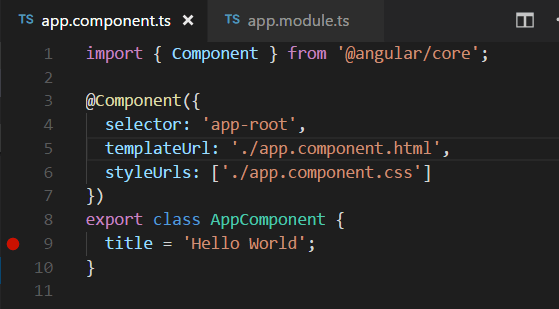
\includegraphics[width=0.75\linewidth]{imagenes/code/angular_components.png}
    \caption{Ejemplo de componentes de angular con código Typescript}
    \label{fig:angular_components}
\end{figure}

Angular es parte de un conjunto más amplio de herramientas y tecnologías de Google, por lo que su integración con otros servicios de Google es fluida. A lo largo de los años, ha ganado popularidad en el desarrollo frontend, especialmente en entornos empresariales, debido a su capacidad para manejar aplicaciones de gran escala y su enfoque en la modularidad y reutilización de código.

Uno de los lenguajes fundamentales que se utiliza en Angular es TypeScript, que proporciona características de programación orientada a objetos como clases, interfaces y herencia, facilitando el desarrollo de aplicaciones más mantenibles. Este lenguaje lo hace ideal para proyectos de gran tamaño, donde el control de tipos puede ayudar a reducir errores. A pesar de ser un framework basado en el frontend, Angular puede integrarse con varios backends, como Node.js, Django, Spring, entre otros.

Angular es un framework respaldado por Google, lo que asegura un ciclo de vida estable y una comunidad activa que contribuye a su mejora continua. Además, dado que Angular es open source, la comunidad también juega un papel clave en su evolución, lo que garantiza que el framework continúe siendo relevante en la industria del desarrollo web.

Aunque Angular es muy popular, su curva de aprendizaje puede ser algo pronunciada, especialmente para desarrolladores novatos. Además, debido a su carácter completo, puede ser excesivo para aplicaciones más pequeñas, donde un framework más ligero podría ser suficiente. Sin embargo, en proyectos de gran escala que requieren una estructura bien organizada y mantenible, Angular sigue siendo una opción sólida.

\subsection{React}
React es una biblioteca de JavaScript para la construcción de interfaces de usuario, desarrollada por Facebook (ahora Meta) \parencite{facebook}
y lanzada al público en 2013. Su principal propósito es facilitar el desarrollo de aplicaciones web interactivas y reactivas mediante un enfoque basado en componentes reutilizables. 

React se enfoca en la parte de la vista (View) en el patrón de diseño MVC (Modelo-Vista-Controlador) \parencite{MVC}, lo que permite crear interfaces dinámicas sin tener que recargar la página web.

Una de las características más destacadas de React es su uso del DOM virtual (Virtual DOM) \parencite{virtual-dom}, que mejora significativamente el rendimiento al minimizar la manipulación directa del DOM del navegador. En lugar de modificar el DOM completo con cada cambio, React crea una copia del DOM en memoria y solo actualiza las partes que han cambiado, lo que hace que las aplicaciones sean más rápidas y eficientes.

\begin{figure}
    \centering
    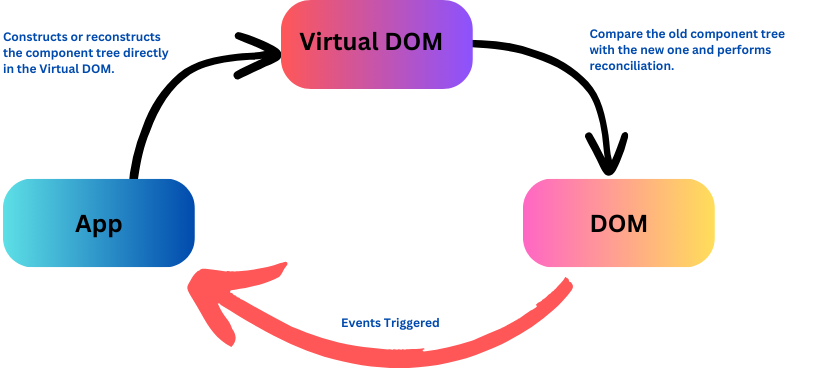
\includegraphics[width=0.75\linewidth]{imagenes/scheme/react_virtual_dom.png}
    \caption{Ejemplo de DOM virtual de React hecho por Angular Minds}
    \label{fig:react_virtual_dom}
\end{figure}

React está escrito en JavaScript, pero con soporte extendido para JSX (JavaScript XML) \parencite{JSX}
, una extensión de sintaxis que permite escribir elementos de la interfaz de usuario de forma declarativa, como si fueran parte del código HTML. Esto facilita a los desarrolladores visualizar claramente la estructura del componente dentro del código JavaScript, simplificando el desarrollo y mantenimiento de la interfaz.

El ecosistema de React ha crecido enormemente desde su lanzamiento. Aunque originalmente fue concebido para aplicaciones de una sola página (SPA), React ha evolucionado para ser usado tanto en el desarrollo frontend como en aplicaciones móviles, mediante el uso de React Native. Esto convierte a React en una tecnología versátil, usada en una amplia variedad de plataformas.

Una ventaja importante de React es su flexibilidad: no impone una arquitectura rígida y se puede integrar fácilmente con otras bibliotecas o frameworks. 

A pesar de sus ventajas, React tiene algunas desventajas. Una de ellas es que, aunque es fácil de aprender para pequeños proyectos, gestionar el estado en aplicaciones grandes puede volverse complicado, lo que requiere el uso de bibliotecas externas como Redux o Context API. Además, React es solo una biblioteca para la vista, lo que significa que carece de muchas funcionalidades de un framework completo, como el enrutamiento o la gestión de dependencias, que deben añadirse manualmente.

React ha ganado una enorme popularidad desde su lanzamiento y sigue siendo una de las bibliotecas más utilizadas para el desarrollo web, debido a su eficiencia, flexibilidad y soporte por parte de una comunidad muy activa.

\subsection{ Spring }
Spring es un marco de trabajo (framework) para el desarrollo de aplicaciones en Java, como sostiene \cite{spring-def}
, ampliamente utilizado en entornos empresariales debido a su flexibilidad y capacidad para facilitar el desarrollo de aplicaciones robustas y escalables. Fue desarrollado por Rod Johnson y lanzado inicialmente en 2003, como una alternativa ligera a los frameworks Java más pesados de la época. Spring permite construir aplicaciones que siguen los principios de inyección de dependencias y programación orientada a aspectos \cite{aop}
, lo que mejora la modularidad y facilita la gestión de la complejidad en proyectos grandes.



El propósito principal de Spring es simplificar el desarrollo de aplicaciones en Java, proporcionando una infraestructura sólida que resuelve los problemas comunes en la creación de aplicaciones de servidor. Además de su flexibilidad, Spring se destaca por sus capacidades de integración con otros frameworks y tecnologías, lo que lo convierte en una solución versátil para la creación de aplicaciones web, \gls{api}
y microservicios.

Spring es el framework base que se extiende a través de módulos como Spring MVC (para aplicaciones web), Spring Security (para control de acceso) y Spring Data (para gestión de bases de datos). Gracias a su popularidad, sigue siendo el framework Java más utilizado para el desarrollo de aplicaciones empresariales a nivel global.

\subsection{ Spring Boot }
Spring Boot es una extensión del framework Spring que fue publicada en 2014 por Pivotal Software. Está diseñada para simplificar el proceso de configuración y arranque de las aplicaciones desarrolladas en Spring. Mientras que Spring ofrece una gran flexibilidad, su configuración puede ser tediosa y propensa a errores. Aquí es donde Spring Boot aporta su valor: reduce la necesidad de configuración manual gracias a las convenciones predeterminadas y a una serie de herramientas integradas como JPA (que explicaremos más adelante), Spring Web \parencite{spring-security} y muchas más.

Spring Boot permite a los desarrolladores centrarse en la lógica del negocio en lugar de en la configuración del entorno, ya que automatiza la mayor parte de la configuración, incluyendo el servidor web, la integración con bases de datos y la seguridad. Esto es posible gracias a la división en las capas: vista (view) o cliente (client), controlador (controller), servicio (service), modelo (model) y repositorio (repository) entre otras, como se ve en la figura \ref{fig:spring_boot_layers}.   


\begin{figure}
        \centering
        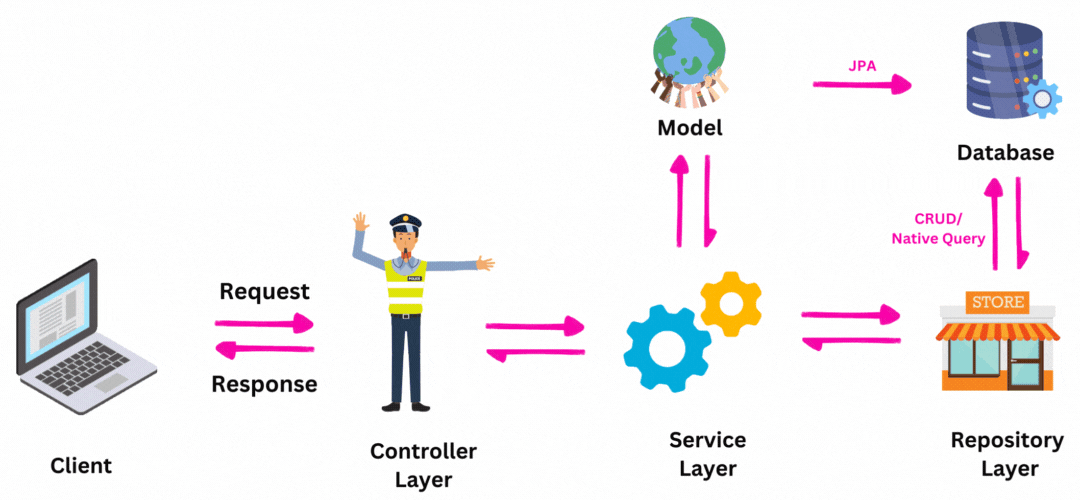
\includegraphics[width=0.75\linewidth]{imagenes/scheme/spring_boot_layers.png}
        \caption{Capas de Spring Boot hecho por Medium}
        \label{fig:spring_boot_layers}
    \end{figure}
    
    \todo{añande fuente al caption de las figuras poniendo autor o fuente parentside? la forma de citar con el nombre del autor y la fecha (perez, 2008)}

Esto lo convierte en una excelente opción para la creación rápida de prototipos, aplicaciones de producción listas para el despliegue y microservicios. Su popularidad ha crecido rápidamente debido a la eficiencia que proporciona, lo que ha hecho que muchos desarrolladores lo elijan para proyectos grandes y pequeños.

Spring Boot se integra fácilmente con otros componentes de Spring, como Spring Security y Spring Data, y se basa en las mismas buenas prácticas que han hecho de Spring un estándar en la industria del desarrollo de software. Por ejemplo, Spring Boot facilita la integración con JPA, el cual permite la persistencia de datos en bases de datos relacionales.

\subsection{ JPA }

JPA (Java Persistence API) es una especificación que simplifica la interacción con bases de datos en aplicaciones Java. Fue introducida en 2006 como parte de la plataforma Java EE 5 y desarrollada por Oracle. Su objetivo es facilitar el mapeo de objetos Java a tablas de bases de datos relacionales sin la necesidad de escribir SQL manualmente. Con JPA, los desarrolladores pueden centrarse en el código de negocio sin preocuparse por los detalles de la persistencia.

Una de las grandes ventajas de JPA es que reduce la cantidad de código repetitivo necesario para realizar operaciones CRUD (Crear, Leer, Actualizar y Borrar) en la base de datos. 

JPA permite que los desarrolladores trabajen con objetos de dominio directamente, delegando la gestión de las transacciones y el acceso a la base de datos en el framework subyacente. En combinación con Spring Data JPA, la interacción con la base de datos se hace más sencilla y eficiente, eliminando la necesidad de escribir consultas SQL explícitas en la mayoría de los casos.

JPA se utiliza principalmente en aplicaciones que requieren una gestión compleja de datos, y su integración con Spring Boot a través de Spring Data JPA permite acelerar el desarrollo al proporcionar un enfoque estandarizado para la persistencia de datos.



\subsection{ Maven }

Maven es una herramienta de gestión de proyectos y de automatización de construcción para aplicaciones Java, desarrollada por Apache Software Foundation y lanzada en 2004. 

Su principal función es gestionar las dependencias de un proyecto, es decir, todas las bibliotecas externas que el proyecto necesita para funcionar. Maven permite a los desarrolladores definir estas dependencias en un archivo XML (pom.xml) y luego descarga automáticamente las versiones correctas de estas bibliotecas desde repositorios remotos.

Una de las mayores ventajas de Maven es su capacidad para estandarizar el proceso de construcción de aplicaciones Java, independientemente del entorno en el que se desarrolle. Esto asegura que los proyectos construidos con Maven sean consistentes y que se puedan replicar fácilmente en cualquier máquina de desarrollo.

En este proyecto, Maven juega un papel crucial al manejar las dependencias de Spring Boot, JPA y Thymeleaf, asegurando que todas las bibliotecas necesarias estén disponibles y configuradas correctamente.

\subsection{ Thymeleaf }

Thymeleaf es un motor de plantillas para aplicaciones Java, creado por Daniel Fernández en 2011, que permite la generación dinámica de contenido HTML, XML y otros formatos de texto. 

Thymeleaf se usa principalmente para construir la vista (view) o plantilla (template) en aplicaciones web, y es altamente compatible con Spring, ya que facilita la integración de los modelos de datos Java con las plantillas HTML de manera eficiente.

Una de las principales ventajas de Thymeleaf es que permite crear plantillas que pueden ser previsualizadas sin necesidad de ejecutar la aplicación en un servidor. Esto lo hace particularmente útil para el desarrollo colaborativo entre diseñadores y programadores, ya que los archivos HTML son completamente editables desde el lado del cliente.

Thymeleaf está diseñado para funcionar bien con Spring MVC y Spring Boot, lo que lo convierte en una opción natural para las aplicaciones web que necesitan generar contenido dinámico basado en datos proporcionados por el servidor.


    



    
    \section{Ciberseguridad}
\label{sec:ciberseguridad}

La ciberseguridad es un aspecto crítico en el desarrollo de aplicaciones modernas, especialmente cuando se manejan datos sensibles como credenciales de usuarios, información personal, contraseñas y documentos privados. En este apartado, se describen las tecnologías y prácticas más relevantes en el ámbito de la ciberseguridad, con un enfoque en el cifrado de datos y las capas de seguridad en el proceso de autenticación.

\subsection{Cifrado}
\label{subsec:cifrado}

El cifrado es una técnica fundamental para proteger la confidencialidad e integridad de los datos. Consiste en transformar la información en un formato ilegible para cualquier persona que no posea la clave de descifrado adecuada. A continuación, se describen los principales enfoques y tecnologías utilizadas en el cifrado de datos.

\subsubsection{Cifrado Simétrico}

El cifrado simétrico utiliza una única clave para cifrar y descifrar los datos. Este enfoque es eficiente en términos de rendimiento, ya que requiere menos recursos computacionales en comparación con el cifrado asimétrico. Sin embargo, la gestión segura de la clave es un desafío, ya que debe compartirse entre las partes que necesitan cifrar y descifrar los datos.

\begin{itemize}
    \item \textbf{AES (Advanced Encryption Standard)}: Es uno de los algoritmos de cifrado simétrico más utilizados y seguros. AES opera en bloques de 128 bits y admite claves de 128, 192 o 256 bits. Su fortaleza radica en su resistencia a ataques criptográficos y su eficiencia en términos de velocidad.
    \item \textbf{Modos de operación}: AES puede utilizarse en diferentes modos de operación, como ECB (Electronic Codebook), CBC (Cipher Block Chaining) y GCM (Galois/Counter Mode). Cada modo tiene sus propias características y niveles de seguridad.
\end{itemize}

\subsubsection{Cifrado Asimétrico}

El cifrado asimétrico, también conocido como cifrado de clave pública, utiliza un par de claves: una clave pública para cifrar los datos y una clave privada para descifrarlos. Este enfoque es ideal para escenarios donde la clave no puede compartirse de manera segura, como en la comunicación entre dos partes que no han establecido previamente una relación de confianza.

\begin{itemize}
    \item \textbf{RSA (Rivest-Shamir-Adleman)}: Es uno de los algoritmos de cifrado asimétrico más populares. RSA se basa en la dificultad de factorizar números grandes en sus componentes primos. Aunque es seguro, su rendimiento es inferior al cifrado simétrico, por lo que se utiliza principalmente para cifrar claves o datos pequeños.
    \item \textbf{Curvas Elípticas (ECC)}: Es una alternativa más moderna y eficiente a RSA. ECC ofrece un nivel de seguridad similar con claves más cortas, lo que reduce el consumo de recursos y mejora el rendimiento.
\end{itemize}

\subsubsection{Cifrado de Contraseñas}

El cifrado de contraseñas es un caso especial donde se utilizan funciones de hash unidireccionales para almacenar las contraseñas de manera segura. A diferencia del cifrado tradicional, el hash no puede revertirse, lo que garantiza que incluso si la base de datos es comprometida, las contraseñas no puedan recuperarse.

\begin{itemize}
    \item \textbf{BCrypt}: Es una función de hash diseñada específicamente para contraseñas. BCrypt utiliza un valor de "salt" único para cada contraseña, lo que aumenta la seguridad frente a ataques de diccionario y fuerza bruta. Además, su diseño permite ajustar la complejidad del hashing, lo que lo hace resistente a los avances en hardware.
    \item \textbf{Argon2}: Es una función de hash moderna que ha ganado popularidad debido a su resistencia a ataques de fuerza bruta y su capacidad para utilizar múltiples recursos del sistema (CPU, memoria y paralelismo). Argon2 es considerado uno de los algoritmos más seguros para el cifrado de contraseñas.
\end{itemize}

\subsection{Capas de Seguridad en el Login}
\label{subsec:capas-seguridad-login}

El proceso de autenticación es uno de los puntos más vulnerables en cualquier aplicación, ya que es el primer paso para acceder a los recursos protegidos. Para garantizar la seguridad del login, es esencial implementar múltiples capas de seguridad que protejan contra ataques comunes y refuercen la integridad del sistema.

\subsubsection{Protección contra Ataques de Fuerza Bruta}

Los ataques de fuerza bruta intentan adivinar las credenciales de un usuario probando múltiples combinaciones de nombres de usuario y contraseñas. Para proteger contra estos ataques, es esencial implementar medidas como:

\begin{itemize}
    \item \textbf{Límite de Intentos}: Bloquear temporalmente la cuenta después de un número determinado de intentos fallidos. Esto dificulta que un atacante pueda probar múltiples combinaciones en un corto período de tiempo.
    \item \textbf{CAPTCHA}: Requerir que el usuario resuelva un desafío CAPTCHA después de varios intentos fallidos. Esto ayuda a distinguir entre usuarios legítimos y bots automatizados.
\end{itemize}

\subsubsection{Protección contra Ataques CSRF (Cross-Site Request Forgery)}

Los ataques CSRF explotan la confianza que un sitio web tiene en el navegador del usuario para realizar acciones no autorizadas. Para prevenir estos ataques, se pueden implementar las siguientes medidas:

\begin{itemize}
    \item \textbf{Tokens CSRF}: Generar un token único para cada sesión de usuario y validarlo en cada solicitud. Esto garantiza que la solicitud proviene de una fuente legítima.
    \item \textbf{SameSite Cookies}: Configurar las cookies con el atributo \textbf{SameSite} para evitar que se envíen en solicitudes cruzadas entre sitios.
\end{itemize}

\subsubsection{Registro y Monitoreo de Actividad}

El registro y monitoreo de la actividad del usuario es esencial para detectar y responder a posibles amenazas de seguridad. Algunas prácticas recomendadas incluyen:

\begin{itemize}
    \item \textbf{Registro de Accesos}: Registrar todos los intentos de login, tanto exitosos como fallidos, para identificar patrones sospechosos.
    \item \textbf{Alertas de Seguridad}: Configurar alertas para notificar a los administradores en caso de actividades inusuales, como múltiples intentos fallidos de login desde diferentes ubicaciones.
\end{itemize}


\section{Diseño software}
El diseño de software es una fase crítica en el desarrollo de aplicaciones, ya que define la estructura, organización y comportamiento del sistema. Un buen diseño no solo garantiza que el software cumpla con los requisitos funcionales, sino que también facilita su mantenimiento, escalabilidad y reutilización. En este apartado, se abordarán los patrones de diseño más comunes y los diagramas UML, herramientas esenciales para modelar y documentar sistemas de software.

\subsection{Patrones de diseño software}
\todo{buscar estudio} Los patrones de diseño son soluciones probadas y reutilizables para problemas comunes en el desarrollo de software. Estos patrones proporcionan un enfoque estructurado para resolver desafíos específicos, mejorando la calidad del código y facilitando su mantenimiento. A continuación, se describen algunos de los patrones más utilizados:

\subsubsection{Patrón Fachada (Facade)}
El patrón Fachada es un patrón estructural que proporciona una interfaz simplificada para un conjunto de interfaces en un subsistema. Este patrón es útil cuando un sistema es complejo y tiene múltiples componentes, ya que oculta la complejidad detrás de una interfaz única y fácil de usar. Por ejemplo, en una aplicación con múltiples servicios y bibliotecas, una fachada puede actuar como un punto de entrada único, reduciendo la dependencia entre los componentes y facilitando su uso.

\subsubsection{Patrón Singleton}
El patrón Singleton es un patrón creacional que garantiza que una clase tenga una única instancia y proporciona un punto de acceso global a esa instancia. Este patrón es útil cuando se necesita un único punto de control, como en la gestión de configuraciones, conexiones a bases de datos o registros de logs. Al garantizar que solo exista una instancia, se evita la duplicación de recursos y se asegura un comportamiento consistente en toda la aplicación.

\subsubsection{Otros patrones comunes}
Además de los mencionados, existen otros patrones ampliamente utilizados, como:
\begin{itemize}
    \item \textbf{Patrón Observador (Observer)}: Permite que un objeto notifique a otros objetos sobre cambios en su estado.
    \item \textbf{Patrón Estrategia (Strategy)}: Define una familia de algoritmos, encapsula cada uno de ellos y los hace intercambiables.
    \item \textbf{Patrón Inyección de Dependencias (Dependency Injection)}: Facilita la gestión de dependencias entre componentes, promoviendo un código más modular y testeable.
\end{itemize}

\subsection{Diagramas UML}
\todo{buscar estudio} El Lenguaje Unificado de Modelado (UML, por sus siglas en inglés) es un estándar utilizado para visualizar, especificar, construir y documentar sistemas de software. Los diagramas UML son una herramienta esencial para comunicar el diseño del software entre desarrolladores, analistas y stakeholders. A continuación, se describen los tipos de diagramas más relevantes.

\subsubsection{Diagrama de secuencia UML}
El diagrama de secuencia es un tipo de diagrama de interacción que muestra cómo los objetos interactúan en un escenario específico a lo largo del tiempo. Este diagrama es especialmente útil para modelar el flujo de mensajes entre objetos en un sistema, lo que permite entender cómo se ejecutan las operaciones y en qué orden.

\begin{itemize}
    \item \textbf{Actores}: Representan los roles externos que interactúan con el sistema, como usuarios o sistemas externos.
    \item \textbf{Objetos}: Representan las instancias de clases o componentes del sistema.
    \item \textbf{Mensajes}: Representan las interacciones entre objetos, mostrando el flujo de control y datos.
    \item \textbf{Línea de vida}: Muestra la existencia de un objeto durante el tiempo de ejecución.
\end{itemize}

Los diagramas de secuencia son ideales para modelar casos de uso complejos, como procesos de autenticación, transacciones o flujos de trabajo. Además, son una herramienta valiosa para identificar cuellos de botella y optimizar el rendimiento del sistema.

\subsubsection{Otros diagramas UML}
Además del diagrama de secuencia, UML incluye otros tipos de diagramas, como:
\begin{itemize}
    \item \textbf{Diagrama de clases}: Muestra la estructura estática del sistema, incluyendo clases, atributos, métodos y relaciones.
    \item \textbf{Diagrama de casos de uso}: Representa las interacciones entre los actores y el sistema, describiendo las funcionalidades desde la perspectiva del usuario.
    \item \textbf{Diagrama de actividades}: Modela el flujo de trabajo o procesos de negocio, mostrando las actividades y decisiones involucradas.
    \item \textbf{Diagrama de componentes}: Muestra la organización física del sistema, incluyendo módulos, bibliotecas y dependencias.
\end{itemize}

En resumen, los patrones de diseño y los diagramas UML son herramientas fundamentales en el desarrollo de software moderno. Los patrones de diseño proporcionan soluciones reutilizables para problemas comunes, mientras que los diagramas UML facilitan la comunicación y documentación del diseño del sistema. Juntos, permiten crear aplicaciones robustas, mantenibles y escalables.

    
\chapter{Metodología} \label{metodologia}

\section{ Gestión del trabajo }

A lo largo de mi etapa universitaria, he procurado aplicar de manera rigurosa las diversas metodologías y enfoques de desarrollo adquiridos en clase, con el fin de abordar de manera eficiente y estructurada los proyectos en los que he participado. Cada proyecto ha sido una oportunidad para poner en práctica los conocimientos teóricos y refinar mis habilidades técnicas, adaptándome a las demandas específicas de cada entorno.

En particular, he implementado un sistema de trabajo basado en revisiones periódicas y planificación semanal. Estas revisiones, que se llevaban a cabo con el tutor de la empresa colaboradora, incluían el análisis de los diagramas de secuencia UML correspondientes a las tareas previstas para la semana y la evaluación del trabajo realizado en la semana anterior, a través de una sesión de code review. Esta dinámica no solo permitía detectar y corregir posibles errores, sino que también abría espacio para sugerir mejoras en la arquitectura y el código, asegurando que el desarrollo se mantuviera alineado con los objetivos del proyecto.

Además, la rutina diaria de reuniones con el tutor permitía una constante actualización y reajuste de las prioridades y tareas a realizar. Estas reuniones breves pero efectivas garantizaban que el equipo estuviera siempre sincronizado y que cualquier cambio en los requisitos o en la planificación fuera rápidamente incorporado, optimizando así el flujo de trabajo y manteniendo una comunicación fluida entre todos los involucrados. Este enfoque ágil ha sido clave para llevar a cabo desarrollos de calidad y adaptables a posibles contingencias del proyecto.

\section{ Metodología de proyecto }

De las opciones de las posibles tecnologías para llevar a cabo del proyecto abordadas en el estado de la cuestión, estas son las que se han elegido:

\subsection{ Spring boot }
Aunque existen otros frameworks populares hoy en día, como Angular y React, estos están basados en JavaScript, un lenguaje diferente de Java. JavaScript es más versátil al permitir el desarrollo tanto en frontend como en backend, pero presenta desventajas en términos de seguridad. Al no ser un lenguaje tipado ni ejecutarse en una máquina virtual, es más vulnerable a ciertos tipos de ataques, como se explica en este artículo \cite{java-vs-javascript}. Por esta razón, para este proyecto fue necesario optar por un framework que utilizara Java.

Spring Boot ha sido la tecnología seleccionada para el desarrollo de esta aplicación web debido a sus características que facilitan la creación de aplicaciones empresariales robustas y escalables. 

Dado que el proyecto se centra en la monitorización de documentos en un entorno bancario, donde la seguridad, eficiencia y fiabilidad son aspectos clave, Spring Boot proporciona una base sólida. Con su configuración mínima y capacidades integradas, permite un desarrollo rápido y efectivo, adaptándose a las necesidades de este entorno.

Una de las principales ventajas de Spring Boot es su capacidad para simplificar el desarrollo de aplicaciones complejas gracias a su amplia gama de bibliotecas y configuraciones predeterminadas. Su integración con tecnologías como Spring Security facilita la implementación de controles de acceso y autenticación, esenciales en un entorno bancario. Además, su soporte para la gestión eficiente de bases de datos mediante JPA es ideal para manejar grandes volúmenes de datos, como los documentos almacenados en esta aplicación.

Otra ventaja importante para el uso de Spring Boot es la popularidad de Java, ya que es el séptimo lenguaje de programación más usado por profesionales según stack overflow como se puede ver en la figura 5.1 \footnote{ Most used tech \href{https://survey.stackoverflow.co/2024/technology\#most-popular-technologies-language}{Stack Overflow}}. Cabe destacar en popularidad también al propio framework Spring Boot, que es el undécimo framework de desarrollo más utilizado en el mundo, como se muestra en la figura 5.2. Esto garantiza que la tecnología continúe evolucionando, lo que asegura la viabilidad del proyecto a largo plazo, además de la abundante documentación y comunidad de soporte. Spring Boot también es uno de los frameworks preferidos por los bancos, como se destaca en estudios especializados\footnote{Why banks, Visa, and Mastercard prefer Java and Spring Boot for their backend \href{https://medium.com/@YodgorbekKomilo/why-banks-visa-and-mastercard-prefer-java-and-spring-boot-for-their-backend-and-server-3db88940f594}{Medium}}. Esto se debe a su robustez, estabilidad, seguridad y escalabilidad, características clave en aplicaciones empresariales críticas.

\begin{figure}
    \centering
    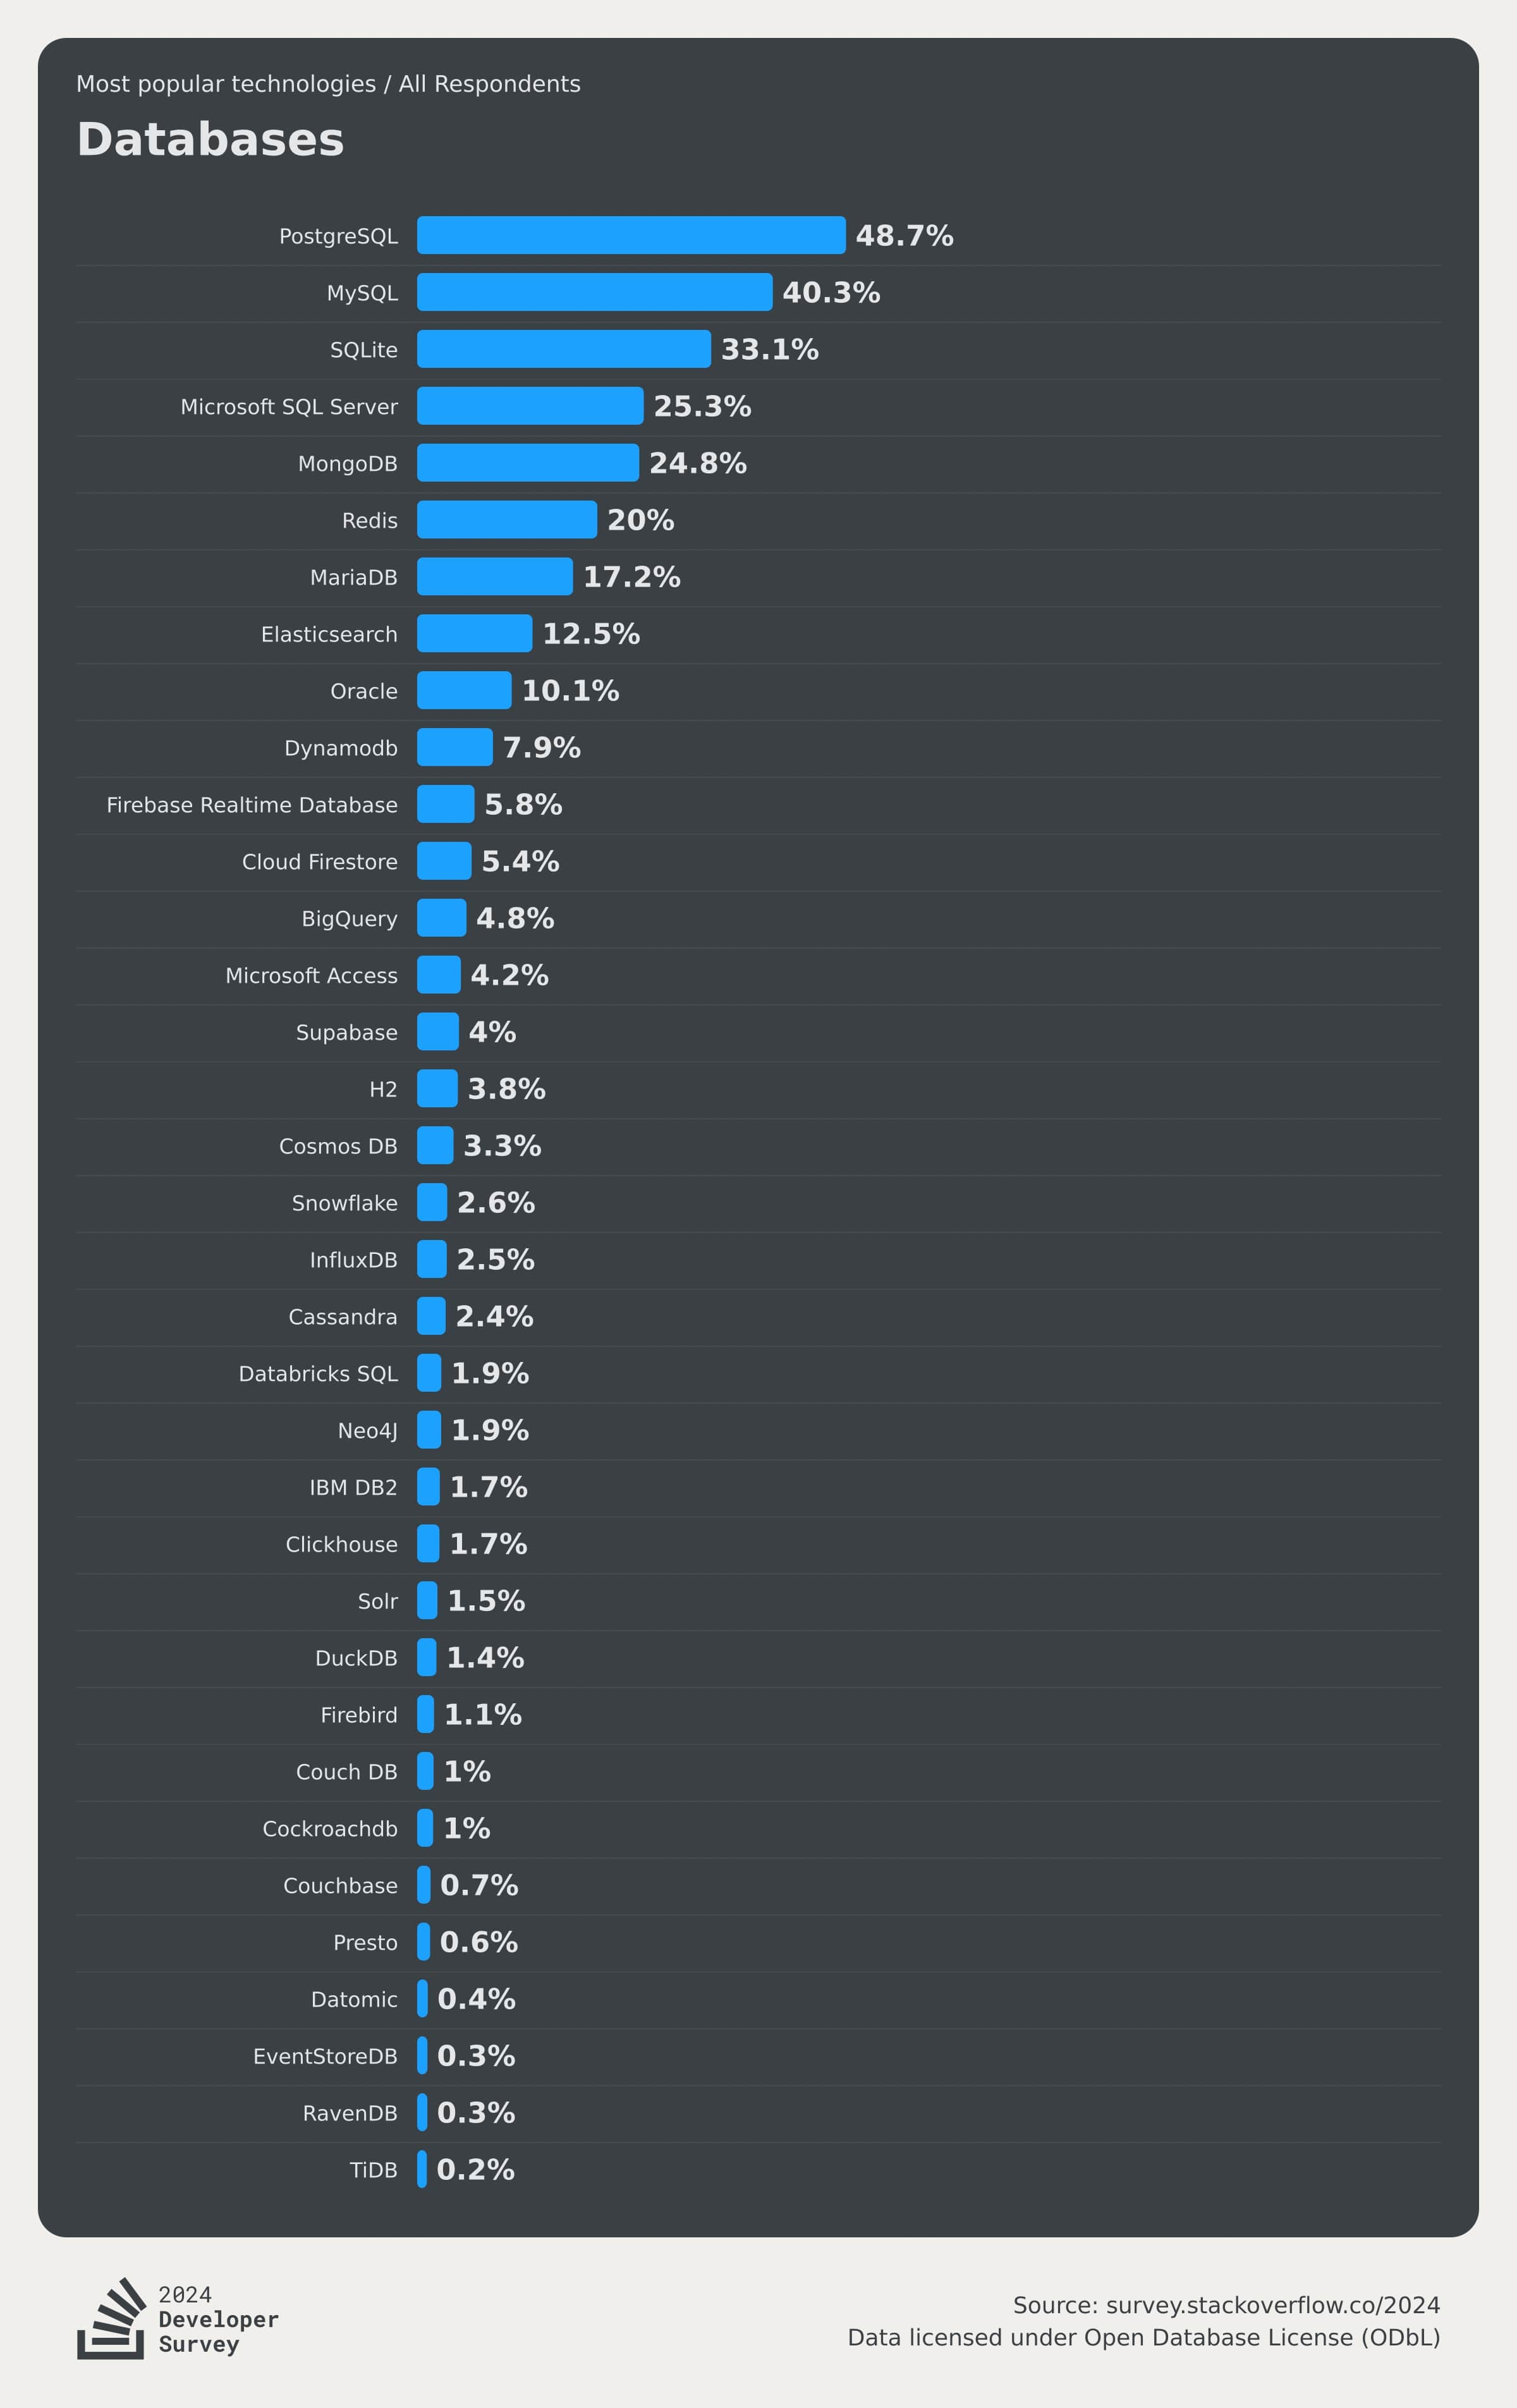
\includegraphics[width=0.85\linewidth]{imagenes/charts/java_stadistics.jpg}
    \caption{Tecnologías más populares hecho por StackOverflow}
    \label{fig:most-used-tech}
\end{figure}

\begin{figure}
    \centering
    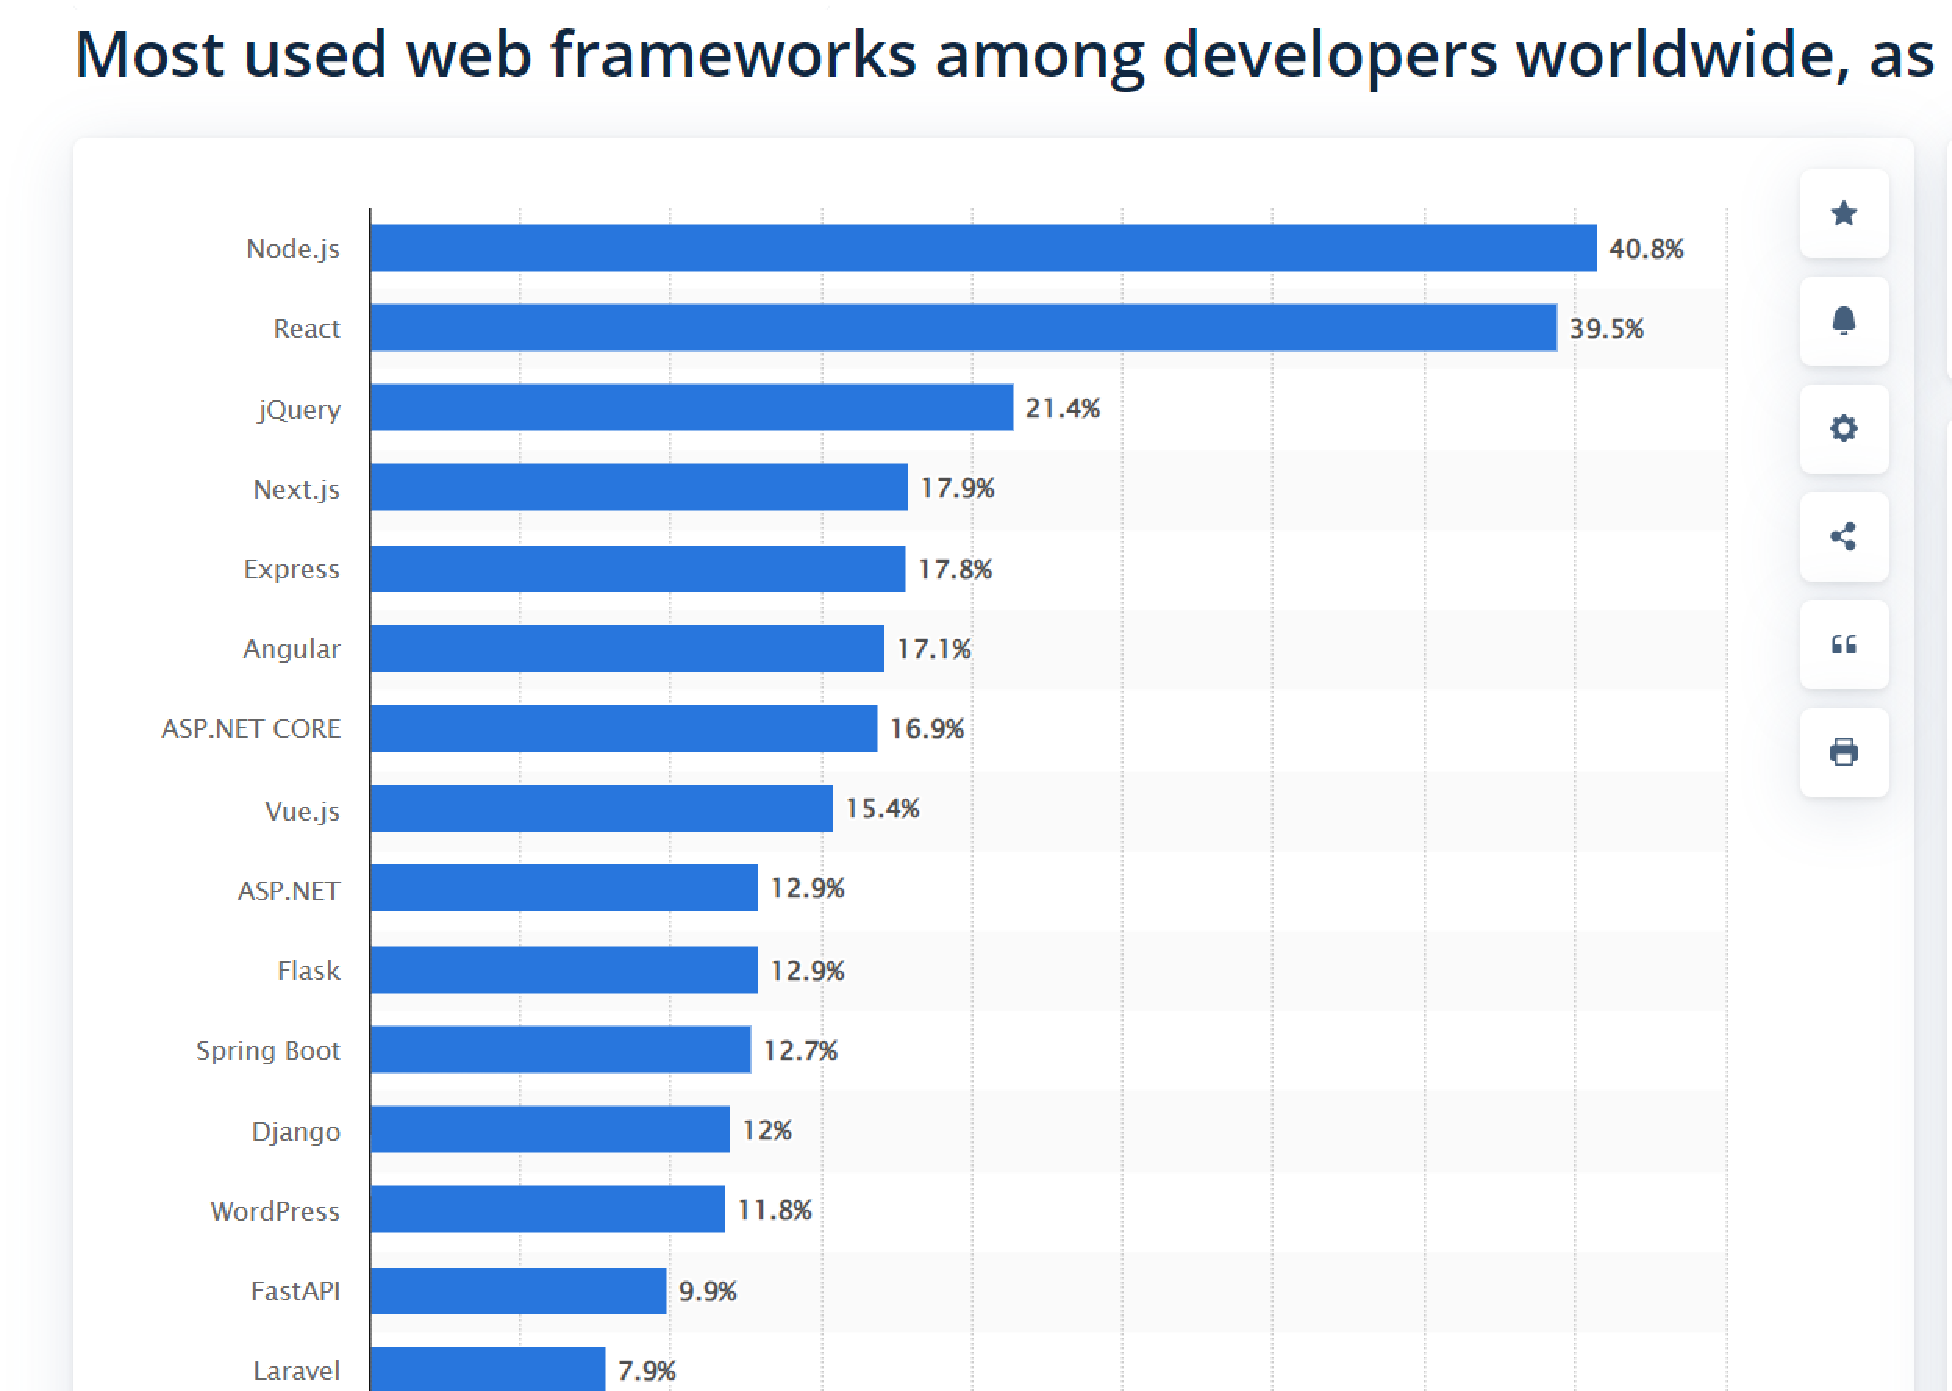
\includegraphics[width=0.9\linewidth]{imagenes/charts/spring_boot_stadistics.pdf}
    \caption{Frameworks web más usados por desarrolladores en el mundo hecho por Stalista}
    \label{fig:most-used-frameworks}
\end{figure}



No obstante, el uso de Spring Boot también presenta ciertos inconvenientes. Aunque su automatización y configuraciones predeterminadas aceleran el desarrollo, en proyectos a gran escala pueden generar una sobrecarga de recursos si no se optimizan adecuadamente. La facilidad para incluir dependencias adicionales puede aumentar la complejidad del proyecto, afectando al rendimiento y a la mantenibilidad del código a largo plazo.

Otro aspecto a considerar es que, al estar basado en Java, Spring Boot puede requerir mayores recursos de memoria y procesamiento en comparación con tecnologías más ligeras. Esto puede ser un reto en servidores con limitaciones de hardware o cuando se buscan optimizaciones de recursos.

A pesar de estos inconvenientes, Spring Boot sigue siendo una opción sólida y flexible para desarrollar aplicaciones empresariales seguras y escalables, como es el caso de esta solución para la gestión documental en entornos bancarios.

\subsection{ Maven }

Maven ha sido elegido como la herramienta de gestión de dependencias y automatización de la construcción para este proyecto debido a su fiabilidad y popularidad en el ecosistema Java. Una de las principales razones por las que Maven es ampliamente utilizado en proyectos empresariales es su capacidad para simplificar la gestión de dependencias, lo que facilita la integración de bibliotecas externas necesarias para el correcto funcionamiento de la aplicación.

Una ventaja significativa de Maven es su capacidad para gestionar de manera eficiente las versiones de las dependencias y sus transitorios, asegurando que siempre se utilicen versiones compatibles y actualizadas de las bibliotecas, lo que es crucial para mantener la seguridad y estabilidad del proyecto en el tiempo. Además, Maven proporciona una estructura de proyecto estándar y bien organizada, lo que facilita la colaboración entre distintos equipos y la integración con herramientas de CI/CD (Integración Continua y Entrega Continua).

Según la encuesta de Stack Overflow, Maven es una de las herramientas de automatización de construcción más usadas en el mundo, lo que garantiza una amplia documentación y soporte por parte de la comunidad \footnote{Most popular tech \href{https://survey.stackoverflow.co/2024/technology\#most-popular-technologies-tools}{Stack Overflow}}. Esto asegura la viabilidad de su uso a largo plazo, además de la fácil capacitación de nuevos desarrolladores que se unan al proyecto.

Sin embargo, uno de los inconvenientes de Maven es su curva de aprendizaje inicial, especialmente para desarrolladores que no están familiarizados con su configuración basada en XML. Además, en proyectos de gran escala, la acumulación de dependencias puede generar archivos de configuración extensos y difíciles de manejar si no se estructuran adecuadamente. Otro aspecto a considerar es el tiempo de compilación, que puede ser considerable en proyectos grandes debido a la resolución de dependencias y la construcción de los módulos.

A pesar de estos inconvenientes, Maven sigue siendo la opción ideal para este proyecto, ya que proporciona una solución integral para la gestión de dependencias y la automatización de la construcción, permitiendo un desarrollo ágil y organizado.

\subsection{ Thymeleaf }

Thymeleaf ha sido seleccionado como el motor de plantillas para el desarrollo del frontend de esta aplicación debido a su estrecha integración con Spring Boot y su capacidad para crear vistas dinámicas basadas en HTML. Al ser una tecnología diseñada específicamente para aplicaciones web Java, Thymeleaf permite renderizar páginas de manera eficiente, con una sintaxis que resulta intuitiva para los desarrolladores que ya están familiarizados con HTML y CSS.

Una de las principales ventajas de Thymeleaf es que permite construir plantillas que son directamente visualizables en navegadores, incluso sin un servidor backend activo, lo que agiliza el desarrollo de interfaces. Esto se alinea con la necesidad de este proyecto de desarrollar una aplicación web accesible y fácil de mantener. Además, Thymeleaf soporta la validación de formularios y la internacionalización, características clave para una aplicación que pueda ser utilizada en distintos contextos empresariales y por usuarios de diversas regiones.

Según la propia web de Thymeleaf, es uno de los motores de plantillas más populares dentro del ecosistema de Spring, ya que tiene más de un millón y medio de descargas al mes, lo que asegura la existencia de abundante documentación y ejemplos prácticos \footnote{Who is using thymeleaf? \href{https://www.thymeleaf.org/whoisusingthymeleaf.html}{Thymeleaf}}. Esto facilita su integración y reduce la curva de aprendizaje para nuevos desarrolladores.

\begin{figure}
    \centering
    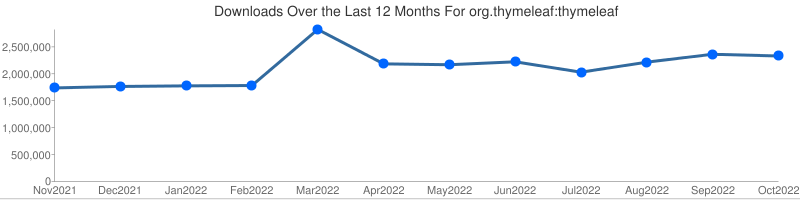
\includegraphics[width=0.75\linewidth]{imagenes/charts/thymeleaf_usage.png}
    \caption{Descargas mensuales de Thymeleaf, autor Thymeleaf}
    \label{fig:descargas_mensuales_thymeleaf}
\end{figure}

No obstante, Thymeleaf presenta algunos inconvenientes. Al ser un motor de plantillas del lado del servidor, puede tener un rendimiento inferior en comparación con soluciones de frontend basadas en JavaScript, como React o Angular, especialmente cuando se trata de aplicaciones con una gran cantidad de interacciones en tiempo real. Además, la generación de vistas en el servidor puede aumentar la carga de procesamiento en aplicaciones con un gran número de usuarios concurrentes, lo que puede requerir optimizaciones adicionales en el backend.

A pesar de estos desafíos, Thymeleaf sigue siendo una opción adecuada para este proyecto, ya que facilita la creación de una interfaz de usuario dinámica y bien integrada con Spring Boot, manteniendo un enfoque en la simplicidad y la seguridad, lo cual es crucial para aplicaciones bancarias y empresariales.


\subsection{ JPA }

JPA (Java Persistence API) ha sido elegido en este proyecto por su capacidad para simplificar la interacción con la base de datos, eliminando la necesidad de escribir consultas SQL manuales en la mayoría de los casos. Al trabajar con JPA, el desarrollador puede centrarse en los objetos de dominio de Java, ya que JPA se encarga de la persistencia de los datos de manera automática, permitiendo mapear las entidades directamente a las tablas de la base de datos.

Una de las principales ventajas de JPA es su capacidad para abstraer la complejidad del SQL. Esto simplifica el desarrollo al utilizar operaciones CRUD predefinidas y un lenguaje de consultas más amigable como JPQL (Java Persistence Query Language), que evita la necesidad de escribir SQL detallado. Además, JPA se integra perfectamente con Spring Data, lo que permite generar repositorios y consultas dinámicas de forma automática, lo cual mejora la productividad y reduce el riesgo de errores en la interacción con la base de datos.

\begin{figure}
    \centering
    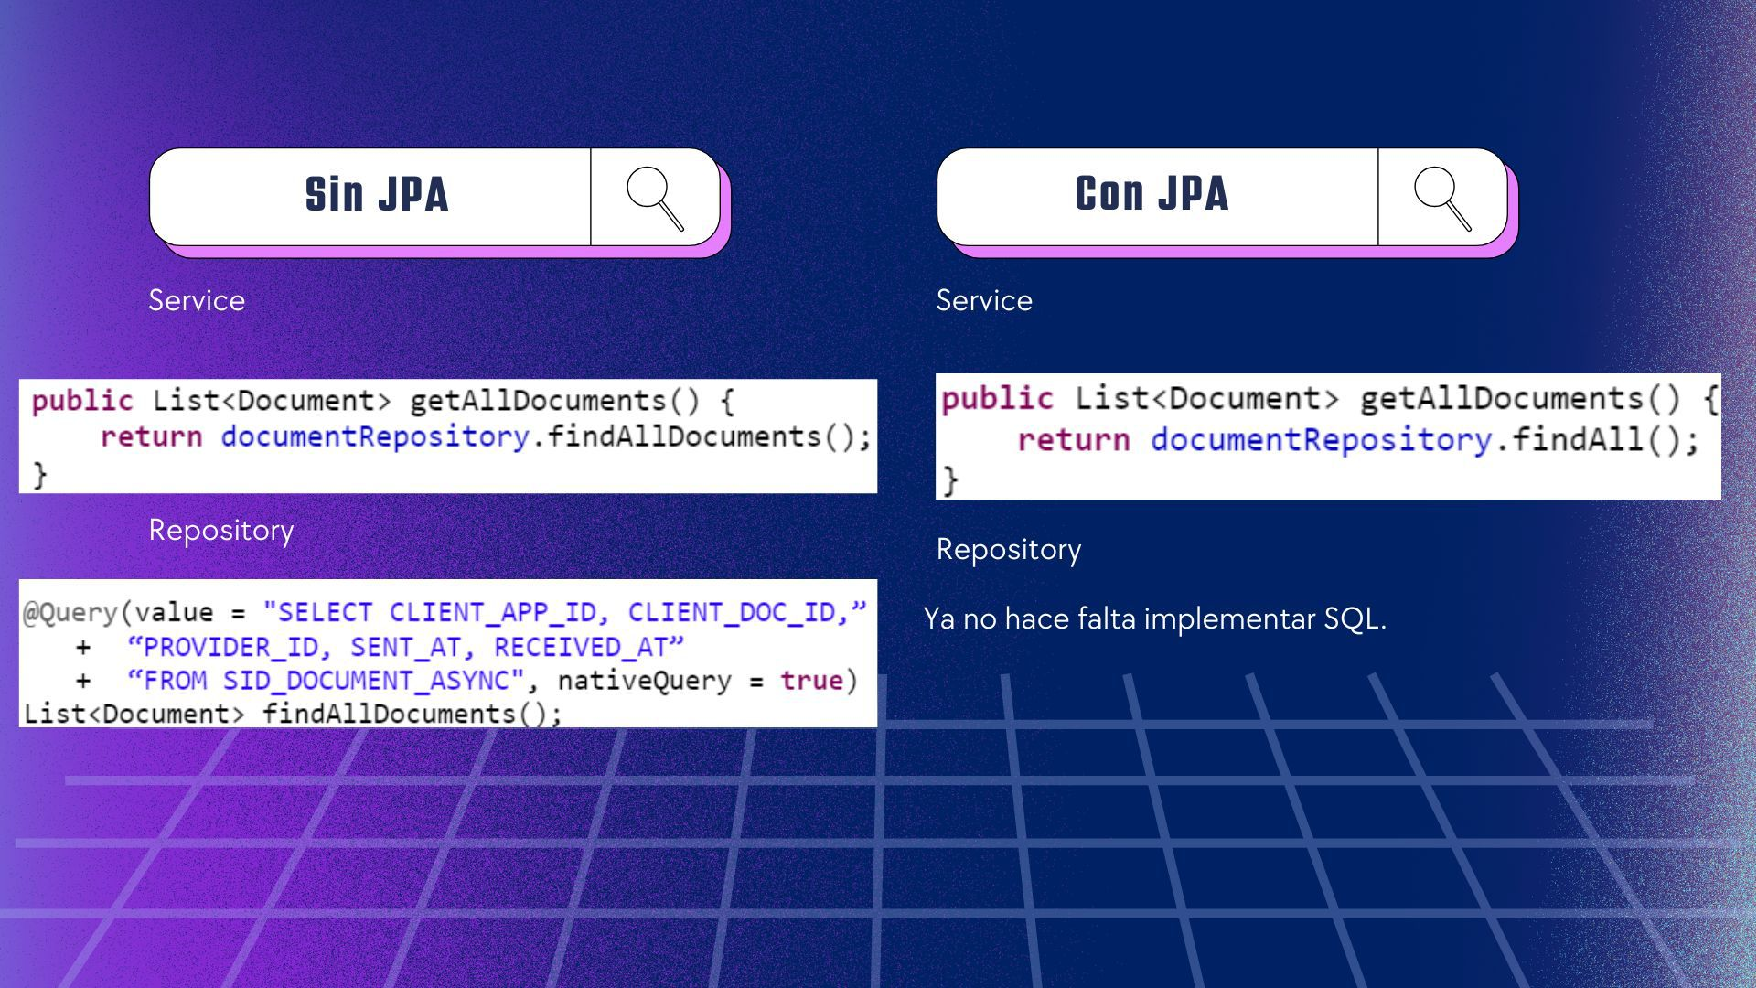
\includegraphics[width=0.75\linewidth]{imagenes/code/JPA_usage.pdf}
    \caption{Diferencia entre usar y no usar JPA, fuente propia}
    \label{fig:jpa-usage}
\end{figure}

JPA también garantiza la independencia de la base de datos, ya que facilita la migración entre distintos sistemas de gestión de bases de datos sin cambios significativos en el código. 

Sin embargo, uno de los inconvenientes de JPA es su rendimiento en escenarios con consultas SQL muy complejas o específicas, donde puede ser necesario optimizar manualmente el SQL para obtener mejores tiempos de respuesta. Además, JPA puede añadir una cierta sobrecarga en términos de recursos debido a la gestión de la caché y las transacciones automáticas.

A pesar de estos desafíos, JPA sigue siendo una opción ideal para este proyecto, ya que facilita enormemente la gestión de la persistencia de datos, minimizando la necesidad de escribir SQL manual y aumentando la eficiencia del desarrollo.



%Objetivos
\chapter{Objetivos} \label{objetivos}
El objetivo de este proyecto es desarrollar una aplicación web que permita consultar documentos almacenados en una base de datos, enfocándose en aquellos que no han sido correctamente guardados o presentan errores. Mediante el uso de filtros avanzados, los usuarios podrán identificar y gestionar de manera eficiente los metadatos de estos documentos, mejorando así la integridad y el control de la información. 
La aplicación también será escalable y segura, garantizando su adecuado funcionamiento en diversos entornos y proporcionando una herramienta útil para la gestión de bases de datos.

Los objetivos específicos son:
\begin{enumerate}
    \item \textbf{Desarrollar una interfaz web altamente usable}: El diseño de la interfaz será intuitivo y accesible, permitiendo que cualquier usuario, independientemente de su nivel de conocimientos técnicos, pueda interactuar con la aplicación sin dificultad. Esto facilitará su adopción en empresas de distintos tamaños y sectores.

    \item \textbf{Implementar un sistema basado en arquitectura cliente-servidor para ordenador}: La aplicación será accesible a través de un navegador web, sin necesidad de instalación en dispositivos locales. Funciona bajo una arquitectura cliente-servidor, donde el servidor aloja y gestiona los datos, mientras que los usuarios interactúan con la aplicación desde el cliente, facilitando así su uso en múltiples dispositivos y plataformas, sin las limitaciones de una aplicación de escritorio.
    
    \item \textbf{Implementar mecanismos de seguridad avanzados}: La aplicación incorporará diversas capas de seguridad, incluyendo autenticación de usuarios y cifrado robusto para proteger las credenciales. Se prestará especial atención a la prevención de vulnerabilidades, mediante el uso de sesiones seguras, códigos aleatorios y la gestión adecuada de estados.
    
    \item \textbf{Optimizar la eficiencia y rendimiento de la aplicación}: Se aplicarán técnicas y buenas prácticas para minimizar los tiempos de carga y garantizar que la aplicación funcione de manera rápida y eficiente, incluso cuando se maneje un gran volumen de datos.

    \item \textbf{Generar un código limpio, modular y bien documentado:} El código será diseñado para ser fácilmente reusable y mantenible, con una arquitectura desacoplada que permita modificar los inputs desde archivos externos. Además, se integrarán logs exhaustivos y documentación clara para facilitar futuras mejoras y el trabajo de otros desarrolladores.

    \item \textbf{Dominar y aplicar diagramas de secuencia UML}: Para garantizar un desarrollo estructurado y coherente, se emplearán diagramas de secuencia UML, permitiendo una planificación detallada de los flujos de trabajo y las interacciones entre los componentes del sistema.

\end{enumerate}


\chapter{Diseño} \label{disenyo}
\section{Arquitectura seleccionada}


En esta sección se describe la arquitectura seleccionada para el desarrollo del sistema, destacando la división entre el frontend y el backend, y cómo estos componentes interactúan para ofrecer una experiencia fluida al usuario. La arquitectura sigue un patrón típico de aplicaciones web basado en capas, el cual se detalla a continuación.

\subsection{Descripción de la arquitectura}

La arquitectura seleccionada se basa en el framework Spring Boot para el backend y Thymeleaf para el frontend. Este enfoque garantiza una integración robusta entre la lógica de negocio y las interfaces de usuario.

El usuario interactúa con la aplicación a través de las interfaces de frontend desarrolladas con Thymeleaf, un motor de plantillas que permite generar dinámicamente las vistas en función de los datos obtenidos desde el backend. Estas interfaces envían y reciben peticiones HTTP (HTTP requests), que son gestionadas por los controladores (controllers) en el backend.

El flujo de trabajo es el siguiente:


\begin{enumerate}
    \item View (Thymeleaf):
   El cliente accede a las interfaces visuales, las cuales están diseñadas con Thymeleaf para garantizar una generación dinámica y eficiente de las vistas. Este motor de plantillas permite incluir datos provenientes del backend directamente en las páginas HTML, facilitando la comunicación entre ambas capas.

    \item Controladores (Controller):
   Los controladores son responsables de gestionar las peticiones HTTP provenientes del frontend. Estos se encargan de procesar la solicitud y delegar la lógica de negocio al siguiente nivel, los servicios. En otras palabras, son conectores que dirigen las peticiones del usuario a los servicios correspondientes sin modificar ni hacer operaciones de lógica de negocio.

    \item Servicios (Service):
   La capa de servicios representa el núcleo de la lógica de negocio. Aquí se implementan las operaciones principales de la aplicación. Los servicios se encargan de realizar las transformaciones necesarias sobre los datos y delegan las operaciones de almacenamiento o consulta al repositorio.

    \item Repositorio (Repository):
   El repositorio representa la capa de acceso a datos. Utilizando JPA (Java Persistence API), se conecta con la base de datos para realizar operaciones CRUD (Crear, Leer, Actualizar, Eliminar). Esta capa abstrae los detalles de implementación de la base de datos, permitiendo una interacción más sencilla.

    \item Modelo de datos (Model):
   Los datos manejados por la aplicación están representados mediante entidades JPA. Estas entidades mapean las tablas de la base de datos, permitiendo que la lógica de negocio interactúe con ellas de forma directa.

    \item Base de datos:
   Finalmente, la base de datos almacena la información persistente del sistema. La conexión con esta se realiza mediante JPA, utilizando herramientas ya mencionadas en capítulos anteriores.
\end{enumerate}

\subsection{Herramientas utilizadas}

Para implementar esta arquitectura, se han empleado diversas herramientas, las cuales se mencionaron previamente. A continuación, se resumen las principales:

\begin{enumerate}
    \item Thymeleaf: Usado para la capa de vistas del frontend, permitiendo la generación dinámica de contenido HTML.
    \item Spring Boot: Framework utilizado para implementar el backend, incluyendo los controladores, servicios y repositorios.
    \item JPA (Java Persistence API): Herramienta para conectar la lógica de negocio con la base de datos, facilitando la persistencia de datos.
    \item Base de datos relacional: Sistema de gestión de base de datos empleado para almacenar la información de forma estructurada.
\end{enumerate}

\subsection{Esquema de la arquitectura}

La Figura \ref{fig:arquitecture_SIDManager} muestra un esquema de la arquitectura seleccionada, donde se representa la interacción entre las capas y cómo se comunican entre sí.


\begin{figure}
    \centering
    \includegraphics[width=0.95\linewidth]{imagenes/scheme/arquitectura_selecionada.png}
    \caption{Arquitectura de la aplicación SIDManager}
    \label{fig:arquitecture_SIDManager}
\end{figure}

Este esquema destaca cómo cada capa cumple un rol específico, asegurando la separación de responsabilidades y facilitando el mantenimiento y escalabilidad del sistema.

\subsection{Resumen de la arquitectura}

En resumen, la arquitectura seleccionada garantiza una clara separación entre la presentación (frontend) y la lógica de negocio (backend). Además, se ha utilizado un conjunto de herramientas que permiten la integración eficiente de las diferentes capas, asegurando un funcionamiento óptimo del sistema.




\section{Diagrama UML de secuencia}
\todo{explicar diagramas y pasarlos a formato online}
\begin{comment}
\begin{figure}
    \centering
    \includegraphics[width=0.5\linewidth]{imagenes/UML/UML_secuence_diagram_Confirm_User.jpg}
    \caption{Enter Caption}
    \label{fig:enter-label}
\end{figure}

\begin{figure}
    \centering
    \includegraphics[width=0.5\linewidth]{imagenes/UML/UML_secuence_diagram_GET_document.jpg}
    \caption{Enter Caption}
    \label{fig:enter-label}
\end{figure}

\begin{figure}
    \centering
    \includegraphics[width=0.5\linewidth]{imagenes/UML/UML_secuence_diagram_Sign_Up.jpg}
    \caption{Enter Caption}
    \label{fig:enter-label}
\end{figure}
\end{comment}


\section{Arquitectura de la base de datos}

\subsection{Arquitectura de los documentos}
\label{subsec:document-architecture}
A lo largo del siguiente capitulo se hablará mucho de los documentos por ello voy a explicar bien a que nos referimos cuando hablamos de estos.

Esta aplicación ha sido creada como hemos dicho anteriormente con el fin de confirmar si los documentos están guardados correctamente, pero estos pueden contener información sensible a la cual no debemos acceder. Es por ello que inclusive los metadatos de este documento están restringidos.  Es por ello que demos mostrar la mínima información posible al usuario sobre el documento pero que sepa que este esta correctamente guardado. Para ello, en la aplicación los documentos tienen 5 apartados:
\begin{enumerate}
    \item \textbf{client\_app\_id}:
    identificador de la aplicacion del cliente, es el identificador que tiene la aplicación que ha creado el documento, es decir, si en la empresa hay 3 aplicaciones como OutSystem, Vue y Java cada una de estas aplicaciones tendría un identificador (1, 2 y 3). Por tanto con este dato sabemos en que aplicación se ha creado el documento. Podríamos definir cliente como la aplicación donde ese crea. Este identificador es repetible ya que dos documentos pueden ser creados por la misma aplicación.


    \item \textbf{client\_doc\_id}:
    identificador del documento del cliente, es el identificador que la aplicación le ha asignado al documento. Como las aplicaciones no pueden ni deben acceder a los documentos de otras, este identificador se puede repetir de una aplicación a otra. Es decir, podría haber el primer documento creado por java y el primer documento creado por OutSystem. Para resumir este identificador es repetible ya que dos documentos pueden tener asignados el mismo identificador por aplicaciones distintas.


    \item \textbf{provider\_id}: identificador del proveedor, es el identificador asignado a las empresas que a partir del documento en un formato de datos basado en texto, se encargan de procesarlo y convertirlo a un formato adaptado a la impresión y enviarlo en formato físico y digital.

    \item \textbf{sent\_at}:
    Este campo corresponde a la fecha y hora a la que el documento fue mandado a a la empresa que se encarga de procesarlo (proveedor).
   
    \item \textbf{received\_at}: 
    Este campo corresponde a la fecha y hora a la que el documento fue recibido en la base de datos de la propia empresa, es decir, con este campo podemos saber si un documento está correctamente guardado en la base de datos y no se ha perdido (ya que los proveedores pueden cometer el error de no enviar de vuelta el documento).

\end{enumerate}

\subsubsection{ Ejemplo de arquitectura de los documentos}

Veamos un ejemplo de como se vería un documento en la aplicación SIDManager para mayor comprensión de estos.
\begin{enumerate}
    \item \textbf{ Client app id:} 20
    \item \textbf{ Client doc id: } 2911	
    \item \textbf{ Provicer id: } jiew72ih4r94yir972	
    \item \textbf{ Sent at: } 2023-08-07 22:02:12	
    \item \textbf{ Received at: } Not received
\end{enumerate}

En este apartado vamos a hacer varios supuestos para entender que significa cada campo del documento.
\begin{enumerate}
    \item \textbf{Client app id con valor 20 } puede indicar que ha sido creada por la aplicación de Java.
    \item \textbf{ Cliend doc id 12385823 } quiere decir que de todos los documentos creados con java es el número 12385823.
    \item \textbf{ Provider id jiehw72ih4r94yir9712}  puede indicar que es la empresa Accenture (como podría haber dicho NTTData, IBM, inetum...) la que se encarga de procesar los documentos.
    \item \textbf{ Sent at 2023-08-07 22:02:12 } significa que el documento se envió al proveedor el día 7 de Junio a las 22:02.
    \item \textbf{ Received at Not received} quiere decir que la empresa proveedora todavía no enviado el documento de vuelta por lo que no esta correctamente guardado en la base de datos. En la base de datos se representa como nulo (null).
\end{enumerate}


\subsection{Arquitectura de los usuarios}
\label{subsec:user-architecture}

A lo largo del siguiente capítulo se hablará en múltiples ocasiones sobre los usuarios, por lo que es necesario explicar con detalle a qué nos referimos cuando mencionamos este concepto dentro del sistema.

Los usuarios en la aplicación representan a las personas que interactúan con el sistema, ya sea para acceder a sus funcionalidades o para gestionar información. Cada usuario está debidamente registrado en la base de datos con ciertos atributos que permiten su autenticación y gestión dentro de la plataforma. 

Para garantizar la seguridad y la correcta administración de los accesos, cada usuario en la aplicación se define mediante los siguientes apartados:

\begin{enumerate}
    \item \textbf{Email:}  
    Es la dirección de correo electrónico del usuario. Se utiliza como identificador único en el sistema, permitiendo que cada usuario acceda con sus credenciales y reciba notificaciones o confirmaciones por correo.

    \item \textbf{Password:}  
    Contraseña asociada a la cuenta del usuario. Por razones de seguridad, la contraseña no se almacena en texto plano, sino que se codifica mediante un algoritmo de cifrado seguro (como se explicará en capítulos posteriores). En la base de datos se almacena la versión encriptada de la contraseña, lo que impide que sea visible en su formato original.

    \item \textbf{Code:}  
    Código único generado para cada usuario al momento de su registro. Este código es utilizado en dos situaciones clave:
    \begin{itemize}
        \item Confirmación del correo electrónico: Cuando un usuario se registra, se le envía un correo con este código para verificar su identidad y confirmar la cuenta.
        \item Recuperación de contraseña: Si un usuario olvida su contraseña, este código se usa para permitirle restablecerla de manera segura.
    \end{itemize}
    
    \item \textbf{Status:}  
    Representa el estado actual de la cuenta del usuario. Puede tomar los siguientes valores:
    \begin{itemize}
        \item \textbf{0}: El usuario ha sido creado en la base de datos, pero aún no ha confirmado su correo electrónico.
        \item \textbf{1}: El usuario ha completado el proceso de confirmación y su cuenta está activa.
    \end{itemize}
    
    \item \textbf{Creation Date:}  
    Fecha y hora en la que el usuario se registró en la plataforma. Este dato permite conocer cuándo fue creado el usuario dentro del sistema.

    \item \textbf{Confirmation Date:}  
    Fecha y hora en la que el usuario confirmó su cuenta mediante el código de verificación enviado a su correo. Si este campo es `null`, significa que el usuario aún no ha validado su dirección de correo electrónico y, por lo tanto, no tiene acceso completo a la plataforma.

\end{enumerate}

\subsubsection{Ejemplo de arquitectura de los usuarios}

Para una mejor comprensión de cómo se almacenan los usuarios en la base de datos, a continuación se muestra un ejemplo de cómo se vería un usuario en el sistema:

\begin{enumerate}
    \item \textbf{Email:} elias@gmail.com
    \item \textbf{Password:} \$2a\$10\$HnIEMbmEeayF5fuz4LQH0OGWBPifFDX5/WMahhlS5AogsGK1Zh7tH
    \item \textbf{Code:} CAWUxr2Gz4nGcWkOsLyGyshGDhbOtL
    \item \textbf{Status:} 0
    \item \textbf{Creation Date:} 2024-08-26 16:50:09.0
    \item \textbf{Confirmation Date:} null
\end{enumerate}

Analicemos el significado de cada campo en este ejemplo:

\begin{enumerate}
    \item \textbf{Email:} `elias@gmail.com` indica que este es el correo con el cual el usuario se ha registrado en la plataforma.
    \item \textbf{Password:} `\$2a\$10\$HnIEMbmEeayF5fuz4LQH0OGWBPifFDX5/WMahhlS5AogsGK1Zh7tG` La contraseña está almacenada en un formato encriptado para mayor seguridad, utilizando un algoritmo de hashing.
    \item \textbf{Code:} `CAWUxr2Gz4nGcWkOsLyGyshGDhbOtL` es el código único asignado a este usuario. Como aún no ha confirmado su cuenta, este código puede ser utilizado para completar el proceso de validación.
    \item \textbf{Status:} `0` indica que la cuenta ha sido creada, pero aún no ha sido confirmada por el usuario.
    \item \textbf{Creation Date:} `2024-08-26 16:50:09.0` significa que el usuario se registró en la plataforma el 26 de agosto de 2024 a las 16:50.
    \item \textbf{Confirmation Date:} `null` indica que el usuario aún no ha validado su cuenta, por lo que no tiene acceso completo a la plataforma.
\end{enumerate}




\chapter{Implementación} \label{implementacion}

En este capítulo, vamos a describir la implementación de este proyecto. Primeramente dfiniremos el entorno de desarrollo para más adelante poder abordar la implementación de la API, la implementación del acceso a la base de datos, la implementación de funcionalidades avanzadas de spring boot, la implementación del login, la implementación de la vista con thymeleaf y por último las funcionalidades extra que hacen del proyecto una aplicación altamente versátil.

\section{Entorno de desarrollo}

El entorno de desarrollo utilizado para este proyecto se basa en un equipo portátil con las siguientes características técnicas:

\begin{itemize}
    \item Sistema operativo: Windows 11.
    \item Memoria RAM: 16 GB.
    \item Procesador: Intel Core i7.
\end{itemize}


Este hardware ha permitido un rendimiento fluido durante las distintas etapas del desarrollo, desde la programación hasta las pruebas de la aplicación, por lo que el uso de un dispositivo, de similares características, para recrear el proyecto sería más que suficiente.

\subsection{Entorno de desarrollo integrado (IDE)}

Para la implementación del sistema, se ha utilizado el entorno de desarrollo integrado (IDE) Eclipse, versión 4.28.0. Eclipse es ampliamente reconocido por su soporte robusto para proyectos Java y su integración con herramientas como Maven, facilitando la gestión de dependencias y el ciclo de vida del proyecto como se ha explicado anteriormente.

\subsection{Framework y herramientas principales}

El proyecto se ha desarrollado utilizando el marco de trabajo Java Spring Boot en su versión 2.7.18. Recordemos que Spring Boot es una herramienta poderosa para la creación de aplicaciones Java empresariales, ya que simplifica la configuración inicial y proporciona una estructura robusta para aplicaciones web.

El lenguaje de programación empleado ha sido Java, utilizando el JDK 1.8. Este entorno de ejecución permite una amplia compatibilidad con bibliotecas y herramientas esenciales para el desarrollo.

\subsection{Gestión de dependencias con Maven}

Para la gestión de dependencias, compilación y empaquetado del proyecto, se ha utilizado Apache Maven en su versión 4.0.0. Maven permite gestionar las bibliotecas externas de manera eficiente, garantizando que todas las dependencias estén sincronizadas y disponibles en las versiones correctas. Esto se configura a través del archivo `pom.xml`, que define las dependencias necesarias y sus versiones como se puede ver en la Figura \ref{fig:maven_pom}.

\begin{figure}
    \centering
    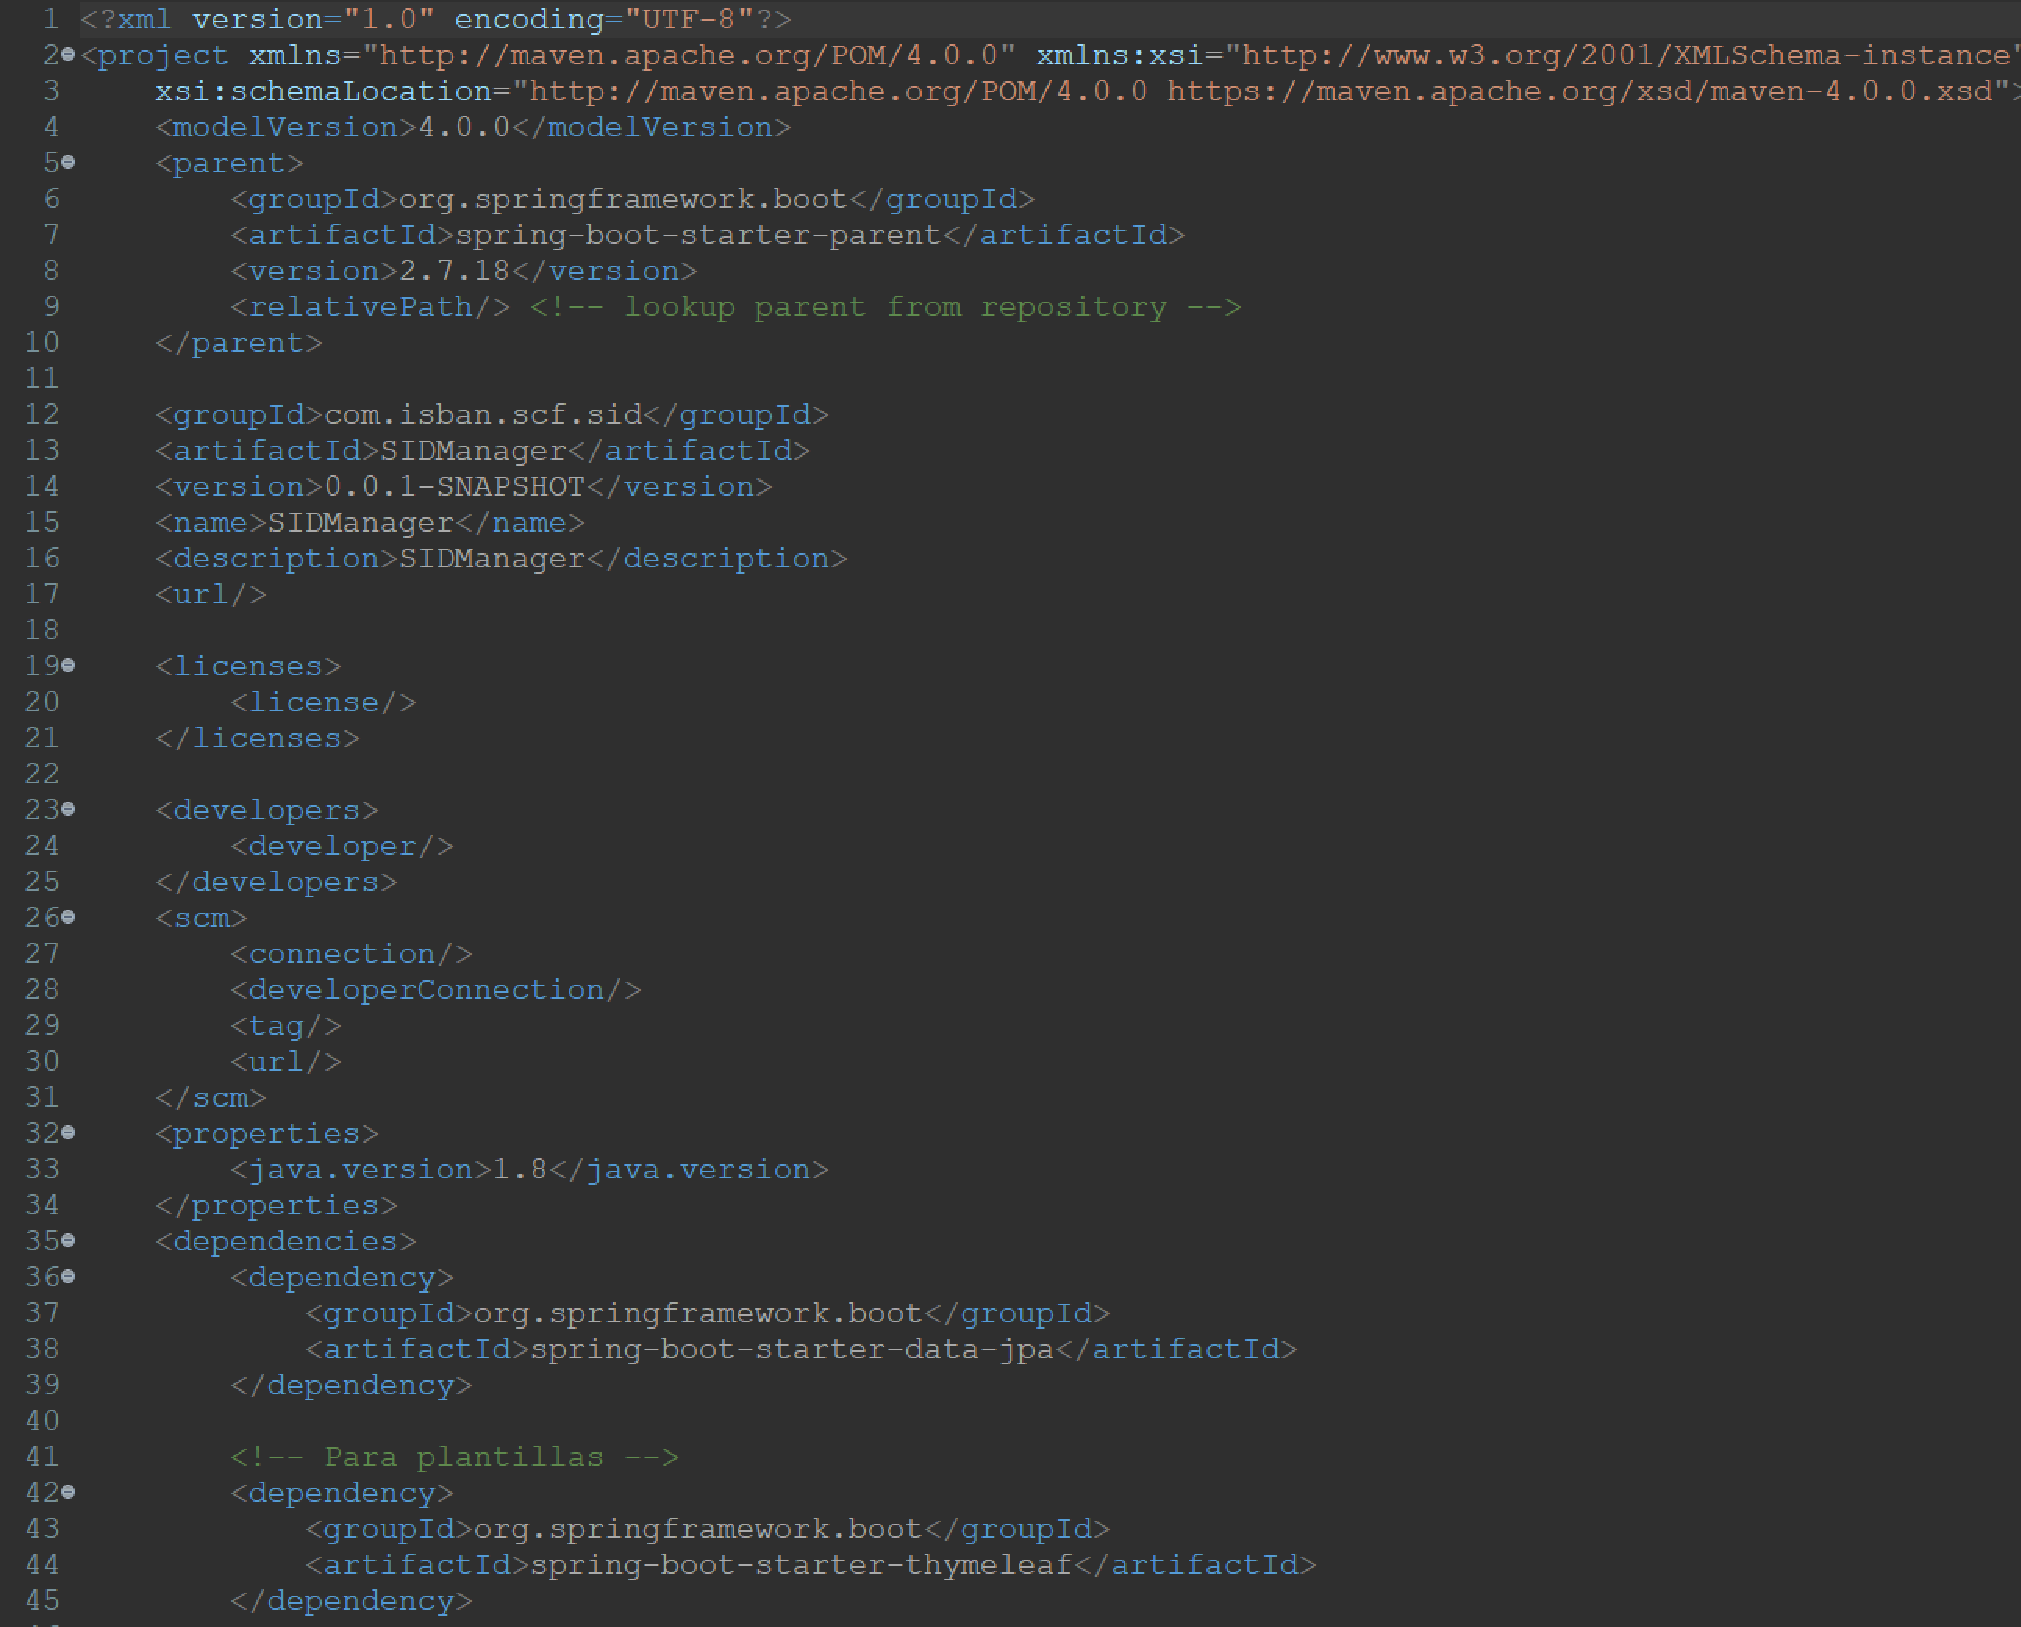
\includegraphics[width=0.75\linewidth]{imagenes/code/maven_pom_xml_example.pdf}
    \caption{Maven pom file example}
    \label{fig:maven_pom}
\end{figure}

\subsection{Dependencias principales}

A continuación, se describen las principales dependencias empleadas en el proyecto y su propósito:

\begin{enumerate}
    \item \textbf{Thymeleaf}:
    Thymeleaf es un motor de plantillas que permite integrar datos dinámicos en las vistas HTML. Su uso principal en el proyecto es la generación de las interfaces del usuario, facilitando la comunicación entre el frontend y el backend.

    \item \textbf{MySQL Connector}:
    Este conector es la biblioteca que permite la conexión entre la aplicación Java y la base de datos MySQL. Es fundamental para realizar operaciones de consulta, inserción, actualización y eliminación en la base de datos.

    \item \textbf{javax.mail}:
    Biblioteca utilizada para la implementación de funcionalidades de envío de correos electrónicos. En este proyecto, se emplea para enviar correos de confirmación a los usuarios registrados, asegurando una validación adecuada de sus cuentas.

    \item \textbf{Javadoc}:
    Javadoc es una herramienta incluida en el JDK que permite generar documentación de las clases y métodos del proyecto a partir de comentarios en el código fuente. Esto facilita la comprensión y el mantenimiento del sistema.

    \item \textbf{Log4j}:
    Log4j es una biblioteca para la gestión de registros (logs). Se utiliza para registrar eventos, errores y mensajes informativos durante la ejecución de la aplicación, lo que es crucial para depuración y monitorización.

\end{enumerate}



\section{ API de gestión de documentos}

Para poder hablar de la API, es importante hacer una distinción entre las dos partes principales de la aplicación: por un lado, la gestión de usuarios, y por otro, la gestión de documentos.

En este apartado, vamos a hablar de la gestión de documentos, es decir, de como funciona la aplicación por dentro para mostrar por pantalla el listado con las características de los documentos.

encontramos tres funciones principales en el controlador:


    \textbf{ \subsection{ Función getAllDocuments }}
    Esta función llama al método \texttt{getAllDocuments} del servicio \texttt{DocumentService} y devuelve la respuesta. El código de la función \texttt{getAllDocuments}, junto con sus logs asociados, es el siguiente:

    \begin{lstlisting}[language=Java]
@GetMapping()
public String getAllDocuments(Model model) {
    logger.debug(" ----- Entering getAllDocuments ----- ");
    model.addAttribute("documents", documentService.getAllDocuments());
    logger.debug(" ----- Exiting getAllDocuments ----- ");
    logger.debug(" ____________________________________ ");
    return "documentsView"; 
}
    \end{lstlisting}

    Una vez en el método \texttt{getAllDocuments} del \texttt{DocumentService}, este llama a la función \texttt{findAll} del \texttt{DocumentRepository}, que es el repositorio encargado de interactuar con la base de datos. El código es el siguiente:

    \begin{lstlisting}[language=Java]
public List<Document> getAllDocuments() {
    logger.debug(" Entering findAllDocuments ");
    return documentRepository.findAll();
}
    \end{lstlisting}

    Gracias a JPA, la sintaxis utilizada (\texttt{findAll}) permite generar automáticamente la consulta SQL sin necesidad de que el programador escriba la consulta explícitamente en el \texttt{DocumentRepository}. Esto no solo ahorra tiempo, sino que también reduce la posibilidad de errores y mejora la claridad del código. Para una mejor comprensión, se recomienda revisar la figura \ref{fig:jpa-usage}.

    Más adelante, en la sección \ref{sec:jpa-sintaxis}, se explicará con más detalle el uso de JPA.

    En resumen, esta función devuelve todos los documentos de la base de datos, sin restricciones ni filtros aplicados, junto con sus respectivos datos asociados (tal como se explicó en la sección de arquitectura de los documentos \ref{subsec:document-architecture}).

    
    \textbf { \subsection { Función getNotReceivedDocuments }}
    Esta función llama al método \texttt{getNotReceivedDocuments} del servicio \texttt{DocumentService} y devuelve la respuesta. El código de la función \texttt{getNotReceivedDocuments}, junto con sus logs asociados, es el siguiente:

    \begin{lstlisting}[language=Java]
@GetMapping("/not-received")
public String getNotReceivedDocuments(Model model) {
    logger.debug(" ----- Entering getNotReceivedDocuments ----- ");
    model.addAttribute("documents", documentService.getNotReceivedDocuments());
    model.addAttribute("isShowingUnsaveds", "Yes");
    logger.debug(" ----- Exiting getNotReceivedDocuments ----- ");
    
    return "documentsView";
}
    \end{lstlisting}

    Una vez en el método \texttt{getNotReceivedDocuments} del \texttt{DocumentService}, este llama a la función \texttt{findByReceivedAtIsNull} del \texttt{DocumentRepository}. El código es el siguiente:

    \begin{lstlisting}[language=Java]
public List<Document> getNotReceivedDocuments() {
    logger.debug(" Entering getNotReceivedDocuments ");
    return documentRepository.findByReceivedAtIsNull();
}
    \end{lstlisting}

    En resumen, esta función devuelve todos los documentos de la base de datos que no hayan sido guardados correctamente ya que no tienen fecha en el apartado \texttt{received\_at} (para más información sobre la arquitectura del documento ver la sección \ref{subsec:document-architecture}), por lo que no han sido recibidos. 

    
    \textbf { \subsection { Función listDocuments}}

La función \texttt{listDocuments} es una de las piezas clave de la aplicación, ya que se encarga de recuperar y filtrar los documentos almacenados en la base de datos según un intervalo de fechas. Esta función combina dos métodos principales del servicio \texttt{DocumentService}: \texttt{checkDates} y \texttt{getFilteredDocuments}. A continuación, se describe en detalle su funcionamiento y los componentes involucrados.

\textbf{Descripción de la función}

La función \texttt{listDocuments} realiza las siguientes tareas:

\begin{enumerate}
    \item \textbf{Validación y ajuste de fechas}: A través del método \texttt{checkDates}, se valida y ajusta el intervalo de fechas proporcionado por el usuario. Este intervalo se almacena en una clase auxiliar llamada \texttt{DateRange}, que encapsula las fechas de inicio y fin para facilitar su manejo entre métodos.

    \item \textbf{Filtrado de documentos}: Utilizando el intervalo de fechas validado, se invoca el método \texttt{getFilteredDocuments} para recuperar los documentos que cumplen con el criterio de filtrado.

    \item \textbf{Preparación de la respuesta}: Finalmente, la función añade al modelo (\texttt{model}) los documentos filtrados, junto con las fechas de inicio y fin utilizadas en el filtrado. Esta información se envía a la vista para su visualización.
\end{enumerate}

El código de la función \texttt{listDocuments}, junto con sus logs asociados, es el siguiente:

\begin{lstlisting}[language=Java]
@GetMapping("/list")
public String listDocuments(
        @RequestParam(value = "min-date",  required = false) String startDate,
        @RequestParam(value = "max-date", required = false) String endDate,
        Model model) throws Exception {
    logger.debug(" ----- Entering listDocuments ----- ");
    
    DateRange dateRange = documentService.checkDates(startDate, endDate, model);
    
    model.addAttribute("documents", 
            documentService.getFilteredDocuments(
                    dateRange.getStartDate(),
                    dateRange.getEndDate()
                    ));    	
    model.addAttribute("startDate", dateRange.getStartDate());
    model.addAttribute("endDate", dateRange.getEndDate());
    model.addAttribute("isShowingUnsaveds", "No");
    
    logger.debug(" ----- Exiting listDocuments ----- ");
    logger.debug(" ____________________________________ ");
        
    return "documentsView";
}
\end{lstlisting}

\textbf{Método \texttt{getFilteredDocuments}}

Una vez que el intervalo de fechas ha sido validado, la función \texttt{listDocuments} invoca el método \texttt{getFilteredDocuments} del servicio \texttt{DocumentService}. Este método, a su vez, llama a una función del repositorio \texttt{DocumentRepository} para ejecutar la consulta SQL que filtra los documentos según las fechas proporcionadas. El código es el siguiente:

\begin{lstlisting}[language=Java]
public List<Document> getFilteredDocuments(Date startDate, Date endDate) {
    logger.debug(" Entering getFilteredDocuments ");
    return documentRepository.findFilteredDocuments(startDate, endDate);
}
\end{lstlisting}

Dado que esta consulta es específica y no se ajusta a las convenciones automáticas de JPA, se ha implementado manualmente en el repositorio utilizando una anotación \texttt{@Query}. La consulta SQL correspondiente es la siguiente:

\begin{lstlisting}[language=Java]
@Query(value = "SELECT CLIENT_APP_ID, CLIENT_DOC_ID, PROVIDER_ID, SENT_AT, RECEIVED_AT"
            + " FROM documents WHERE SENT_AT > :startDate AND SENT_AT < :endDate", nativeQuery = true)
List<Document> findFilteredDocuments(@Param("startDate") Date startDate, @Param("endDate") Date endDate); 
\end{lstlisting}

\textbf{Método \texttt{checkDates}}

El método \texttt{checkDates} desempeña un papel crucial en la función \texttt{listDocuments}, ya que se encarga de validar y ajustar las fechas proporcionadas por el usuario. Su implementación responde a tres necesidades principales:

\begin{itemize}
    \item \textbf{Validación de errores}: Garantiza que las fechas proporcionadas sean válidas y estén en el formato correcto. Si no se realiza esta validación, errores en las fechas podrían interrumpir el funcionamiento de la aplicación.

    \item \textbf{Pseudopaginación}: En entornos de preproducción, se observó que la carga de más de 80 mil documentos podía tardar entre 6 y 8 minutos. Para optimizar el rendimiento, se implementó una pseudopaginación que limita el intervalo de fechas a un máximo de 10 días. Este límite se estableció tras un análisis exhaustivo que demostró que, a partir de este número, el tiempo de carga crecía exponencialmente.

    \item \textbf{Manejo de casos especiales}: El método gestiona situaciones en las que el usuario no proporciona ambas fechas o cuando el intervalo de fechas excede el límite establecido.
\end{itemize}

El código del método \texttt{checkDates} es el siguiente:

\begin{lstlisting}[language=Java]
public DateRange checkDates(String stringStartDate, String stringEndDate, Model model) {
    final int daysRange = 10;  
    DateRange dateRange;
    boolean isCorrectRange = true;
    
    try {
        if (DateUtils.checkDate(stringStartDate) && DateUtils.checkDate(stringEndDate)) {
            Date startDate = DateUtils.stringToUtilsDate(stringStartDate);
            Date endDate = DateUtils.stringToUtilsDate(stringEndDate);
            
            int daysBetween = DateUtils.daysBetween(startDate, endDate);
            
            if(daysBetween != -1 && daysBetween <= daysRange) {
                dateRange = new DateRange(startDate, endDate);
                logger.info(" Returning FILTERED documents ");
            } else {
                dateRange = new DateRange(-daysRange);
                
                logger.warn(" Exceded maximum day range ( " +
                            daysBetween + 
                            " ) with: " + 
                            daysRange);
                logger.warn(" Returning last 10 days ");
                
                isCorrectRange = false;
            }
        } else if (DateUtils.checkDate(stringEndDate)) {
            dateRange = new DateRange(DateUtils.stringToUtilsDate(stringEndDate), -daysRange);
            isCorrectRange = false;
        } else if (DateUtils.checkDate(stringStartDate)) {
            dateRange = new DateRange(DateUtils.stringToUtilsDate(stringStartDate), daysRange);
            isCorrectRange = false;
        } else {
            dateRange = new DateRange(-daysRange);
        }
    } catch (ParseException e) {
        logger.error(" ERROR in getFilteredDocuments: " + e);
        dateRange = new DateRange(-daysRange);			
    }
    
    if (!isCorrectRange) {
        model.addAttribute("responseMessage", ResponseEnum.LIST_WARNING_1.getMessageKey());
        model.addAttribute("isAWarningMessage", true);
    }
    
    return dateRange;
}
\end{lstlisting}

\textbf{Casos manejados por \texttt{checkDates}}

El método \texttt{checkDates} está diseñado para manejar cuatro escenarios principales:

\begin{itemize}
    \item \textbf{Ambas fechas proporcionadas}: Si las fechas son válidas y el intervalo no excede los 10 días, se devuelve el intervalo original. En caso contrario, se ajusta el intervalo a los últimos 10 días y se notifica al usuario.
    
    \item \textbf{Solo la fecha de fin proporcionada}: Se calcula un intervalo de 10 días hacia atrás a partir de la fecha de fin.
    
    \item \textbf{Solo la fecha de inicio proporcionada}: Se calcula un intervalo de 10 días hacia adelante a partir de la fecha de inicio.
    
    \item \textbf{Ninguna fecha proporcionada}: Se devuelve un intervalo predeterminado de los últimos 10 días.
    
    \item \textbf{Error en el formato de las fechas}: Si ocurre un error al parsear las fechas, se devuelve un intervalo predeterminado y se registra el error.
\end{itemize}

\textbf{Conclusión de listDocuments}

En resumen, la función \texttt{listDocuments} permite recuperar documentos filtrados por un intervalo de fechas, optimizando el rendimiento mediante la pseudopaginación y garantizando la robustez del sistema mediante la validación de entradas. Este enfoque no solo mejora la experiencia del usuario, sino que también asegura un manejo eficiente de grandes volúmenes de datos.


\section{ API de gestión de usuarios}
En lo que respecta a la gestión de usuarios, encontramos tres apartados principales (proceso de registro, inicio de sesión y cambio de contraseña) en los que se agrupan las distintas funciones del controlador ClientController. Estos apartados son:

% Sign Up
\textbf{ \subsection{ Proceso de registro (signup) }}
El proceso de registro en la aplicación SIDManager consta de tres pasos (o funciones). El primero es la carga de la página de registro, el segundo es el proceso de registrarse y el tercero es la confirmación del usuario a través del correo electrónico. Estos tres pasos se corresponden a tres funciones distintas: getCreateClientUserView, createClientUser, getConfirmation. Las funciones están detalladas a continuación:


\begin{enumerate}
    \item \textbf{ Función getCreateClientUserView} 

    
    Esta función devuelve la vista (o página) del proceso de registro del usuario. La función en el ClientController es:
\begin{lstlisting}[language=Java]
@GetMapping("/user/create")
public String getCreateClientUserView() {
    logger.debug("Entering GET: /user/create");
    
    return "createClientUserView"; 
}
\end{lstlisting}
    Esta función devuelve la vista ante la petición GET del usuario para poder comenzar el registro. Después de rellenar los campos del registro (correo electrónico, contraseña y contraseña repetida) con los datos del usuario y de pulsar el botón "sign up" se llama a la función createClientUser.
    

  \item \textbf{ Función createClientUser}

La función \texttt{createClientUser} es la encargada de gestionar el proceso de registro de un nuevo usuario en la aplicación. Esta función recibe los datos del formulario de registro, valida la información y, si todo es correcto, guarda el usuario en la base de datos y envía un correo electrónico de confirmación. A continuación, se describe su funcionamiento en detalle.

\begin{lstlisting}[language=Java]
@PostMapping("/user/create")
public String createClientUser(Model model, 
                                @ModelAttribute ClientUser clientUser,
                                @RequestParam("psw-repeat") String passwordRepeat
                                ) throws Exception {
    
    logger.debug(" - Entering clientUserService.createClientUser(), from POST: /user/create");
    
    ResponseEnum responseMessage = clientUserService.createClientUser(clientUser, passwordRepeat);

    model.addAttribute("responseMessage", responseMessage.getMessageKey());
    addColorToResponse(model, responseMessage);
    
    return "createClientUserView";  
}
\end{lstlisting}

\begin{enumerate}
    \item \textbf{Parámetros de entrada}:
    \begin{itemize}
        \item \texttt{Model model}: Se utiliza para pasar datos a la vista, como mensajes de respuesta o errores.
        \item \texttt{@ModelAttribute ClientUser clientUser}: Contiene los datos del usuario proporcionados en el formulario de registro (correo electrónico y contraseña).
        \item \texttt{@RequestParam("psw-repeat") String passwordRepeat}: Contiene la contraseña repetida para verificar que coincida con la contraseña original.
    \end{itemize}

    \item \textbf{Lógica del controlador}:
    \begin{itemize}
        \item La función llama al método \texttt{createClientUser} del servicio \texttt{ClientUserService}, pasando los datos del usuario y la contraseña repetida.
        \item Dependiendo del resultado del servicio, se añade un mensaje de respuesta al modelo (\texttt{model}) para informar al usuario sobre el éxito o el fracaso del registro.
        \item Finalmente, se devuelve la vista \texttt{createClientUserView}, que muestra el formulario de registro junto con el mensaje de respuesta.
    \end{itemize}
\end{enumerate}

     \item \textbf{ Función \texttt{saveClientUser}}

La función \texttt{saveClientUser} es la encargada de guardar un nuevo usuario en la base de datos. Esta función realiza varias operaciones críticas, como la encriptación de la contraseña, la generación de un código de confirmación único y la asignación de un estado inicial al usuario. A continuación, se describe su funcionamiento en detalle.

\begin{lstlisting}[language=Java]
@Transactional
public ClientUser saveClientUser(ClientUser clientUser) throws Exception {
    try {
        if (clientUser.getPassword() != null) {
            logger.debug(" -- Entering encryptMessage()");
            clientUser.setPassword(encryptFacade(clientUser.getPassword()));
            
            logger.debug(" -- Entering randomAlphanumeric()");
            clientUser.setConfirmationCode(RandomStringUtils.randomAlphanumeric(30));
            
            clientUser.setStatus(0);
            clientUser.setCreationDate(new Date()); 
            clientUserRepository.save(clientUser);
        } else {
             throw new IllegalArgumentException("Password cannot be null");
        }
    } catch (Exception e) {
        logger.error(" ERROR: Possible error in encryption, confirmation code generation "
                + " or saveClientUser:" + e);
        throw e;
    }
    
    return clientUser;
}
\end{lstlisting}

\begin{enumerate}
    \item \textbf{Encriptación de la contraseña}:
    \begin{itemize}
        \item La contraseña proporcionada por el usuario se encripta utilizando la función \texttt{encryptFacade}. Esto garantiza que la contraseña no se almacene en texto plano en la base de datos, mejorando la seguridad del sistema. Para más información sobre la ecriptación ver la sección \ref{subsec:cryptography}.
    \end{itemize}

    \item \textbf{Generación del código de confirmación}:
    \begin{itemize}
        \item Se genera un código de confirmación único utilizando \texttt{RandomStringUtils.randomAlphanumeric(30)}. Este código se enviará al usuario por correo electrónico y se utilizará para confirmar su registro.
    \end{itemize}

    \item \textbf{Asignación del estado inicial}:
    \begin{itemize}
        \item El estado del usuario se establece en \texttt{0}, lo que indica que el usuario ha sido creado pero aún no ha confirmado su correo electrónico. Mientras tenga su estado en 0 no podrá iniciar sesión, por lo que tendrá que confirmar el usuario abriendo el correo con el enlace proporcionado para ello.
    \end{itemize}

    \item \textbf{Fecha de creación}:
    \begin{itemize}
        \item Se registra la fecha y hora actuales como la fecha de creación del usuario.
    \end{itemize}

    \item \textbf{Guardado en la base de datos}:
    \begin{itemize}
        \item Finalmente, el usuario se guarda en la base de datos utilizando el método \texttt{save} del repositorio \texttt{clientUserRepository}.
    \end{itemize}

    \item \textbf{Manejo de excepciones}:
    \begin{itemize}
        \item Si ocurre algún error durante el proceso (por ejemplo, si la contraseña es nula), se lanza una excepción y se registra el error en los logs.
    \end{itemize}
\end{enumerate}

\textbf{Integración en el proceso de registro}

Las funciones explicadas anteriormente trabajan juntas para garantizar un proceso de registro seguro y eficiente:

\begin{enumerate}
    \item \textbf{Validación de datos}:
    \begin{itemize}
        \item La función \texttt{createClientUser} valida que las contraseñas coincidan y que el correo electrónico no esté ya registrado en la base de datos.
    \end{itemize}

    \item \textbf{Guardado seguro del usuario}:
    \begin{itemize}
        \item La función \texttt{saveClientUser} se encarga de encriptar la contraseña, generar un código de confirmación único y guardar el usuario en la base de datos.
    \end{itemize}

    \item \textbf{Confirmación por correo electrónico}:
    \begin{itemize}
        \item Una vez que el usuario se ha guardado correctamente, se envía un correo electrónico con el código de confirmación para que el usuario pueda activar su cuenta.
    \end{itemize}

    \item \textbf{Retroalimentación al usuario}:
    \begin{itemize}
        \item El controlador devuelve un mensaje de respuesta a la vista, informando al usuario sobre el éxito o el fracaso del registro.
    \end{itemize}
\end{enumerate}

\textbf{Conclusión registro}

Las funciones comentadas son fundamentales para el proceso de registro en la aplicación SIDManager. Juntas, garantizan que los datos del usuario se validen, almacenen de manera segura y se confirmen a través de un correo electrónico. Este enfoque no solo mejora la seguridad del sistema, sino que también proporciona una experiencia de usuario fluida y confiable.
    
    \item \textbf{Función getConfirmation}

Antes de explicar la función \texttt{getConfirmation}, es importante recordar que un usuario, al crearse, tiene un estado inicial de \texttt{0} (creado pero no confirmado). Para confirmar su cuenta, se le envía un correo electrónico con un enlace único que lo redirige a una página de confirmación. Esta página cambia su estado a \texttt{1} (confirmado) una vez que el usuario accede al enlace. La función \texttt{getConfirmation} en el \texttt{UserController} es la encargada de gestionar este proceso.

\textbf{Código de la función \texttt{getConfirmation}}

\begin{lstlisting}[language=Java]
@GetMapping("/user/confirm")
public String getConfirmation(Model model, 
                              @RequestParam("email") String email,
                              @RequestParam("confirmationCode") String confirmationCode) {
    
    logger.debug(" - Entering clientUserService.confirmUser(), from GET: /user/confirm");
    ResponseEnum responseMessage = clientUserService.confirmUser(email, confirmationCode);
    logger.debug(" - Exiting clientUserService.confirmUser()");
    
    model.addAttribute("responseMessage", responseMessage.getMessageKey());
    addColorToResponse(model, responseMessage);
    
    return "confirmationUser"; 
}    
\end{lstlisting}

\textbf{Explicación del código \texttt{getConfirmation}}

\begin{enumerate}
    \item \textbf{Parámetros de entrada}:
    \begin{itemize}
        \item \textbf{Model model}: Se utiliza para pasar datos a la vista, como mensajes de respuesta o errores.
        \item \textbf{@RequestParam(''email'') String email}: Contiene el correo electrónico del usuario que se está confirmando.
        \item \textbf{@RequestParam(''confirmationCode'') String confirmationCode}: Contiene el código de confirmación único asociado al usuario.
    \end{itemize}

    \item \textbf{Lógica del controlador}:
    \begin{itemize}
        \item La función llama al método \texttt{confirmUser} del servicio \texttt{ClientUserService}, pasando el correo electrónico y el código de confirmación.
        \item Dependiendo del resultado del servicio, se añade un mensaje de respuesta al modelo (\texttt{model}) para informar al usuario sobre el éxito o el fracaso de la confirmación.
        \item Finalmente, se devuelve la vista \texttt{confirmationUser}, que muestra el resultado de la confirmación.
    \end{itemize}
\end{enumerate}

\textbf{Código de la función \texttt{confirmUser}}

\begin{lstlisting}[language=Java]
@Transactional
public ResponseEnum confirmUser(String email,
                                String confirmationCode
                                ) {
    ResponseEnum responseMessage;
    ClientUser clientUser = clientUserRepository.findByEmailAndConfirmationCodeAndStatus(email, confirmationCode, 0);	
    
    if (clientUser != null) {
        responseMessage = ResponseEnum.CONFIRM_SUCCESS;
        clientUser.setStatus(1);
        clientUser.setConfirmationDate(new Date()); 
        clientUserRepository.save(clientUser);
    } else {
        logger.debug(" User not found, not correct or already confirmed. ");
        responseMessage = ResponseEnum.CONFIRM_WARNING;
    }
    
    return responseMessage;
}
\end{lstlisting}

\textbf{Explicación del código \texttt{confirmUser}}

\begin{enumerate}
    \item \textbf{Búsqueda del usuario}:
    \begin{itemize}
        \item Se busca en la base de datos un usuario que coincida con el correo electrónico, el código de confirmación y tenga un estado de \texttt{0} (no confirmado). Esto se realiza mediante la función \texttt{findByEmailAndConfirmationCodeAndStatus} del repositorio \texttt{clientUserRepository}.
    \end{itemize}

    \item \textbf{Confirmación del usuario}:
    \begin{itemize}
        \item Si se encuentra un usuario que cumple con los criterios, se cambia su estado a \texttt{1} (confirmado) y se registra la fecha y hora de confirmación.
        \item El usuario actualizado se guarda en la base de datos utilizando el método \texttt{save} del repositorio.
        \item Se devuelve un mensaje de éxito (\texttt{ResponseEnum.CONFIRM\_SUCCESS}).
    \end{itemize}

    \item \textbf{Manejo de errores}:
    \begin{itemize}
        \item Si no se encuentra un usuario que cumpla con los criterios (por ejemplo, si el usuario ya está confirmado o el código de confirmación es incorrecto), se devuelve un mensaje de advertencia (\texttt{ResponseEnum.CONFIRM\_WARNING}).
    \end{itemize}
\end{enumerate}

La función \texttt{getConfirmation} y su correspondiente método en el servicio, \texttt{confirmUser}, trabajan juntos para garantizar que el proceso de confirmación del usuario sea seguro y eficiente:

\begin{enumerate}
    \item \textbf{Acceso al enlace de confirmación}:
    \begin{itemize}
        \item El usuario accede al enlace único enviado por correo electrónico, que contiene su correo electrónico y código de confirmación.
    \end{itemize}

    \item \textbf{Validación del usuario}:
    \begin{itemize}
        \item El sistema verifica que el correo electrónico y el código de confirmación coincidan con un usuario no confirmado en la base de datos.
    \end{itemize}

    \item \textbf{Confirmación y actualización}:
    \begin{itemize}
        \item Si la validación es exitosa, el estado del usuario se cambia a \texttt{1} (confirmado) y se registra la fecha de confirmación.
    \end{itemize}

    \item \textbf{Retroalimentación al usuario}:
    \begin{itemize}
        \item El sistema muestra un mensaje en la vista \texttt{confirmationUser} para informar al usuario sobre el resultado del proceso.
    \end{itemize}
\end{enumerate}

\textbf{Conclusión getConfirmation}

La función \texttt{getConfirmation} y su método asociado \texttt{confirmUser} son fundamentales para completar el proceso de registro en la aplicación SIDManager. Juntos, garantizan que solo los usuarios que hayan verificado su correo electrónico puedan activar sus cuentas, lo que mejora la seguridad y la confiabilidad del sistema. Este enfoque también proporciona una experiencia de usuario fluida, ya que el proceso de confirmación es rápido y sencillo.

\end{enumerate}
    

% Login
\subsection{Inicio de sesión (login)}

El proceso de inicio de sesión en la aplicación SIDManager es una de las funcionalidades más críticas, ya que garantiza que solo los usuarios autorizados puedan acceder al sistema. Inicialmente, este proceso se implementó de manera manual, pero debido a consideraciones de seguridad, se migró a una solución basada en \textbf{Spring Boot Security}. A continuación, se describe la función \texttt{getLoginView}, que se encarga de cargar la vista de inicio de sesión.

\textbf{Función getLoginView}

La función \texttt{getLoginView} es la encargada de preparar y devolver la vista de inicio de sesión. Esta función configura las URLs necesarias para acciones como la recuperación de contraseña y el registro de nuevos usuarios, además de manejar mensajes de error que puedan haberse generado en intentos previos de inicio de sesión.

\textbf{Código de la función}

\begin{lstlisting}[language=Java]
@GetMapping("/user/login")
public String getLoginView(Model model,
                           HttpServletRequest request
                           ) throws Exception {
    String serverUrl = SharedProperties.get("serverUrl");
    String requestUpdatePasswordUrl =  serverUrl + "user/requestUpdatePassword";
    String createClientUserUrl = serverUrl + "user/create";
    String errorMessage = (String) request.getSession().getAttribute("error");
    
    model.addAttribute("requestUpdatePasswordUrl", requestUpdatePasswordUrl);
    model.addAttribute("createClientUserUrl", createClientUserUrl);
    
    if (errorMessage != null) {
        ResponseEnum responseMessage = ResponseEnum.LOGIN_WARNING_1;
        model.addAttribute("responseMessage", responseMessage.getMessageKey());
        addColorToResponse(model, responseMessage);
        
        // Elimina el mensaje de error de la sesión
        request.getSession().removeAttribute("error");
    }
    
    return "loginView";
}
\end{lstlisting}

\textbf{Explicación del código}

\begin{enumerate}
    \item \textbf{Parámetros de entrada}:
    \begin{itemize}
        \item \texttt{Model model}: Se utiliza para pasar datos a la vista, como URLs y mensajes de error.
        \item \texttt{HttpServletRequest request}: Permite acceder a la sesión del usuario y recuperar atributos almacenados, como mensajes de error.
    \end{itemize}

    \item \textbf{Configuración de URLs}:
    \begin{itemize}
        \item Se obtiene la URL base del servidor (\texttt{serverUrl}) desde las propiedades compartidas (\texttt{SharedProperties}).
        \item Se construyen las URLs para la recuperación de contraseña (\texttt{requestUpdatePasswordUrl}) y el registro de nuevos usuarios (\texttt{createClientUserUrl}).
        \item Estas URLs se añaden al modelo para que estén disponibles en la vista.
    \end{itemize}

    \item \textbf{Manejo de mensajes de error}:
    \begin{itemize}
        \item Se verifica si hay un mensaje de error almacenado en la sesión del usuario (\texttt{request.getSession().getAttribute("error")}).
        \item Si existe un mensaje de error, se añade al modelo para mostrarlo en la vista. Además, se elimina el mensaje de la sesión para evitar que se muestre en futuras cargas de la página.
    \end{itemize}

    \item \textbf{Retorno de la vista}:
    \begin{itemize}
        \item La función devuelve la vista \texttt{loginView}, que muestra el formulario de inicio de sesión junto con las URLs configuradas y los mensajes de error, si los hay.
    \end{itemize}
\end{enumerate}

\textbf{Integración con Spring Boot Security}

En lo que respecta al proceso de inicio de sesión, en la primera versión se implementó manualmente, pero por cuestiones de seguridad se cambió a un inicio de sesión implementado con Spring Boot Security. Por tanto, si quiere saber más del login consulte la sección \ref{sec:login}.

\textbf{Conclusión de inicio de sesión}

La función \texttt{getLoginView} es esencial para cargar la vista de inicio de sesión y configurar los elementos necesarios, como las URLs de recuperación de contraseña y registro. Además, maneja mensajes de error para mejorar la experiencia del usuario. La migración a Spring Boot Security ha fortalecido la seguridad del proceso de inicio de sesión, garantizando que solo los usuarios autorizados puedan acceder al sistema de manera segura.

% Update psw
\subsection{Cambio de contraseña (update password)}
\label{subsec:update-password}

El proceso de cambio de contraseña en la aplicación SIDManager es una funcionalidad crítica que garantiza la seguridad de los usuarios al permitirles actualizar sus credenciales de acceso. Este proceso consta de cuatro pasos principales, cada uno implementado mediante funciones específicas en el controlador y el servicio. A continuación, se describen en detalle estas funciones y su funcionamiento.

\begin{enumerate}

    \item \textbf{  Función getRequestUpdatePasswordView}

La función \textbf{getRequestUpdatePasswordView} es la encargada de cargar la vista donde el usuario puede solicitar un cambio de contraseña. Esta vista incluye un formulario para ingresar el correo electrónico asociado a la cuenta.

\begin{lstlisting}[language=Java]
@GetMapping("/user/requestUpdatePassword")
public String getRequestUpdatePasswordView() {
    return "requestUpdatePasswordView";
}
\end{lstlisting}

\textbf{Explicación del código}
\begin{itemize}
    \item La función responde a una solicitud HTTP GET en la ruta \textbf{/user/requestUpdatePassword}.
    \item Devuelve la vista \textbf{requestUpdatePasswordView}, que contiene el formulario para solicitar el cambio de contraseña.
\end{itemize}

    \item \textbf{Función requestUpdatePassword}

Una vez que el usuario ingresa su correo electrónico y envía el formulario, se invoca la función \textbf{requestUpdatePassword}. Esta función valida el correo electrónico y, si es válido, envía un enlace único al usuario para que pueda cambiar su contraseña.

\begin{lstlisting}[language=Java]
@PostMapping("user/requestUpdatePassword")
public String requestUpdatePassword(Model model,
        @RequestParam("email") String email
        ) throws Exception  {
    
    ResponseEnum responseMessage = clientUserService.sendUpdatePasswordUrl(email);
    
    model.addAttribute("responseMessage", responseMessage.getMessageKey());
    addColorToResponse(model, responseMessage);
    
    return "requestUpdatePasswordView";
}
\end{lstlisting}

\textbf{Explicación del código}
\begin{itemize}
    \item La función responde a una solicitud HTTP POST en la ruta \textbf{/user/requestUpdatePassword}.
    \item Recibe el correo electrónico del usuario como parámetro.
    \item Llama al método \textbf{sendUpdatePasswordUrl} del servicio \textbf{ClientUserService} para validar el correo electrónico y enviar el enlace de cambio de contraseña.
    \item Añade un mensaje de respuesta al modelo para informar al usuario sobre el resultado de la operación.
    \item Devuelve la vista \textbf{requestUpdatePasswordView} para mostrar el mensaje de respuesta.
\end{itemize}

\textbf{Método sendUpdatePasswordUrl}

El método \textbf{sendUpdatePasswordUrl} es el encargado de generar y enviar el enlace de cambio de contraseña al correo electrónico del usuario.

\begin{lstlisting}[language=Java]
public ResponseEnum sendUpdatePasswordUrl(String email) throws Exception {
    ResponseEnum responseMessage;
    ClientUser clientUser = clientUserRepository.findByEmail(email);
    
    if (clientUser != null && clientUser.getStatus() == 1) {
        String path = "user/updatePassword?email=";
        String urlUpdatePassword = this.getConfirmationUrl(clientUser, path);
        
        logger.debug(" - Entering sendMail");
        String subject = " Change the password of your SIDManager user. ";
        String body = " Click on the next URL if you want to change your password: ";
        Mail.sendMail(clientUser.getEmail(), urlUpdatePassword, subject, body);
        logger.debug(" - Exiting sendMail");
        
        responseMessage = ResponseEnum.UPDATE_PSW_SUCCESS_1;
    } else {
        responseMessage = ResponseEnum.UPDATE_PSW_WARNING_1;
        logger.info(" The user does not exist or is not confirmed. ");
    }

    return responseMessage;
}
\end{lstlisting}

\textbf{Explicación del código}
\begin{itemize}
    \item Busca al usuario en la base de datos utilizando el correo electrónico proporcionado.
    \item Si el usuario existe y está confirmado (estado \textbf{1}), genera un enlace único utilizando el método \textbf{getConfirmationUrl}.
    \item Envía el enlace al correo electrónico del usuario utilizando la clase \textbf{Mail} con su titulo, cuerpo del correo y enlace (para más información sobre el funcionamiento de la clase Mail ver \ref{subsec:mail}).
    \item Devuelve un mensaje de éxito o advertencia dependiendo del resultado de la operación.
\end{itemize}

\textbf{Método getConfirmationUrl}

El método \textbf{getConfirmationUrl} genera la URL de confirmación o cambio de contraseña utilizando la URL base del servidor y los datos del usuario.

\begin{lstlisting}[language=Java]
private String getConfirmationUrl(ClientUser clientUser,
      String path
      ) throws Exception {
    StringBuilder confirmationUrl = new StringBuilder();
    String serverUrl = SharedProperties.get("serverUrl");
    
    confirmationUrl.append(serverUrl);
    confirmationUrl.append(path);
    confirmationUrl.append(clientUser.getEmail());
    confirmationUrl.append("&confirmationCode=");
    confirmationUrl.append(clientUser.getConfirmationCode());
    
    return confirmationUrl.toString();
}
\end{lstlisting}

\textbf{Explicación del código}
\begin{itemize}
    \item Construye una URL utilizando la URL base del servidor, el correo electrónico del usuario y su código de confirmación.
    \item La URL base se obtiene de las propiedades compartidas (\textbf{SharedProperties}), lo que permite cambiar la URL fácilmente sin modificar el código (para más información sobre la clase SharedProperties ver \ref{subsec:shared-properties}).
\end{itemize}

    \item \textbf{Función getUpdatePasswordView}

Cuando el usuario accede al enlace de cambio de contraseña, se invoca la función \textbf{getUpdatePasswordView}. Esta función valida el enlace y carga la vista para cambiar la contraseña.

\begin{lstlisting}[language=Java]
@GetMapping("/user/updatePassword")
public String getUpdatePasswordView(Model model, 
        HttpSession session,
        @RequestParam("email") String email,
        @RequestParam("confirmationCode") String confirmationCode
        ) throws Exception {
    boolean shouldFormBeShown = false;
    ResponseEnum responseMessage = clientUserService.getUpdatePasswordView(email, confirmationCode);
    
    if (responseMessage.getStatus() == ResponseEnum.UPDATE_PSW_SUCCESS_2.getStatus()) {
        shouldFormBeShown = true;
    } else {
        model.addAttribute("responseMessage", responseMessage.getMessageKey());
        addColorToResponse(model, responseMessage);
    }
    
    model.addAttribute("shouldFormBeShown", shouldFormBeShown);
    
    //Save the email to send it later in the post
    session.setAttribute("email", email);
    
    return "updatePasswordView";
}
\end{lstlisting}

\textbf{Explicación del código}
\begin{itemize}
    \item Valida el correo electrónico y el código de confirmación utilizando el método \textbf{getUpdatePasswordView} del servicio.
    \item Si la validación es exitosa, muestra el formulario para cambiar la contraseña.
    \item Si la validación falla, muestra un mensaje de error.
    \item Almacena el correo electrónico en la sesión para su uso posterior (ya que la función updatePassword lo necesita).
\end{itemize}

\textbf{Método getUpdatePasswordView}

El método \textbf{getUpdatePasswordView} valida que el usuario exista y que el código de confirmación sea correcto.

\begin{lstlisting}[language=Java]
public ResponseEnum getUpdatePasswordView(String email,
                                          String confirmationCode
                                          ) {
    ResponseEnum responseMessage;
    ClientUser clientUser 
        = clientUserRepository.findByEmailAndConfirmationCodeAndStatus(
                email, confirmationCode, 1);	

    if (clientUser != null) {
        responseMessage = ResponseEnum.UPDATE_PSW_SUCCESS_2;
    } else {
        responseMessage = ResponseEnum.UPDATE_PSW_WARNING_2;
        logger.info(responseMessage.getMessageKey());
    }
    
    return responseMessage;
}
\end{lstlisting}

\textbf{Explicación del código}
\begin{itemize}
    \item Busca al usuario en la base de datos utilizando el correo electrónico, el código de confirmación y el estado \textbf{1} (confirmado) usando la sintaxis de JPA.
    \item Devuelve un mensaje de éxito o advertencia dependiendo del resultado de la búsqueda.
\end{itemize}

    \item \textbf{Función updatePassword}

Finalmente, cuando el usuario envía el formulario de cambio de contraseña, se invoca la función \textbf{updatePassword}. Esta función valida las nuevas contraseñas y actualiza la contraseña en la base de datos.

\begin{lstlisting}[language=Java]
@PostMapping("/user/updatePassword")
    public String updatePassword( Model model,
              HttpSession session,
              @ModelAttribute ClientUser clientUser,
              @RequestParam("psw-repeat") String passwordRepeat
              ) throws Exception {
        String loginUrl = SharedProperties.get("serverUrl") + "user/login";
        String email = (String) session.getAttribute("email");
        boolean shouldFormBeShown = true;
        ResponseEnum responseMessage = clientUserService.updatePassword(email, clientUser, passwordRepeat);
    	
        if (responseMessage.getStatus() == ResponseEnum.UPDATE_PSW_SUCCESS_3.getStatus()) {
            shouldFormBeShown = false;
            model.addAttribute("loginUrl", loginUrl);
        } 
    	
        model.addAttribute("responseMessage", responseMessage.getMessageKey());
        model.addAttribute("shouldFormBeShown", shouldFormBeShown);
        addColorToResponse(model, responseMessage);
        
        return "updatePasswordView";
    }
\end{lstlisting}

\textbf{Explicación del código}
\begin{itemize}
    \item Recibe las nuevas contraseñas y valida que coincidan.
    \item Llama al método \textbf{updatePassword} del servicio para actualizar la contraseña en la base de datos.
    \item Muestra un mensaje de éxito o error y redirige al usuario a la página de inicio de sesión si la operación es exitosa.
\end{itemize}

\textbf{Método updatePassword}

El método \textbf{updatePassword} realiza la actualización de la contraseña en la base de datos.

\begin{lstlisting}[language=Java]
public ResponseEnum updatePassword(String email, 
           ClientUser clientUser, 
           String passwordRepeat
           ) throws Exception {
		ResponseEnum responseMessage;
		String password = clientUser.getPassword();
		
		 if (password != null && password.equals(passwordRepeat)) {
	        	// Check if the user exists in the database
		        ClientUser existingUser = this.getClientUser(email);
		        
		        if (existingUser != null) {
		        	existingUser.setPassword(encryptFacade(password));
		        	clientUserRepository.save(existingUser);
		            
		            responseMessage = ResponseEnum.UPDATE_PSW_SUCCESS_3;
		        } else {
		        	responseMessage = ResponseEnum.UPDATE_PSW_WARNING_4;
		        }
	        } else {
	        	responseMessage = ResponseEnum.UPDATE_PSW_WARNING_3;
	        }      
		
		return responseMessage;
	}
\end{lstlisting}

\textbf{Explicación del código}
\begin{itemize}
    \item Valida que las contraseñas coincidan y que el usuario exista en la base de datos.
    \item Encripta la nueva contraseña y la guarda en la base de datos.
    \item Devuelve un mensaje de éxito o error dependiendo del resultado de la operación.
\end{itemize}

\textbf{Conclusión cambio de contrasña}

El proceso de cambio de contraseña en SIDManager es un ejemplo de cómo se puede implementar una funcionalidad crítica de manera segura y eficiente. Utilizando Spring Boot y buenas prácticas de desarrollo, se garantiza que los usuarios puedan actualizar sus credenciales de manera sencilla y segura, protegiendo así la integridad de sus cuentas.

\end{enumerate}

\section{ Acceso a la base de datos }
\subsection{ Generación automática de consultas SQL con JPA }
\label{sec:jpa-sintaxis}
En esta sección se explicará cómo JPA (Java Persistence API) construye automáticamente consultas SQL a partir de su propia sintaxis, simplificando enormemente la interacción con la base de datos. Para ilustrar este proceso, nos basaremos en el ejemplo mostrado en la figura \ref{fig:jpa-usage}, donde se utiliza el método \texttt{findAll()}. Sin embargo, esto puede plantear una pregunta importante: ¿cómo sabe JPA que debe recuperar entidades de tipo \texttt{Document} y no de otra entidad de la base de datos?

La respuesta reside en la configuración de la clase \texttt{DocumentRepository}, que actúa como interfaz entre la capa de persistencia y la lógica de negocio. A continuación, se muestra el fragmento de código clave:

\begin{lstlisting}[language=Java]
import com.isban.scf.sid.model.Document;

@Repository
public interface DocumentRepository extends JpaRepository<Document, Long> {
\end{lstlisting}

\textbf{Explicación del código}

\begin{enumerate}
\item \textbf{Importación del modelo \texttt{Document}}:
En la primera línea del código, se importa la clase \texttt{Document}, que representa la entidad de la base de datos con la que se va a trabajar. Esta clase está anotada con \texttt{@Entity} en su definición, lo que indica a JPA que se trata de una entidad persistente mapeada a una tabla en la base de datos.

\item \textbf{Uso de la anotación \texttt{@Repository}}: 
La anotación \texttt{@Repository} marca la interfaz \texttt{DocumentRepository} como un componente de Spring encargado de la gestión de operaciones de persistencia. Esta anotación no solo permite que Spring detecte automáticamente esta clase durante el escaneo de componentes, sino que también proporciona manejo de excepciones específicas de persistencia.

\item \textbf{Extensión de \texttt{JpaRepository}}: 
La interfaz \texttt{DocumentRepository} extiende \texttt{JpaRepository<Document, Long>}, lo que le proporciona acceso a una serie de métodos predefinidos para realizar operaciones CRUD (Crear, Leer, Actualizar y Eliminar) sobre la entidad \texttt{Document}. El primer parámetro genérico (\texttt{Document}) indica el tipo de entidad con la que se trabajará, mientras que el segundo parámetro (\texttt{Long}) especifica el tipo de la clave primaria de dicha entidad.

\item \textbf{Generación automática de consultas}: 
Al extender \texttt{JpaRepository}, JPA automáticamente implementa métodos como \texttt{findAll()}, \texttt{findById()}, \texttt{save()}, entre otros, sin necesidad de escribir código adicional. En el caso de \texttt{findAll()}, JPA genera la consulta SQL necesaria para recuperar todos los registros de la tabla asociada a la entidad \texttt{Document}. Esto es posible gracias a la información proporcionada por los parámetros genéricos y las anotaciones de la entidad.

\end{enumerate}


\textbf{El modelo Document}

El modelo \texttt{Document} es una clase Java que representa la entidad \textbf{documentos} en la base de datos. Esta clase está mapeada a la tabla \texttt{documents} mediante anotaciones de JPA, lo que permite a JPA realizar operaciones de persistencia de manera automática. A continuación, se muestra el código de la clase \texttt{Document}:

\begin{lstlisting}[language=Java]
package com.isban.scf.sid.model;

import javax.persistence.Column;
import javax.persistence.Entity;
import javax.persistence.Id;
import javax.persistence.Table;

@Entity
@Table(name = "documents") // Nombre de la tabla en la base de datos
public class Document {
@Id
@Column(name = "CLIENT_DOC_ID")
private Long clientDocId; 

@Column(name = "CLIENT_APP_ID")
private Long clientAppId; 

@Column(name = "PROVIDER_ID")
private String providerId; 

@Column(name = "SENT_AT")
private String sentAt;

@Column(name = "RECEIVED_AT")
private String receivedAt;

// Getters y setters
public Long getClientDocId() {
    return clientDocId;
}

public void setClientDocId(Long clientDocId) {
    this.clientDocId = clientDocId;
}

public Long getClientAppId() {
    return clientAppId;
}

public void setClientAppId(Long clientAppId) {
    this.clientAppId = clientAppId;
}

public String getProviderId() {
    return providerId;
}

public void setProviderId(String providerId) {
    this.providerId = providerId;
}

public String getSentAt() {
    return sentAt;
}

public void setSentAt(String sentAt) {
    this.sentAt = sentAt;
}

public String getReceivedAt() {
    return receivedAt;
}

public void setReceivedAt(String receivedAt) {
    this.receivedAt = receivedAt;
}

\end{lstlisting}

\textbf{Explicación del modelo Document}

\begin{enumerate}
\item \textbf{Anotación \texttt{@Entity}}:
Esta anotación indica que la clase \texttt{Document} es una entidad JPA, lo que significa que está mapeada a una tabla en la base de datos.

\item \textbf{Anotación \texttt{@Table}}: 
La anotación \texttt{@Table(name = "documents")} especifica el nombre de la tabla en la base de datos a la que está asociada esta entidad. En este caso, la tabla se llama \texttt{documents}.

\item \textbf{Campo \texttt{clientDocId}}: 
Este campo está anotado con \texttt{@Id} y \texttt{@Column(name = ``CLIENT\_DOC\_ID``)}. El tipo de dato es \texttt{Long}, y su valor identifica de manera única cada documento en la base de datos.

\item \textbf{Campo \texttt{clientAppId}}: 
Este campo está anotado con \texttt{@Column(name = ``CLIENT\_APP\_ID``)} y representa el identificador de la aplicación cliente que creó el documento. Su tipo de dato es \texttt{Long}.

\item \textbf{Campo \texttt{providerId}}: 
Este campo está anotado con \texttt{@Column(name = ``PROVIDER\_ID``)} y almacena el identificador del proveedor que procesa el documento. Su tipo de dato es \texttt{String}.

\item \textbf{Campos \texttt{sentAt} y \texttt{receivedAt}}: 

Estos campos están anotados con \text{@Column(name = ``SENT\_AT``)} y \text{@Column(name = ``RECEIVED\_AT``)}, respectivamente. 
Representan las fechas en las que el documento fue enviado al proveedor y recibido de vuelta en la base de datos. Ambos campos son de tipo \texttt{String}.

\item \textbf{Getters y setters}: 
Los métodos \texttt{get} y \texttt{set} permiten acceder y modificar los valores de los campos de la entidad. Estos métodos son esenciales para que JPA pueda interactuar con los datos de la entidad.

\end{enumerate}

\textbf{¿Cómo sabe JPA qué entidad utilizar?}

La clave para que JPA sepa qué entidad debe utilizar reside en los parámetros genéricos de \texttt{JpaRepository}. Al especificar \texttt{Document} como el tipo de entidad, JPA vincula automáticamente esta interfaz con la tabla de la base de datos correspondiente a la entidad \texttt{Document}. Además, la anotación \texttt{@Entity} en la clase \texttt{Document} proporciona los metadatos necesarios para realizar este mapeo, como el nombre de la tabla y las columnas.

Este enfoque no solo reduce la cantidad de código repetitivo, sino que también garantiza que las consultas generadas sean consistentes y optimizadas para la entidad específica. Además, al utilizar métodos predefinidos como \texttt{findAll()}, se minimiza el riesgo de errores sintácticos en las consultas SQL, ya que JPA se encarga de generarlas de manera automática y segura.


\subsubsection{Ejemplo avanzado de sintaxis JPA}
\label{subsec:ejemplo-avanzado-jpa }

En el ejemplo anterior, se mostró cómo JPA convierte automáticamente el método \texttt{findAll()} en una consulta SQL para recuperar todos los registros de una tabla. Sin embargo, este ejemplo es bastante básico y no refleja completamente la potencia y simplicidad que ofrece JPA para construir consultas más complejas. Para ilustrar mejor estas capacidades, analizaremos un caso más avanzado en el que se busca un usuario en la base de datos utilizando múltiples criterios.

\textbf{Contexto del ejemplo}
En el servicio \texttt{ClientService} existe una función que busca un usuario en la base de datos dado su correo electrónico (\texttt{email}), su código de confirmación (\texttt{confirmationCode}) y su estado (\texttt{status}). Sin utilizar las capacidades avanzadas de JPA, esta funcionalidad podría implementarse de la siguiente manera:

\begin{lstlisting}[language=Java]
// Código en el servicio
ClientUser clientUser = clientUserRepository.customFindByEmailAndConfirmationCodeAndStatus(
email, confirmationCode, 1
);

// Código en el repositorio
@Query(value = "SELECT * FROM client_user WHERE email = ?1 AND confirmation_code = ?2 AND status = ?3", nativeQuery = true)
ClientUser customFindByEmailAndConfirmationCodeAndStatus(
@Param("email") String email,
@Param("confirmationCode") String confirmationCode,
@Param("status") int status
);
\end{lstlisting}

En este enfoque, se requieren tres líneas de código: una en el servicio para invocar el método y dos en el repositorio para definir la consulta SQL personalizada. Aunque funcional, este método implica escribir código adicional y aumenta el riesgo de errores sintácticos o lógicos al manejar consultas SQL manualmente.

\textbf{Solución con JPA}
JPA ofrece una sintaxis avanzada que permite generar consultas automáticamente basándose en el nombre del método. Esto elimina la necesidad de escribir consultas SQL manualmente y reduce significativamente la cantidad de código necesario. Para el mismo caso, la implementación con JPA sería la siguiente:

\begin{lstlisting}[language=Java]
// Código en el servicio
ClientUser clientUser = clientUserRepository.findByEmailAndConfirmationCodeAndStatus(
email, confirmationCode, 1
);
\end{lstlisting}

\textbf{Explicación del código}
\begin{itemize}
\item \textbf{Nombre del método}:

El nombre del método \texttt{findByEmailAndConfirmationCodeAndStatus} sigue una convención específica de JPA. JPA interpreta este nombre y genera automáticamente la consulta SQL correspondiente. 
En este caso, la consulta buscará un registro en la tabla \texttt{client\_user} donde los campos \texttt{email}, \texttt{confirmation\_code} y \texttt{status} coincidan con los valores proporcionados.

\item \textbf{Parámetros del método}: 
Los parámetros \texttt{email}, \texttt{confirmationCode} y \texttt{status} se pasan al método y se utilizan como criterios de búsqueda en la consulta generada.

\item \textbf{Resultado}: 
El método devuelve un objeto de tipo \texttt{ClientUser} que cumple con los criterios especificados. Si no se encuentra ningún registro, el resultado será \texttt{null}.

\end{itemize}

\textbf{Ventajas de este enfoque}

\begin{itemize}
\item \textbf{Reducción de código repetitivo}: Al utilizar métodos predefinidos de \texttt{JpaRepository}, no es necesario escribir consultas SQL manualmente para operaciones comunes.
\item \textbf{Seguridad y consistencia}: JPA garantiza que las consultas generadas sean seguras y consistentes con el modelo de datos.
\item \textbf{Facilidad de mantenimiento}: Al centralizar la lógica de acceso a datos en repositorios, el código es más fácil de mantener y escalar.
\item \textbf{Integración con Spring}: La anotación \texttt{@Repository} permite una integración fluida con el contenedor de Spring, facilitando la inyección de dependencias y la gestión de transacciones.
\end{itemize}


\section{ Login }
\label{sec:login}
\subsection{Integración con Spring Boot Security}
\label{subsec:spring-security}

Inicialmente, el proceso de inicio de sesión en la aplicación SIDManager se implementó manualmente, lo que implicaba gestionar la autenticación y la autorización de los usuarios directamente en el código. Aunque esta aproximación funcionaba, presentaba varios riesgos de seguridad, como la posible exposición de credenciales, la falta de protección contra ataques comunes (por ejemplo, ataques de fuerza bruta) y la dificultad para mantener y escalar el código. Además, implementar manualmente todas las medidas de seguridad necesarias requería un conocimiento avanzado y un esfuerzo significativo.

Para abordar estos problemas, se decidió migrar a una solución basada en \textbf{Spring Boot Security}, un framework robusto y ampliamente utilizado para gestionar la seguridad en aplicaciones Spring. Spring Boot Security proporciona mecanismos integrados para:

\begin{itemize}
    \item \textbf{Autenticación}: Verifica las credenciales del usuario (correo electrónico y contraseña) contra la base de datos.
    \item \textbf{Autorización}: Controla el acceso a recursos específicos en función de los roles del usuario.
    \item \textbf{Protección contra ataques}: Incluye medidas como el bloqueo de cuentas después de múltiples intentos fallidos, el cifrado de contraseñas y la protección contra ataques CSRF (Cross-Site Request Forgery).
\end{itemize}

La migración a Spring Boot Security no fue trivial, ya que implicó una serie de pasos técnicos complejos y la adaptación de la aplicación existente. A continuación, se describen los pasos clave que se siguieron para lograr una integración exitosa.

\subsubsection{Pasos para la migración a Spring Boot Security}

\begin{enumerate}
    \item \textbf{Actualización de la vista}
    
    Para que Spring Boot Security pueda detectar automáticamente los campos de entrada en el formulario de inicio de sesión, fue necesario actualizar la plantilla HTML de la vista. En particular, los campos del formulario deben seguir convenciones específicas. Por ejemplo, el campo de nombre de usuario debe tener el atributo \textbf{name=''username''}, y el campo de contraseña debe tener el atributo \textbf{name=''password''}. Esto permite que Spring Boot Security identifique y procese correctamente los datos del formulario.

    Este paso, aunque aparentemente sencillo, es crucial para garantizar que el framework pueda integrarse sin problemas con el front-end. Para más detalles, se puede consultar el tutorial oficial de Spring: \url{https://spring.io/guides/gs/securing-web#header}.

    \item \textbf{Implementación de la clase SecurityConfig}
    
    El núcleo de la configuración de Spring Boot Security reside en la clase \textbf{SecurityConfig}. Esta clase define las reglas de seguridad, como las rutas que requieren autenticación, la página de inicio de sesión personalizada, el manejo de errores y el proceso de cierre de sesión (logout). A continuación, se muestra un ejemplo de la clase \textbf{SecurityConfig} implementada en SIDManager:

\begin{lstlisting}[language=Java]
package com.isban.scf.sid.config;

import org.springframework.context.annotation.Bean;
import org.springframework.context.annotation.Configuration;
import org.springframework.security.config.annotation.authentication.builders.AuthenticationManagerBuilder;
import org.springframework.security.config.annotation.web.builders.HttpSecurity;
import org.springframework.security.config.annotation.web.configuration.EnableWebSecurity;
import org.springframework.security.core.userdetails.UserDetailsService;
import org.springframework.security.crypto.bcrypt.BCryptPasswordEncoder;
import org.springframework.security.crypto.password.PasswordEncoder;
import org.springframework.security.web.SecurityFilterChain;
import org.springframework.security.web.authentication.AuthenticationFailureHandler;

import com.isban.scf.sid.handler.CustomAuthenticationFailureHandler;

@Configuration
@EnableWebSecurity
public class SecurityConfig {
	
    private final UserDetailsService userDetailsService;
	
    public SecurityConfig(UserDetailsService userDetailsService) {
        this.userDetailsService = userDetailsService;
    }
	
	@Bean
	public SecurityFilterChain securityFilterChain(HttpSecurity http) throws Exception {
	    http
	        .authorizeHttpRequests(authorizeRequests ->
	            authorizeRequests
	                .antMatchers("/user/login", 
                             "/user/create",
                             "/user/confirm", 
                             "/user/requestUpdatePassword",
                             "/user/updatePassword",
                             "/user/getAll",
                             "/user/deleteAll",
                             "/home",
                             "/css/**",
                             "/img/**",
                             "/js/**" 
                             ).permitAll() // Permitir acceso sin autenticación
	                .anyRequest().authenticated() // Cualquier otra ruta requiere autenticación
	        )
	        .formLogin(formLogin ->
	            formLogin
	                .loginPage("/user/login") // Página de login personalizada
	                .defaultSuccessUrl("/list", true) // Redirigir al home después del login exitoso
	                .permitAll()
	                .failureHandler(authenticationFailureHandler())
	        )
	        .logout(logout ->
	            logout
	                .logoutUrl("/logout")
	                .logoutSuccessUrl("/user/login?logout") // Redirigir a login después del logout
	                .invalidateHttpSession(true)
	                .deleteCookies("JSESSIONID")
	                .permitAll()
	        )
	        .exceptionHandling(exceptionHandling -> 
	            exceptionHandling.accessDeniedPage("/user/accessDenied")); // Manejo de accesos denegados

	    return http.build();
	}
	    
    protected void configure(AuthenticationManagerBuilder auth) throws Exception {
        auth.userDetailsService(userDetailsService).passwordEncoder(passwordEncoder());
    }
    
    @Bean
    public PasswordEncoder passwordEncoder() {
        return new BCryptPasswordEncoder();
    }
    
    @Bean
    public AuthenticationFailureHandler authenticationFailureHandler() {
        return new CustomAuthenticationFailureHandler();
    }    
    
}
\end{lstlisting}

    \textbf{Explicación del código}
    \begin{itemize}
        \item \textbf{Configuración de rutas}: Se especifican las rutas que no requieren autenticación (como la página de inicio de sesión y los recursos estáticos) y las rutas que sí la requieren.
        \item \textbf{Personalización del login}: Se define la página de inicio de sesión personalizada (\textbf{/user/login}) y la redirección después de un inicio de sesión exitoso.
        \item \textbf{Manejo de errores}: Se configura un manejador personalizado para los fallos de autenticación (\textbf{CustomAuthenticationFailureHandler}).
        \item \textbf{Cierre de sesión}: Se define la URL de cierre de sesión y la redirección posterior.
        \item \textbf{Encriptación de contraseñas}: Se utiliza \textbf{BCryptPasswordEncoder} para encriptar las contraseñas de manera segura.
    \end{itemize}

    \item \textbf{Implementación de la clase UserDetailsService}
    
    La clase \textbf{UserDetailsService} es fundamental en Spring Boot Security, ya que se encarga de cargar los detalles del usuario desde la base de datos durante el proceso de autenticación. En SIDManager, se implementó una clase personalizada llamada \textbf{CustomUserDetailsService} para adaptarse al modelo de usuario existente.

\begin{lstlisting}[language=Java]
package com.isban.scf.sid.service;

import org.springframework.security.core.userdetails.UserDetails;
import org.springframework.security.core.userdetails.UserDetailsService;
import org.springframework.security.core.userdetails.UsernameNotFoundException;
import org.springframework.stereotype.Service;

import com.isban.scf.sid.model.ClientUser;
import com.isban.scf.sid.model.CustomUserDetails;
import com.isban.scf.sid.repository.ClientUserRepository;

@Service
public class CustomUserDetailsService implements UserDetailsService {

	private final ClientUserRepository clientUserRepository;
	
    public CustomUserDetailsService(ClientUserRepository userRepository) {
        this.clientUserRepository = userRepository;
    }
    
    @Override
    public UserDetails loadUserByUsername(String username) throws UsernameNotFoundException {
        ClientUser user = clientUserRepository.findByEmail(username);
        
        if (user == null) {
            throw new UsernameNotFoundException("User not found");
        }
        
        CustomUserDetails customUserDetails = new CustomUserDetails(user);
        
        return customUserDetails;
    }
}
\end{lstlisting}

    \textbf{Explicación del código}
    \begin{itemize}
        \item \textbf{Carga del usuario}: El método \textbf{loadUserByUsername} busca al usuario en la base de datos utilizando su correo electrónico.
        \item \textbf{Adaptación al modelo}: La clase \textbf{CustomUserDetails} adapta el modelo de usuario de la aplicación (\textbf{ClientUser}) a la interfaz \textbf{UserDetails} requerida por Spring Boot Security.
        \item \textbf{Manejo de errores}: Si el usuario no se encuentra, se lanza una excepción \textbf{UsernameNotFoundException}.
    \end{itemize}

    \item \textbf{Cambió en la manera de encriptar}
    
    Con la migración a Spring Boot Security, se adoptó el uso de \textbf{BCryptPasswordEncoder} para encriptar las contraseñas. Este método de encriptación es ampliamente recomendado debido a su seguridad y resistencia a ataques de fuerza bruta. Durante el proceso de registro o cambio de contraseña, las contraseñas se encriptan utilizando este encoder antes de almacenarlas en la base de datos. Para más detalles, consultar el apartado \ref{subsec:cryptography}.

    \item \textbf{Modificación del UserDetailsService a uno personalizado}
    
    Para integrar completamente el sistema de autenticación de Spring Boot Security con el modelo de usuario de SIDManager, fue necesario implementar una clase personalizada que extendiera \textbf{UserDetailsService}. Esta clase, \textbf{CustomUserDetailsService}, se encarga de cargar los detalles del usuario desde la base de datos y adaptarlos a la interfaz requerida por Spring Boot Security. Este paso fue crucial para garantizar que el sistema de autenticación funcionara correctamente con el modelo de usuario existente.

\begin{lstlisting}[language=Java]
package com.isban.scf.sid.service;

import org.springframework.security.core.userdetails.UserDetails;
import org.springframework.security.core.userdetails.UserDetailsService;
import org.springframework.security.core.userdetails.UsernameNotFoundException;
import org.springframework.stereotype.Service;

import com.isban.scf.sid.model.ClientUser;
import com.isban.scf.sid.model.CustomUserDetails;
import com.isban.scf.sid.repository.ClientUserRepository;

@Service
public class CustomUserDetailsService implements UserDetailsService {

	private final ClientUserRepository clientUserRepository;
	
    public CustomUserDetailsService(ClientUserRepository userRepository) {
        this.clientUserRepository = userRepository;
    }
    
    @Override
    public UserDetails loadUserByUsername(String username) throws UsernameNotFoundException {
        ClientUser user = clientUserRepository.findByEmail(username);
        
        if (user == null) {
            throw new UsernameNotFoundException("User not found");
        }
        
        CustomUserDetails customUserDetails = new CustomUserDetails(user);
        
        return customUserDetails;
    }
}
\end{lstlisting}

    \item \textbf{CustomAuthenticationFailureHandler}

    Durante el proceso de autenticación, es crucial manejar adecuadamente los errores que puedan ocurrir, como credenciales incorrectas o cuentas bloqueadas. Para personalizar este manejo de errores, se implementó la clase \textbf{CustomAuthenticationFailureHandler}, que extiende la interfaz \textbf{AuthenticationFailureHandler} de Spring Boot Security. Esta clase permite controlar el flujo de la aplicación cuando un intento de inicio de sesión falla, proporcionando una experiencia de usuario más clara y segura.

\begin{lstlisting}[language=Java]
@Component
public class CustomAuthenticationFailureHandler implements AuthenticationFailureHandler {

    @Override
    public void onAuthenticationFailure(HttpServletRequest request, HttpServletResponse response, AuthenticationException exception) 
      throws IOException, ServletException {
        // Establece un mensaje de error en la sesión
        request.getSession().setAttribute("error", "Login error");
        
        // Redirige de nuevo a la página de login
        response.sendRedirect("/user/login");
    }
    
}
\end{lstlisting}

    \textbf{Explicación del código}
    \begin{itemize}
        \item \textbf{Manejo de errores}: El método \textbf{onAuthenticationFailure} se ejecuta automáticamente cuando un intento de autenticación falla. Aquí, se establece un mensaje de error en la sesión del usuario para informarle sobre el problema.
        \item \textbf{Redirección}: Después de establecer el mensaje de error, el usuario es redirigido a la página de inicio de sesión (\textbf{/user/login}), donde se le mostrará el mensaje de error.
        \item \textbf{Personalización}: Este enfoque permite personalizar el mensaje de error y la lógica de redirección, lo que mejora la experiencia del usuario y facilita la depuración de problemas.
    \end{itemize}

    La implementación de \textbf{CustomAuthenticationFailureHandler} es un ejemplo de cómo Spring Boot Security permite adaptar el comportamiento predeterminado para satisfacer las necesidades específicas de la aplicación. Este nivel de personalización es fundamental para garantizar que los usuarios reciban retroalimentación clara y útil en caso de errores, lo que contribuye a una experiencia de usuario más fluida y segura.


\end{enumerate}

\subsubsection{Conclusión de Spring Boot Security}

La migración a Spring Boot Security ha sido un hito importante en el desarrollo de SIDManager, ya que ha permitido mejorar significativamente la seguridad de la aplicación. Aunque el proceso fue técnicamente desafiante, los beneficios obtenidos justifican el esfuerzo. Ahora, la aplicación cuenta con un sistema de autenticación y autorización robusto, protegido contra ataques comunes y fácil de mantener. Este logro demuestra cómo la combinación de buenas prácticas y herramientas modernas puede resolver problemas complejos en el desarrollo de software.


\subsection{ Cifrado y seguridad (AES Encoder, EscriptorFacade y passwordEncoder) }
\label{subsec:cryptography}
En este apartado vamos a definir los dos métodos de encriptación que tenemos (el que hemos desarrollado "Encyptor" y el de Spring Boot "PasswordEncoder") y cómo es que el cambio de uno a otro ha sido tan sencillo. Esto es debido a que hemos usado el patrón de software facade (fachada), ya que solo debemos especificar el método de encriptación en esta clase y cambiará para todas las funciones que usan la encriptación. La función que usa este patrón es:

\begin{lstlisting}[language=java]
public String encryptFacade(String password) {
    //return Encryptor.encryptMessage(password);
    return passwordEncoder.encode(password);
}
\end{lstlisting}

\subsubsection{ PasswordEncoder }
\label{subsec:password-encoder}

Uno de los aspectos más críticos en la seguridad de una aplicación es la gestión segura de las contraseñas de los usuarios. Para garantizar que las contraseñas se almacenen de manera segura, Spring Boot Security proporciona la interfaz \textbf{PasswordEncoder}, que permite implementar algoritmos de encriptación robustos. En SIDManager, se ha utilizado \textbf{BCryptPasswordEncoder}, un encoder ampliamente recomendado por su seguridad y resistencia a ataques.

\textbf{Especificaciones de BCrypt}

\begin{itemize}
    \item \textbf{Algoritmo de hashing}: BCrypt utiliza un algoritmo de hashing unidireccional, lo que significa que es prácticamente imposible revertir el proceso para obtener la contraseña original.
    \item \textbf{Salt automático}: BCrypt genera automáticamente un valor de "salt" único para cada contraseña, lo que añade una capa adicional de seguridad al evitar que dos contraseñas idénticas produzcan el mismo hash.
    \item \textbf{Resistencia a ataques de fuerza bruta}: Gracias a su diseño, BCrypt es resistente a ataques de fuerza bruta y de diccionario, ya que el proceso de hashing es intencionalmente lento y costoso computacionalmente.
    \item \textbf{Configuración de la fuerza de hashing}: BCrypt permite ajustar la "fuerza" del hashing (número de rondas de procesamiento), lo que permite equilibrar la seguridad y el rendimiento según las necesidades de la aplicación.
\end{itemize}

\textbf{Código de PasswordEncoder}

\begin{lstlisting}[language=Java]
@Bean
public PasswordEncoder passwordEncoder() {
    return new BCryptPasswordEncoder();
}
\end{lstlisting}

\textbf{Explicación del código}
\begin{itemize}
    \item \textbf{Definición del bean}: El método \textbf{passwordEncoder} está anotado con \textbf{@Bean}, lo que indica a Spring que debe gestionar este objeto como un bean dentro del contexto de la aplicación.
    \item \textbf{Uso de BCryptPasswordEncoder}: Se instancia y devuelve un objeto de tipo \textbf{BCryptPasswordEncoder}, que será utilizado por Spring Boot Security para encriptar y verificar contraseñas.
    \item \textbf{Integración con Spring Security}: Este bean se configura en la clase \textbf{SecurityConfig} (ver apartado \ref{subsec:spring-security}) y se utiliza en el proceso de autenticación y registro de usuarios.
\end{itemize}


\textbf{Conclusión de PasswordEncoder}

El uso de \textbf{BCryptPasswordEncoder} es un ejemplo de cómo las herramientas modernas y las buenas prácticas pueden fortalecer la seguridad de una aplicación. Este enfoque no solo protege a los usuarios, sino que también simplifica el desarrollo al integrarse de manera fluida con Spring Boot Security.


\subsubsection{Clase Encryptor}
\label{subsec:encryptor}

La clase \textbf{Encryptor} es una herramienta clave en la aplicación SIDManager para garantizar la seguridad de datos sensibles, como las contraseñas de acceso a la base de datos. Esta clase proporciona métodos para encriptar y desencriptar mensajes utilizando el algoritmo \textbf{AES (Advanced Encryption Standard)} en modo \textbf{ECB (Electronic Codebook)} con relleno \textbf{PKCS5Padding}. A continuación, se describen sus componentes y su funcionamiento.

\paragraph{Algoritmo AES/ECB/PKCS5Padding}

\begin{itemize}
    \item \textbf{AES (Advanced Encryption Standard)}: Es un algoritmo de encriptación simétrica ampliamente utilizado y considerado seguro. AES opera en bloques de 128 bits y utiliza claves de 128, 192 o 256 bits. En este caso, se utiliza una clave de 128 bits.
    \item \textbf{ECB (Electronic Codebook)}: Es un modo de operación para algoritmos de bloque como AES. Aunque es sencillo de implementar, tiene la desventaja de que bloques idénticos de texto plano producen bloques idénticos de texto cifrado, lo que puede revelar patrones en los datos. Sin embargo, para casos de uso específicos y con claves seguras, como en este proyecto, ECB es una opción válida.
    \item \textbf{PKCS5Padding}: Es un esquema de relleno que asegura que los datos tengan un tamaño múltiplo del tamaño del bloque (128 bits para AES). Esto es necesario porque AES opera en bloques de tamaño fijo.
\end{itemize}

\paragraph{ Método encryptMessage}
El método \textbf{encryptMessage} se utiliza para encriptar un mensaje utilizando una clave secreta. Este método es esencial para proteger datos sensibles antes de almacenarlos o transmitirlos. En las versiones anteriores de la aplicación se usaba para encriptar la contraseña de los usuarios, pero ahora se usa únicamente para encriptar (una vez) la contraseña de la base de datos.

\begin{lstlisting}[language=Java]
public static String encryptMessage(String message) throws Exception {
    if (message == null) {
        throw new IllegalArgumentException("Message to be encrypted cannot be null");
    } 
    byte[] key = SharedProperties.getEncryptKey().getBytes();
    
    Cipher cipher = Cipher.getInstance(ALGORITHM);
    SecretKeySpec secretKey = new SecretKeySpec(key, "AES");
    cipher.init(Cipher.ENCRYPT_MODE, secretKey);
    byte[] encryptedMessage = cipher.doFinal(message.getBytes());
    
    return Base64.getEncoder().encodeToString(encryptedMessage);
}
\end{lstlisting}

\textbf{Explicación del código}

\begin{itemize}
    \item \textbf{Validación del mensaje}: Se verifica que el mensaje no sea nulo.
    \item \textbf{Obtención de la clave}: La clave de encriptación se obtiene desde \textbf{SharedProperties}, que carga la clave desde el archivo \textbf{encrypt.key}. Para más información sobre SharedProperties ver el apartado \ref{subsec:shared-properties}.
    \item \textbf{Configuración del cifrador}: Se inicializa un objeto \textbf{Cipher} con el algoritmo \textbf{AES/ECB/PKCS5Padding} y la clave secreta.
    \item \textbf{Encriptación}: El mensaje se encripta y se codifica en Base64 para facilitar su almacenamiento y transmisión.
\end{itemize}

\paragraph{Método decryptMessage}
El método \textbf{decryptMessage} se utiliza para desencriptar un mensaje previamente encriptado. Este método es crucial para recuperar datos sensibles, como la contraseña de la base de datos, en tiempo de ejecución.

\begin{lstlisting}[language=Java]
public static String decryptMessage(String encryptedMessage) throws Exception {
    byte[] key = SharedProperties.getEncryptKey().getBytes();
    
    byte[] messageBytes = Base64.getDecoder().decode(encryptedMessage);
    Cipher cipher = Cipher.getInstance(ALGORITHM);
    SecretKeySpec secretKey = new SecretKeySpec(key, "AES");
    cipher.init(Cipher.DECRYPT_MODE, secretKey);
    byte[] decryptedBytes = cipher.doFinal(messageBytes);
    
    return new String(decryptedBytes);
}
\end{lstlisting}

\textbf{Explicación del código}

\begin{itemize}
    \item \textbf{Obtención de la clave}: La clave de encriptación se obtiene desde \textbf{SharedProperties}.
    \item \textbf{Decodificación Base64}: El mensaje encriptado, que está en formato Base64, se decodifica a un arreglo de bytes.
    \item \textbf{Configuración del cifrador}: Se inicializa un objeto \textbf{Cipher} en modo de desencriptación.
    \item \textbf{Desencriptación}: El mensaje se desencripta y se convierte de nuevo a una cadena de texto.
\end{itemize}

\paragraph{Uso en DataSourceConfig}

La clase \textbf{DataSourceConfig} utiliza el método \textbf{decryptMessage} para desencriptar la contraseña de la base de datos almacenada en el archivo \textbf{application.properties}. Esto permite definir los datos de acceso a la base de datos en un archivo externo, manteniendo la seguridad de las credenciales.

\begin{lstlisting}[language=Java]
@Bean
@Primary
public DataSource getDataSource() {
    logger.debug(" --- Creating driver for database connection --- ");
    
    DriverManagerDataSource dataSource = new DriverManagerDataSource();
    dataSource.setUrl(dbUrl);
    dataSource.setUsername(dbUsername);

    try {
        String decryptedPassword = Encryptor.decryptMessage(encryptedPassword);
        dataSource.setPassword(decryptedPassword);
    } catch (Exception e) {
        logger.error(" ERROR while decrypting the database password (check application.properties): ", e);
        throw new RuntimeException();
    }

    logger.debug(" --- Driver was successfully created --- ");
    return dataSource;
}
\end{lstlisting}

\textbf{Explicación del código}

\begin{itemize}
    \item \textbf{Configuración del DataSource}: Se crea un objeto \textbf{DriverManagerDataSource} para gestionar la conexión a la base de datos.
    \item \textbf{Desencriptación de la contraseña}: La contraseña encriptada se desencripta utilizando \textbf{Encryptor.decryptMessage}.
    \item \textbf{Manejo de errores}: Si ocurre un error durante la desencriptación, se registra un mensaje de error y se lanza una excepción.
\end{itemize}

\paragraph{Archivo application.properties}

El archivo \textbf{application.properties} contiene las configuraciones de la aplicación, incluyendo los datos de acceso a la base de datos. La contraseña de la base de datos se almacena encriptada para mayor seguridad.

\begin{lstlisting}
# --- Application properties ---
spring.application.name=SIDManager
server.port=8080
serverUrl = http://localhost:8080/

# DB access data with mySQL
spring.jpa.hibernate.ddl-auto=update
spring.datasource.url=jdbc:mysql://localhost:3306/SID
spring.datasource.username=root
encrypted.spring.datasource.password=FvwDWbSjRng186rFuB4l9A==
spring.datasource.driver-class-name=com.mysql.cj.jdbc.Driver
spring.jpa.show-sql: true

# --- MAIL DATA ----
mailHost = smtp.gmail.com
mailPort = 587
mailSender = daleaenter00@gmail.com
mailPassword = uust hmga xhos ltzl
\end{lstlisting}

\paragraph{Archivo encrypt.key}

El archivo \textbf{encrypt.key} contiene la clave de encriptación utilizada por la clase \textbf{Encryptor}. Esta clave debe mantenerse segura y no compartirse públicamente. A continuación, se muestra una clase de ejemplo.

\begin{lstlisting}
key = thisisa128bitkey
\end{lstlisting}

\paragraph{Conclusión Encryptor}

La clase \textbf{Encryptor} y su integración con \textbf{DataSourceConfig} demuestran cómo se puede mejorar la seguridad de una aplicación mediante la encriptación de datos sensibles. El uso de \textbf{AES/ECB/PKCS5Padding} proporciona un equilibrio entre seguridad y rendimiento, mientras que la externalización de configuraciones en \textbf{application.properties} facilita la gestión y el mantenimiento del código. Este enfoque garantiza que las credenciales de la base de datos y otros datos sensibles estén protegidos, incluso en entornos de producción. Además, este enfoque permite hacer pública toda la información a excepción únicamente de la llave, pudiendo compartir en repositorios públicos (como el de github) toda la aplicación sin comprometer en ningún momento la seguridad.


\subsubsection{Generación de códigos aleatorios}
\label{subsec:random-code-generation}

En la aplicación SIDManager, la generación de códigos aleatorios es una parte fundamental del proceso de registro y confirmación de usuarios. Estos códigos se utilizan para garantizar que solo los usuarios legítimos puedan confirmar sus cuentas o realizar operaciones sensibles, como el cambio de contraseña. Para generar estos códigos, se utiliza el método \textbf{RandomStringUtils.randomAlphanumeric} de la biblioteca Apache Commons Lang, que permite crear cadenas aleatorias compuestas por caracteres alfanuméricos.

\paragraph{Elección del tamaño del código (30 caracteres)}

El tamaño del código de confirmación se ha establecido en \textbf{30 caracteres} por las siguientes razones:

\begin{itemize}
    \item \textbf{Seguridad contra ataques de fuerza bruta}: Un código de 30 caracteres alfanuméricos (que incluye letras mayúsculas, minúsculas y números) ofrece un espacio de claves extremadamente grande. En concreto, hay 62 caracteres posibles (26 letras mayúsculas, 26 letras minúsculas y 10 dígitos), lo que resulta en un total de \(62^{30}\) combinaciones posibles. Este número es astronómicamente grande (aproximadamente \(2.18 \times 10^{53}\)), lo que hace que un ataque de fuerza bruta sea prácticamente inviable.
    
    \item \textbf{Tiempo estimado para un ataque de fuerza bruta}: Suponiendo que un atacante pudiera probar 1 billón (\(10^{12}\)) de combinaciones por segundo, tardaría aproximadamente \(6.9 \times 10^{33}\) años en probar todas las combinaciones posibles. Esto garantiza que el código sea seguro incluso frente a ataques de fuerza bruta avanzados.
    
    \item \textbf{Equilibrio entre seguridad y usabilidad}: Aunque un código más corto sería más fácil de manejar para los usuarios, 30 caracteres proporcionan un equilibrio óptimo entre seguridad y usabilidad. Además, el código se envía por correo electrónico, por lo que su longitud no afecta negativamente la experiencia del usuario.
\end{itemize}

\paragraph{Ventajas de RandomStringUtils.randomAlphanumeric}

El método \textbf{RandomStringUtils.randomAlphanumeric} es ideal para generar códigos de confirmación debido a las siguientes ventajas:

\begin{itemize}
    \item \textbf{Caracteres alfanuméricos}: Genera cadenas que incluyen letras mayúsculas, minúsculas y números, lo que aumenta la entropía y dificulta la predicción o adivinación del código.
    
    \item \textbf{Fácil de usar}: Proporciona una forma sencilla y eficiente de generar cadenas aleatorias sin necesidad de implementar algoritmos complejos.
    
    \item \textbf{Personalizable}: Permite especificar la longitud de la cadena generada, lo que facilita la adaptación a los requisitos de seguridad de la aplicación.
    
    \item \textbf{Fiabilidad}: Al ser parte de la biblioteca Apache Commons Lang, es una herramienta ampliamente utilizada y probada en aplicaciones de producción.
\end{itemize}

\paragraph{Uso en la aplicación}

En la aplicación SIDManager, el código de confirmación se genera y asigna al usuario durante el proceso de registro. Este código se almacena en la base de datos y se envía al usuario por correo electrónico para que pueda confirmar su cuenta. A continuación, se muestra cómo se implementa esta funcionalidad:

\begin{lstlisting}[language=Java]
import org.apache.commons.lang3.RandomStringUtils;

public ClientUser saveClientUser(ClientUser clientUser) {
    ...
    clientUser.setConfirmationCode(RandomStringUtils.randomAlphanumeric(30));
    ...
}
\end{lstlisting}

\paragraph{Explicación del código}
\begin{itemize}
    \item \textbf{Generación del código}: Se utiliza \textbf{RandomStringUtils.randomAlphanumeric(30)} para generar una cadena aleatoria de 30 caracteres alfanuméricos.
    \item \textbf{Asignación al usuario}: El código generado se asigna al campo \textbf{confirmationCode} del objeto \textbf{ClientUser}.
    \item \textbf{Almacenamiento y envío}: El código se almacena en la base de datos y se envía al usuario por correo electrónico para su confirmación.
\end{itemize}

\paragraph{Conclusión de randomAlphanumeric}

La elección de un código de confirmación de 30 caracteres generado con \textbf{RandomStringUtils.randomAlphanumeric} proporciona un alto nivel de seguridad frente a ataques de fuerza bruta, al tiempo que mantiene la usabilidad para los usuarios. Este enfoque garantiza que los procesos de registro y confirmación de la aplicación sean seguros y confiables, protegiendo tanto a los usuarios como a la integridad del sistema.


\section{Thymeleaf}
\subsection{Uso del Model en Thymeleaf}

En esta sección se explicará cómo se utiliza el objeto \texttt{model} en el contexto de Thymeleaf para pasar datos desde el controlador a la vista, y cómo se visualizan estos datos en el frontend.

\subsubsection{El objeto model en el controlador}

En el controlador de Spring MVC, el objeto \texttt{model} se utiliza como un contenedor de datos que se envían desde el backend (controlador) al frontend (vista). En el siguiente fragmento de código:

\begin{lstlisting}[language=Java]
model.addAttribute("documents", documentService.getAllDocuments());
\end{lstlisting}

\begin{itemize}
    \item \textbf{\texttt{model.addAttribute()}}: 
    Este método agrega un atributo al \texttt{model}. Un atributo es un par clave-valor, donde:
    \begin{itemize}
        \item \textbf{Clave}: Es el nombre del atributo (en este caso, \texttt{"documents"}), que se utilizará en la vista para acceder a los datos.
        \item \textbf{Valor}: Es el dato que se quiere enviar a la vista. En este caso, es el resultado de llamar al método \texttt{getAllDocuments()} del servicio \texttt{DocumentService}, que devuelve una lista de documentos (\texttt{List<Document>}).
    \end{itemize}

    \item \textbf{\texttt{"documents"}}: 
    Es el nombre del atributo que se está agregando al \texttt{model}. Este nombre se usará en la vista para acceder a la lista de documentos.

    \item \textbf{\texttt{documentService.getAllDocuments()}}: 
    Este método devuelve una lista de documentos obtenida del repositorio (\texttt{DocumentRepository}) mediante la función \texttt{findAll()}. Esta lista se asocia al atributo \texttt{"documents"} en el \texttt{model}.
\end{itemize}

\subsubsection{Visualización de los datos en el frontend}

Una vez que el controlador ha agregado el atributo \texttt{"documents"} al \texttt{model}, este dato estará disponible en la vista para ser renderizado. En el siguiente fragmento de código Thymeleaf, se muestra cómo se utiliza la lista de documentos en el frontend:

\begin{lstlisting}[language=HTML]
<table id="example" class="table table-striped">
    <thead>
        <tr>
            <th colspan="5" id="tableHead"> Documents in the database </th>
        </tr>
        <tr>
            <th id="columnHeader1"> Client app id </th>
            <th id="columnHeader2"> Client doc id </th>
            <th id="columnHeader3"> Provider id </th>
            <th id="columnHeader4"> Sent at </th>
            <th id="columnHeader5"> Received at </th>
        </tr>
    </thead>
    <tbody>
        <!-- Este bloque se repetirá para cada documento en la lista -->
        <tr th:each="document : ${documents}">
            <td th:text="${document.clientAppId}"></td>
            <td th:text="${document.clientDocId}"></td>
            <td th:text="${document.providerId}"></td>
            <td th:text="${document.sentAt}"></td>
            <td th:text="${document.receivedAt ?: 'Not received'}"></td>
        </tr>
    </tbody>
</table>
\end{lstlisting}

\subsubsection{Explicación del código Thymeleaf}

\begin{itemize}
    \item \textbf{\texttt{th:each="document : \$\{documents\}"}}:
    Este atributo de Thymeleaf itera sobre la lista de documentos (\texttt{documents}) que se agregó al \texttt{model} en el controlador. Para cada documento en la lista, se crea una fila (\texttt{<tr>}) en la tabla.

    \item \textbf{\texttt{th:text="\$\{document.clientAppId\}"}}:
    Este atributo de Thymeleaf muestra el valor del campo \texttt{clientAppId} del documento actual en una celda de la tabla (\texttt{<td>}).

    \item \textbf{\texttt{th:text="\$\{document.receivedAt ?: 'Not received'\}"}}:
    Este atributo de Thymeleaf muestra el valor del campo \texttt{receivedAt} del documento actual. Si el valor es nulo (\texttt{null}), se muestra el texto \texttt{"Not received"} en su lugar. Esto se logra mediante el operador \texttt{?:}, que actúa como un operador de coalescencia nula.
\end{itemize}

\subsubsection{Resultado en el frontend}

Cuando la vista se renderiza, se genera una tabla HTML con una fila por cada documento en la lista. Cada fila contiene las siguientes columnas:


Este enfoque permite mostrar de manera clara y organizada los datos de los documentos en la interfaz de usuario, utilizando Thymeleaf para iterar sobre la lista y generar dinámicamente el contenido HTML.

Este método es el que se ha utilizado para todas las interacciones entre vista y backend, desde la carga de documentos hasta los avisos y mensajes de error. 



\subsection{Tabla de Bootstrap 5}
\label{subsec:bootstrap-table}

En la página principal de SIDManager, donde se muestran los documentos, se ha utilizado una tabla basada en \textbf{Bootstrap 5} para mejorar la usabilidad y la presentación visual de los datos. Bootstrap es un framework de diseño front-end ampliamente utilizado que permite crear interfaces modernas y responsivas con un esfuerzo mínimo. Para implementar la tabla, se ha recurrido a recursos externos, como el código proporcionado por \textbf{DataTables} y tutoriales en línea, lo que ha permitido ahorrar tiempo y aprender a integrar componentes de Bootstrap en la aplicación.


\subsubsection{Implementación de la tabla}

La implementación de la tabla se ha realizado siguiendo estos pasos:

\begin{enumerate}
    \item \textbf{Inclusión de dependencias}: Para utilizar las funcionalidades de Bootstrap y DataTables, es necesario incluir las librerías correspondientes en el proyecto. Esto se hace agregando los siguientes enlaces a los archivos CSS y JavaScript en el código HTML:

\begin{lstlisting}[language=html]
<!-- CSS -->
<link rel="stylesheet" href="https://cdnjs.cloudflare.com/ajax/libs/twitter-bootstrap/5.3.0/css/bootstrap.min.css">
<link rel="stylesheet" href="https://cdn.datatables.net/1.13.4/css/dataTables.bootstrap5.min.css">

<!-- JavaScript -->
<script src="https://code.jquery.com/jquery-3.7.1.min.js"></script>
<script src="https://cdnjs.cloudflare.com/ajax/libs/twitter-bootstrap/5.3.0/js/bootstrap.bundle.min.js"></script>
<script src="https://cdn.datatables.net/1.13.4/js/jquery.dataTables.min.js"></script>
<script src="https://cdn.datatables.net/1.13.4/js/dataTables.bootstrap5.min.js"></script>
\end{lstlisting}

    \item \textbf{Estructura de la tabla}: La tabla se define en el código HTML utilizando las clases de Bootstrap para darle un estilo moderno y responsivo. La clase \textbf{table table-striped} se utiliza para crear una tabla con filas alternas de colores, lo que mejora la legibilidad.

\begin{lstlisting}[language=html]
<table id="example" class="table table-striped">
    <!-- Cabecera y cuerpo de la tabla -->
</table>
\end{lstlisting}

    \item \textbf{Configuración de DataTables}: DataTables es una extensión de jQuery que añade funcionalidades avanzadas a las tablas, como paginación, búsqueda y ordenación. Al inicializar DataTables en la tabla con el identificador \textbf{example}, se habilitan automáticamente estas funcionalidades sin necesidad de escribir código adicional.

\begin{lstlisting}[language=html]
<script>
    $(document).ready(function() {
        var table = $('#example').DataTable();
    });
</script>
\end{lstlisting}
\end{enumerate}

\subsubsection{Ventajas de usar Bootstrap 5 y DataTables}

\begin{itemize}
    \item \textbf{Usabilidad mejorada}: La tabla es responsiva y se adapta a diferentes tamaños de pantalla, lo que garantiza una buena experiencia de usuario en dispositivos móviles y de escritorio.
    \item \textbf{Funcionalidades avanzadas}: DataTables proporciona características como paginación, búsqueda y ordenación, que facilitan la navegación y el análisis de los datos.
    \item \textbf{Ahorro de tiempo}: Al utilizar componentes predefinidos de Bootstrap y DataTables, se reduce el tiempo de desarrollo y se evita la necesidad de implementar funcionalidades desde cero.
    \item \textbf{Estilo moderno}: Las clases de Bootstrap permiten crear interfaces visualmente atractivas con un esfuerzo mínimo.
\end{itemize}

\subsubsection{Recursos utilizados}

Para implementar la tabla, se han utilizado los siguientes recursos:
\begin{itemize}
    \item \textbf{Código de Bootstrap y DataTables}: Disponible en \href{https://datatables.net/examples/styling/bootstrap5}{DataTables - Bootstrap 5 Styling}.
    \item \textbf{Tutorial en YouTube}: Un video explicativo que detalla cómo integrar DataTables con Bootstrap 5, disponible en \href{https://www.youtube.com/watch?v=FMpA3bRqTHk&ab_channel=CodeWithYousaf}{CodeWithYousaf - YouTube}.
\end{itemize}

\subsubsection{Conclusión de Tabla de Bootstrap 5}

La integración de una tabla basada en Bootstrap 5 y DataTables en SIDManager ha permitido crear una interfaz moderna, funcional y fácil de usar para mostrar los documentos. Este enfoque no solo mejora la experiencia del usuario, sino que también demuestra cómo el uso de herramientas y recursos externos puede agilizar el desarrollo y enriquecer las funcionalidades de una aplicación.



\subsection{Mensajes de alerta}
\label{subsec:alert-messages-frontend}

En la aplicación SIDManager, los mensajes de alerta son una parte esencial de la interfaz de usuario, ya que permiten informar al usuario sobre el resultado de sus acciones, como errores, advertencias o confirmaciones de éxito. Estos mensajes se implementan utilizando Thymeleaf, lo que permite mostrar contenido dinámico basado en los datos proporcionados por el controlador.

\subsubsection{Código de Thymeleaf para mensajes de alerta}

El siguiente fragmento de código muestra cómo se implementa un mensaje de alerta en Thymeleaf:

\begin{lstlisting}[language=html]
<!-- Show the message if it exists / paint it red if it is a warning / print the one from messages.properties with that name -->
<div id="errorMessageModal" class="modal" th:if="${responseMessage}">
    <div class="modal-content" 
        th:style="${isAWarningMessage ? 
            'background-color:red;' :
            'background-color:green;'}">
        <span class="close-button">&times;</span>
        <p th:text="#{${responseMessage}}"></p>
    </div>
</div>
\end{lstlisting}

\subsubsection{Explicación del código}

\begin{itemize}
    \item \textbf{\texttt{th:if="\$\{responseMessage\}"}}:
    Este atributo de Thymeleaf verifica si el atributo \texttt{responseMessage} existe en el modelo. Si el atributo está presente, el bloque de código dentro del \texttt{div} se renderiza; de lo contrario, se omite. Esto garantiza que el mensaje de alerta solo se muestre cuando sea necesario.

    \item \textbf{\texttt{th:style="\$\{isAWarningMessage ? 'background-color:red;' : 'background-color:green;'\}"}}:
    Este atributo define el estilo del mensaje de alerta en función del valor de \texttt{isAWarningMessage}. Si \texttt{isAWarningMessage} es \texttt{true}, el fondo del mensaje se pinta de rojo para indicar una advertencia o error. Si es \texttt{false}, el fondo se pinta de verde para indicar un mensaje de éxito. Esto permite personalizar la apariencia del mensaje según su tipo.

    \item \textbf{\texttt{th:text="\#\{\$\{responseMessage\}\}"}}:
    Este atributo muestra el contenido del mensaje de alerta. El valor de \texttt{responseMessage} se obtiene del modelo y se traduce utilizando el archivo de mensajes (\texttt{messages.properties}). Esto permite mostrar mensajes localizados y personalizados, que estan especificados en el apartado \ref{subsec:alert-messages-backend}.

    \item \textbf{Estructura del mensaje}:
    \begin{itemize}
        \item El mensaje se muestra dentro de un \texttt{div} con la clase \texttt{modal}, lo que permite crear una ventana emergente (modal) que llama la atención del usuario.
        \item El botón de cierre (\texttt{<span class=''close-button">\&times;</span>}) permite al usuario cerrar el mensaje manualmente.
        \item El contenido del mensaje se muestra dentro de un párrafo (\texttt{<p>}) utilizando el atributo \texttt{th:text}.
    \end{itemize}
\end{itemize}

\subsubsection{Integración con el controlador}

En el controlador, el mensaje de alerta se configura de la siguiente manera:

\begin{itemize}
    \item \textbf{\texttt{responseMessage}}: Se añade al modelo utilizando {model.addAttribute(''responseMessage'', responseMessage)}. Este atributo contiene la clave del mensaje que se mostrará al usuario.
    \item \textbf{{isAWarningMessage}}: Se añade al modelo utilizando {model.addAttribute(''isAWarningMessage'', isAWarningMessage)}. Este atributo indica si el mensaje es una advertencia (rojo) o un mensaje de éxito (verde).
\end{itemize}

Estos mensajes están en todos los controladores ya que utilizan las mismas variables para el propio mensaje modal, con lo que todas las vistas tienen el mismo código HTML para mensajes modales de las páginas.

\subsubsection{Conclusión de mensajes de alerta}

La implementación de mensajes de alerta en SIDManager utilizando Thymeleaf permite mostrar información dinámica y contextual al usuario, mejorando la experiencia de usuario y facilitando la comunicación de errores, advertencias y confirmaciones. Este enfoque es flexible, ya que permite personalizar el estilo y el contenido de los mensajes según el contexto, y se integra perfectamente con el flujo de trabajo de la aplicación.


\section{Clases propias}
\subsection{Mail}
\label{subsec:mail}

La clase \textbf{Mail} es una de las piezas clave en la aplicación SIDManager, ya que se encarga de enviar correos electrónicos de manera automatizada. Esta funcionalidad es esencial para procesos como la confirmación de registro de usuarios y el envío de enlaces de recuperación de contraseña. La clase utiliza la API de JavaMail para gestionar el envío de correos, lo que permite una integración fluida con servidores de correo electrónico como Gmail.

\subsubsection{Funcionalidades principales}

\begin{itemize}
    \item \textbf{Configuración flexible}: Los parámetros del servidor de correo (como el host y el puerto) se obtienen desde un archivo de configuración externo (\texttt{application.properties}), lo que facilita la adaptación a diferentes entornos (desarrollo, pruebas, producción).
    
    \item \textbf{Envío de correos personalizados}: La clase permite enviar correos electrónicos con contenido dinámico, como enlaces de confirmación o mensajes personalizados.
    
    \item \textbf{Autenticación segura}: La clase utiliza autenticación basada en contraseña para conectarse al servidor de correo, lo que garantiza que solo usuarios autorizados puedan enviar correos.
    
    \item \textbf{Manejo de errores}: Se implementa un sistema de logging robusto que registra los errores y el estado de las variables durante el proceso de envío, lo que facilita la depuración en caso de fallos.
\end{itemize}

\subsubsection{Flujo de trabajo}

El proceso de envío de correos se divide en tres pasos principales:

\begin{enumerate}
    \item \textbf{Configuración de la sesión}: Se crea una sesión de correo utilizando las propiedades del servidor (host, puerto, autenticación) y las credenciales del remitente (correo y contraseña).
    
    \item \textbf{Creación del mensaje}: Se define el contenido del correo, incluyendo el remitente, el destinatario, el asunto y el cuerpo del mensaje. El cuerpo puede incluir texto plano o HTML, lo que permite enviar mensajes con formato enriquecido.
    
    \item \textbf{Envío del correo}: Una vez configurado el mensaje, se utiliza la clase \textbf{Transport} de JavaMail para enviar el correo electrónico al destinatario.
\end{enumerate}

\subsubsection{Integración con la aplicación}

La clase \textbf{Mail} se integra perfectamente con el resto de la aplicación gracias a su diseño modular. Por ejemplo, durante el proceso de registro, se utiliza para enviar un correo de confirmación con un enlace único que permite al usuario activar su cuenta. Del mismo modo, en el proceso de recuperación de contraseña, se envía un correo con un enlace seguro para restablecer la contraseña.

\subsubsection{Ventajas de la implementación}

\begin{itemize}
    \item \textbf{Reutilizabilidad}: La clase está diseñada para ser reutilizable en diferentes partes de la aplicación, lo que reduce la duplicación de código y facilita el mantenimiento.
    
    \item \textbf{Escalabilidad}: Al obtener las configuraciones del servidor de correo desde un archivo externo, la clase puede adaptarse fácilmente a diferentes entornos y proveedores de correo.
    
    \item \textbf{Seguridad}: La autenticación basada en contraseña y el uso de conexiones seguras (TLS) garantizan que los correos se envíen de manera segura.
\end{itemize}

\subsubsection{Conclusión de Mail}

La clase \textbf{Mail} es un componente esencial en SIDManager, ya que permite enviar correos electrónicos de manera eficiente y segura. Su diseño modular y su integración con JavaMail la convierten en una herramienta poderosa para mejorar la comunicación con los usuarios y garantizar que los procesos críticos, como la confirmación de registro y la recuperación de contraseña, se realicen de manera confiable.


\subsection{SharedProperties y archivo application.properties}
\label{subsec:shared-properties}

\textbf{Gestión Eficiente de Propiedades en la Aplicación}

La implementación de la clase SharedProperties basada en el patrón \textit{singleton} garantiza que las propiedades almacenadas en el archivo externo \texttt{application.properties} sean accesibles desde todo el sistema.

\subsubsection{Patrón Singleton y Carga de Propiedades}
El uso de un \textit{singleton} en \texttt{SharedProperties} asegura que la configuración se cargue una sola vez, evitando accesos innecesarios al sistema de archivos y mejorando el rendimiento. Esto se logra mediante una variable estática de tipo \texttt{Properties} que se inicializa sólo cuando es necesario.

\subsubsection{Acceso Seguro y Manejo de Valores}
La clase ofrece distintos métodos para recuperar valores de configuración del archivo application.properties al programa, evitando que el usuario tenga que modificar el código para cambiar valores específicos. Algunos de estos métodos son:
\begin{itemize}
    \item Obtención de variables que cambian entre entorno de pre y postproducción (como el usuario del remitente del correo, el nombre de la base de datos o la url de la aplicación).
    \item Recuperación de claves (key), como la clave de cifrado.
    \item Manejo de valores predeterminados en caso de ausencia de una clave.
\end{itemize}
Esta flexibilidad permite a los desarrolladores acceder de manera segura y controlada a las configuraciones del sistema.

\subsubsection{Manejo de Errores y Robustez}
Uno de los aspectos más destacados de \texttt{SharedProperties} es su robusto sistema de manejo de errores. La clase captura y gestiona excepciones como la ausencia del archivo de configuración o errores de entrada/salida, registrando estos incidentes mediante \textit{logs} detallados para facilitar la depuración y el mantenimiento.

\subsubsection{Funcionalidad Adicional}
Además de la recuperación de valores de configuración, \texttt{SharedProperties} incluye métodos adicionales como la división de cadenas mediante comas para facilitar la gestión de listas de destinatarios en correos electrónicos.

\subsubsection{El archivo application.properties}
El archivo \texttt{application.properties} es el encargado de almacenar las configuraciones clave para la aplicación. Contiene distintos parámetros organizados por secciones:
\begin{itemize}
    \item \textbf{Configuración de la aplicación}: Define el nombre de la aplicación y el puerto en el que se ejecuta el servidor.
    \item \textbf{Configuración de base de datos}: Incluye la URL de conexión, el usuario y la contraseña cifrada para la base de datos MySQL. También se ofrece una configuración alternativa para SQL Server.
    \item \textbf{Parámetros de correo}: Contiene la configuración del servidor SMTP para el envío de correos electrónicos, incluyendo el host, el puerto y las credenciales del remitente.
\end{itemize}

En conclusión, la clase \texttt{SharedProperties} no solo optimiza la gestión de configuraciones en la aplicación, sino que también refuerza la seguridad y el rendimiento del sistema, proporcionando una solución eficiente y confiable para la administración de propiedades en archivos externos.


\subsection{Clase para controlar rutas }
\label{subsec:path-manager}

\textbf{Gestión Centralizada de Rutas en la Aplicación}

La clase \texttt{PathManager} es la encargada de proporcionar rutas dinámicas a los archivos de configuración y otros recursos. Su integración con \texttt{SharedProperties} permite localizar archivos como \texttt{application.properties}, garantizando que la aplicación pueda acceder a sus configuraciones.

\subsubsection{Obtención Dinámica de Rutas: PathManager}
El principal objetivo de \texttt{PathManager} es calcular las rutas a los archivos sin necesidad de codificarlas manualmente. Para ello, sigue un enfoque flexible:
\begin{itemize}
    \item Obtiene la ruta del directorio actual donde se ejecuta la aplicación.
    \item Retrocede en la estructura de directorios hasta alcanzar el nivel adecuado.
    \item Concatena la ruta relativa al archivo requerido dentro de \texttt{src/main/resources/}.
\end{itemize}
Esto permite que la aplicación se mantenga adaptable entre distintos entornos sin requerir cambios en el código.

\subsubsection{Métodos Principales de PathManager}
\begin{itemize}
    \item \textbf{getFilePath(String fileName)}: Obtiene la ruta completa del archivo especificado.
    \item \textbf{getActualPath()}: Recupera el directorio actual de ejecución de la aplicación.
    \item \textbf{getParentDirectory(String initialPath)}: Sube un nivel en la estructura de directorios.
\end{itemize}
Estos métodos garantizan que cualquier clase que requiera acceso a archivos pueda hacerlo de manera estructurada y sin depender de rutas fijas.

\subsubsection{Importancia en la Configuración Dinámica}
Dado que la configuración del sistema puede variar dependiendo del entorno en el que se despliegue la aplicación, \texttt{PathManager} permite que la aplicación detecte automáticamente las rutas correctas sin intervención manual. Esto facilita el desarrollo, la prueba y la puesta en producción del software.

En resumen, \texttt{PathManager} es una pieza fundamental en la infraestructura del sistema, proporcionando una solución robusta y flexible para la gestión de rutas en la aplicación.

\subsection{ Agrupaci\'on de las funciones de fecha en DateUtils }
\label{subsec:date-utils}

El manejo de fechas es un aspecto crucial en muchas aplicaciones, especialmente en aquellas que requieren cálculos de tiempo precisos y manipulación de fechas. En este contexto, la clase \texttt{DateUtils} surge como una solución modular y eficiente para agrupar diversas funciones de fecha dentro del sistema.

\textbf{Conversión y manipulación de fechas}

La clase \texttt{DateUtils} permite separar las funciones de manejo y cálculo de fechas fuera de la API de la gestión de documentos. 

Esta clase ofrece métodos para convertir cadenas de texto a objetos de fecha en formato SQL, facilitando la interoperabilidad con bases de datos. Además, permite sumar días a una fecha específica, lo que se utiliza en el filtrado por días de los documentos.

Otro método útil para el filtrado es \texttt{daysBetween}, que calcula la cantidad de días entre dos fechas, proporcionando una herramienta esencial para determinar períodos de tiempo.

\textbf{Validación de fechas}

El método \texttt{checkDate} verifica si una fecha proporcionada es válida, asegurando que los datos procesados sean correctos y consistentes. De esta manera, \texttt{DateUtils} garantiza que las operaciones con fechas se realicen de forma segura y confiable.

\subsection{ Manejador fechas, DateRange }
\label{subsec:date-range}

El lenguaje de programación Java no permite que una función devuelva más de un elemento. En escenarios como este, donde es necesario trabajar con rangos de fechas, la clase \texttt{DateRange} facilita la gestión de períodos de tiempo al encapsular dos fechas: una de inicio y otra de fin.

\textbf{Creación flexible de rangos de fechas}

La clase permite definir intervalos de varias maneras: a partir de dos fechas específicas, desde un número determinado de días en el pasado hasta la fecha actual, o bien estableciendo una fecha base y una diferencia de días. Esto la convierte en una herramienta versátil para manejar filtros temporales en consultas y reportes.

\textbf{Integración con DateUtils}

Para calcular fechas basadas en intervalos de tiempo, \texttt{DateRange} se apoya en \texttt{DateUtils}, utilizando su método \texttt{addDays} para ajustar las fechas de inicio y fin según los parámetros indicados. Asimismo, incorpora mensajes de registro para monitorear la creación de rangos de fechas, lo que facilita la depuración y el seguimiento de la ejecución del código.

En conjunto, \texttt{DateUtils} y \texttt{DateRange} forman un módulo sólido y eficiente para la manipulación de fechas dentro de la aplicación, asegurando precisión y flexibilidad en las operaciones temporales.



\section{ Funcionalidades extra }
\subsection{Controller REST: Hacia una Arquitectura Moderna y Desacoplada}

En el desarrollo de aplicaciones web modernas, la elección de la tecnología para la capa de presentación (frontend) es crucial para garantizar la mantenibilidad y escalabilidad del proyecto. Aunque Thymeleaf es una herramienta ampliamente utilizada en Spring Boot para generar vistas HTML, presenta una limitación significativa: \textbf{acopla el backend con la vista}, ya que los métodos del controlador deben devolver el nombre de la plantilla HTML. Esto dificulta la migración a tecnologías modernas de frontend, como React, Angular o Vue.js, que se basan en APIs REST para comunicarse con el backend.

Para superar este desafío, se implementó un \textbf{Controller REST}, que permite desacoplar la lógica del backend de la interfaz de usuario.

\subsubsection{Ventajas de Usar un Controller REST}

\begin{itemize}
    \item \textbf{Desacoplamiento del Frontend y Backend}: Al devolver datos en formato JSON en lugar de vistas HTML, el backend se vuelve independiente de la tecnología utilizada en el frontend. Esto permite migrar fácilmente a frameworks modernos como Vite, React o Angular sin modificar el código del backend.
    
    \item \textbf{Reutilización de APIs}: Los endpoints REST pueden ser consumidos por múltiples clientes, como aplicaciones móviles, aplicaciones de escritorio o incluso otros servicios backend.
    
    \item \textbf{Facilidad de Pruebas}: Las APIs REST son más fáciles de probar utilizando herramientas como Postman o scripts automatizados, ya que no dependen de la generación de vistas.
    
    \item \textbf{Escalabilidad}: Al separar la lógica de negocio de la presentación, es posible escalar cada componente de manera independiente según las necesidades del proyecto.
\end{itemize}

\subsubsection{Implementación del Controller REST}

El \textbf{DocumentRestController} es un ejemplo de cómo se puede implementar un controlador REST en Spring Boot. Este controlador expone endpoints que devuelven listas de documentos en formato JSON, lo que permite a cualquier cliente consumir estos datos de manera eficiente. Por ejemplo, el método \texttt{getAllDocuments()} devuelve una lista completa de documentos, mientras que \texttt{getFilteredDocuments()} permite filtrar documentos por un rango de fechas.

\subsubsection{Conclusión}

La implementación de un \textbf{Controller REST} en lugar de un controlador tradicional que devuelve vistas HTML es una decisión estratégica que facilita la modernización de la capa de presentación. Al desacoplar el backend del frontend, se abre la puerta a la adopción de tecnologías modernas como Vite, React o Angular, lo que mejora la mantenibilidad, escalabilidad y flexibilidad del proyecto. Además, este enfoque permite una integración más sencilla con otros sistemas y aplicaciones, lo que lo convierte en una opción ideal para proyectos que buscan crecer y evolucionar en el tiempo.
\subsection{Manejo de Mensajes de Error y Alertas}
\label{subsec:alert-messages-backend}

Inicialmente, mensajes de alerta y errores dirigidos al usuario estaban incrustados directamente en el código del backend, lo que generaba un problema de mantenibilidad: cualquier cambio en los mensajes requería modificar el código fuente, una práctica poco eficiente y propensa a errores.

Para solucionar este problema, se implementó un sistema de mensajes externos, centralizando todos los textos en archivos de propiedades. Esto no solo facilita la modificación de los mensajes sin alterar el código, sino que también permite una gestión más organizada y escalable.

\subsubsection{Implementación de Mensajes Externos}

Los mensajes se almacenan en el archivo \texttt{messages.properties}, donde cada mensaje se define como un par clave-valor. Por ejemplo:

\begin{lstlisting}
# Mensajes de éxito
singup.success=User successfully registered. Open the URL in the email to activate the account.
confirm.success=User correctly confirmed.

# Mensajes de advertencia
signup.warning.1=Those passwords did not match. Try again.
signup.warning.2=That username is taken. Try another.

\end{lstlisting}

\subsubsection{Uso de Enumeraciones para Gestión de Mensajes}

Para evitar el manejo directo de cadenas de texto en el código, se creó una enumeración (\texttt{ResponseEnum}) que asocia cada mensaje con una clave y un código de estado. Esto permite referenciar los mensajes de manera segura y consistente en toda la aplicación. Por ejemplo:

\begin{lstlisting}[language=Java]
public enum ResponseEnum {
    SIGN_UP_SUCCESS("singup.success", 210),
    CONFIRM_SUCCESS("confirm.success", 220),
    LOGIN_ERROR_1("login.error.1", 430);

    private String messageKey;
    private int status;

    private ResponseEnum(String messageKey, int status) {
        this.messageKey = messageKey;
        this.status = status;
    }

    public String getMessageKey() {
        return messageKey;
    }

    public int getStatus() {
        return status;
    }
}
\end{lstlisting}

En el código del servicio, los mensajes se devuelven utilizando esta enumeración:

\begin{lstlisting}[language=Java]
responseMessage = ResponseEnum.SIGN_UP_SUCCESS;
\end{lstlisting}

\subsubsection{Visualización de Mensajes en la Interfaz}

Los mensajes se muestran en la interfaz de usuario utilizando Thymeleaf. Por ejemplo, el siguiente código muestra un mensaje de alerta en un modal:

\begin{lstlisting}[language=html]
<div id="errorMessageModal" class="modal" th:if="${responseMessage}">
    <p th:text="#{${responseMessage}}"></p>
</div>
\end{lstlisting}

\subsubsection{Ventajas del Sistema Implementado}

\begin{itemize}
    \item \textbf{Mantenibilidad}: Los mensajes se gestionan en archivos externos, lo que facilita su modificación sin alterar el código.
    \item \textbf{Consistencia}: El uso de una enumeración garantiza que los mensajes se referencien de manera uniforme en toda la aplicación.
    \item \textbf{Escalabilidad}: Añadir nuevos mensajes es sencillo, ya que solo requiere agregar una nueva entrada en el archivo de propiedades y la enumeración.
    \item \textbf{Claridad}: El código del backend se libera de cadenas de texto, mejorando su legibilidad y mantenimiento.
\end{itemize}



\subsection{Internacionalización}
\label{subsec:internacionalizacion}

La aplicación cuenta con un sistema de internacionalización (i18n) que permite adaptar los mensajes de la interfaz de usuario al idioma del dispositivo desde el que se accede. Este sistema está implementado utilizando Spring Boot y garantiza una experiencia de usuario accesible en diferentes regiones.

\subsubsection{Detectando el Idioma del Usuario}

La aplicación detecta automáticamente el idioma del dispositivo del usuario mediante la cabecera HTTP \texttt{Accept-Language}. Si el idioma detectado es español (\texttt{es}) o portugués (\texttt{pt}), se cargan los mensajes correspondientes. En caso contrario, se utiliza el idioma por defecto (inglés).

\subsubsection{Configuración de la Internacionalización}

La internacionalización se configura mediante archivos de propiedades que contienen los mensajes en distintos idiomas. Estos archivos se encuentran en el directorio de recursos de la aplicación y siguen el formato \texttt{messages\_[código\_idioma].properties}. Por ejemplo:

\begin{itemize}
    \item \texttt{messages.properties}: Mensajes en inglés (idioma por defecto).
    \item \texttt{messages\_es.properties}: Mensajes en español.
    \item \texttt{messages\_pt.properties}: Mensajes en portugués.
\end{itemize}

Cada archivo contiene pares clave-valor que representan los mensajes en el idioma correspondiente. Por ejemplo:

\begin{lstlisting}
# messages.properties
welcome.message=Welcome to SIDManager
error.login=Invalid username or password

# messages_es.properties
welcome.message=Bienvenido a SIDManager
error.login=Usuario o contraseña no válidos

# messages_pt.properties
welcome.message=Bem-vindo ao SIDManager
error.login=Utilizador ou palavra-passe inválidos
\end{lstlisting}

\subsubsection{Implementación en Spring Boot}

La configuración de la internacionalización en Spring Boot se realiza mediante la clase LenguajeConfig, que define un \texttt{LocaleResolver} y un \texttt{LocaleChangeInterceptor}. Estos componentes permiten gestionar el idioma de la aplicación de manera dinámica.

\begin{lstlisting}[language=Java]
@Configuration
public class LenguajeConfig implements WebMvcConfigurer {

    @Bean
    public SessionLocaleResolver localeResolver() {
        SessionLocaleResolver slr = new SessionLocaleResolver();
        slr.setDefaultLocale(Locale.US); // Idioma por defecto: inglés
        return slr;
    }
    
    @Bean
    public LocaleChangeInterceptor localeChangeInterceptor() {
        LocaleChangeInterceptor lci = new LocaleChangeInterceptor();
        lci.setParamName("lang"); // Parámetro para cambiar el idioma
        return lci;
    }
    
    @Override
    public void addInterceptors(InterceptorRegistry registry) {
        registry.addInterceptor(localeChangeInterceptor());
    }
}
\end{lstlisting}

\subsubsection{Uso en la Aplicación}

Los mensajes internacionalizados se utilizan en las vistas de Thymeleaf mediante el atributo \texttt{th:text}. Por ejemplo:

\begin{lstlisting}[language=html]
<h1 th:text="#{welcome.message}"></h1>
<p th:text="#{error.login}"></p>
\end{lstlisting}

Esto permite que los mensajes se muestren en el idioma correspondiente sin necesidad de modificar el código de la aplicación.

\subsubsection{Ventajas de la Internacionalización}

\begin{itemize}
    \item \textbf{Adaptabilidad}: La aplicación se adapta automáticamente al idioma del usuario, mejorando la experiencia de usuario.
    \item \textbf{Mantenibilidad}: Los mensajes están centralizados en archivos de propiedades, lo que facilita su edición y actualización.
    \item \textbf{Escalabilidad}: Es sencillo añadir nuevos idiomas simplemente creando un nuevo archivo de propiedades.
\end{itemize}

Para más detalles sobre la implementación, se puede consultar el tutorial oficial de Spring Boot: \url{https://www.baeldung.com/spring-boot-internationalization}.


\subsection{Registros (Logs) Propios y de la Aplicación}
\label{subsec:logs}

Los registros (logs) son una herramienta esencial en el desarrollo y mantenimiento de aplicaciones, ya que permiten monitorear y entender el comportamiento del sistema en tiempo de ejecución. Durante el desarrollo de esta aplicación, los logs automáticos de Spring Boot y los registros implementados manualmente han sido fundamentales para identificar y resolver problemas al probar la aplicación.

\subsubsection{Almacenamiento de Registros}

Los registros generados por la aplicación se almacenan en una ruta externa, lo que garantiza que la información no se pierda y esté disponible para su revisión posterior. Los logs automáticos y los registros manuales se guardan en archivos separados dentro de la misma carpeta, facilitando su organización y análisis.

\subsubsection{Implementación de Registros Manuales}

Para implementar registros manuales en la aplicación, se siguieron los siguientes pasos:

\begin{enumerate}
    \item \textbf{Instalación de dependencias}: Se añadieron las dependencias necesarias de \texttt{log4j} en el archivo \texttt{pom.xml} de Maven.
    \item \textbf{Importación de librerías}: Se importaron las librerías de \texttt{log4j} en los archivos donde se utilizarían los registros.
    \item \textbf{Creación de variables}: Se definió una variable de tipo \texttt{Logger} en cada clase para gestionar los registros.
    \item \textbf{Uso de registros}: Se utilizó la variable \texttt{Logger} para registrar mensajes en diferentes puntos del código, como se muestra en el siguiente ejemplo:
\end{enumerate}

\begin{lstlisting}[language=Java]
logger.debug(" - Entering clientUserService.saveClientUser(), from POST: /user/create");
\end{lstlisting}


\subsubsection{Ventajas del Uso de Registros}

\begin{itemize}
    \item \textbf{Depuración eficiente}: Los logs permiten identificar rápidamente el origen de errores y problemas en la aplicación.
    \item \textbf{Monitoreo en tiempo real}: Facilitan el seguimiento del flujo de ejecución y el estado del sistema.
    \item \textbf{Mantenimiento simplificado}: Al almacenarse en archivos externos, los registros están disponibles para su revisión sin afectar el funcionamiento de la aplicación.
    \item \textbf{Organización clara}: La separación entre logs automáticos y manuales mejora la estructura y facilita el análisis.
\end{itemize}

\subsubsection{Ejemplo de Registros}

A continuación, se muestra un ejemplo de los registros generados durante el proceso de creación de un usuario y el envío del correo de verificación:

\begin{lstlisting}[language=bash]
2025-02-25 09:29:22 DEBUG ClientUserController:36 - Entering GET: /user/create
2025-02-25 09:29:32 DEBUG ClientUserService:308 -  - Entering sendMail
2025-02-25 09:29:32 DEBUG Mail:56 - Entering Mail
2025-02-25 09:29:32 DEBUG Mail:110 - Entering setMessageAndItsContent
2025-02-25 09:29:32 DEBUG Mail:136 - Exiting setMessageAndItsContent
2025-02-25 09:29:34 DEBUG Mail:74 - The mail was sent successfully.
2025-02-25 09:29:34 DEBUG Mail:89 - Exiting Mail
2025-02-25 09:29:34 DEBUG ClientUserService:312 -  - Exiting sendMail
\end{lstlisting}


\subsection{Documentación Estándar con Javadoc}
\label{subsec:javadoc}

Todas las funciones públicas de la aplicación cuentan con documentación detallada utilizando Javadoc, una herramienta ampliamente reconocida y utilizada en el desarrollo de software en Java. Javadoc es la misma herramienta que emplea Oracle para documentar las funciones de la biblioteca estándar de Java, lo que garantiza un formato consistente y profesional.

\subsubsection{Ventajas de la Documentación con Javadoc}

\begin{itemize}
    \item \textbf{Accesibilidad}: La documentación generada por Javadoc está disponible en formato web, lo que permite a los desarrolladores consultarla sin necesidad de acceder directamente al código fuente.
    \item \textbf{Claridad}: Cada función pública está acompañada de una descripción clara y concisa, junto con detalles sobre sus parámetros, valores de retorno y posibles excepciones.
    \item \textbf{Integración}: Javadoc se integra perfectamente con entornos de desarrollo como Eclipse o IntelliJ IDEA, facilitando la generación y visualización de la documentación.
    \item \textbf{Mantenibilidad}: Al estar la documentación vinculada directamente al código, cualquier cambio en las funciones se refleja automáticamente en la documentación, asegurando que siempre esté actualizada.
\end{itemize}

\subsubsection{Ejemplo de Documentación}

A continuación, se muestra un ejemplo de cómo se ve la documentación generada por Javadoc para la clase \texttt{DocumentService}:

\begin{figure}[h]
    \centering
    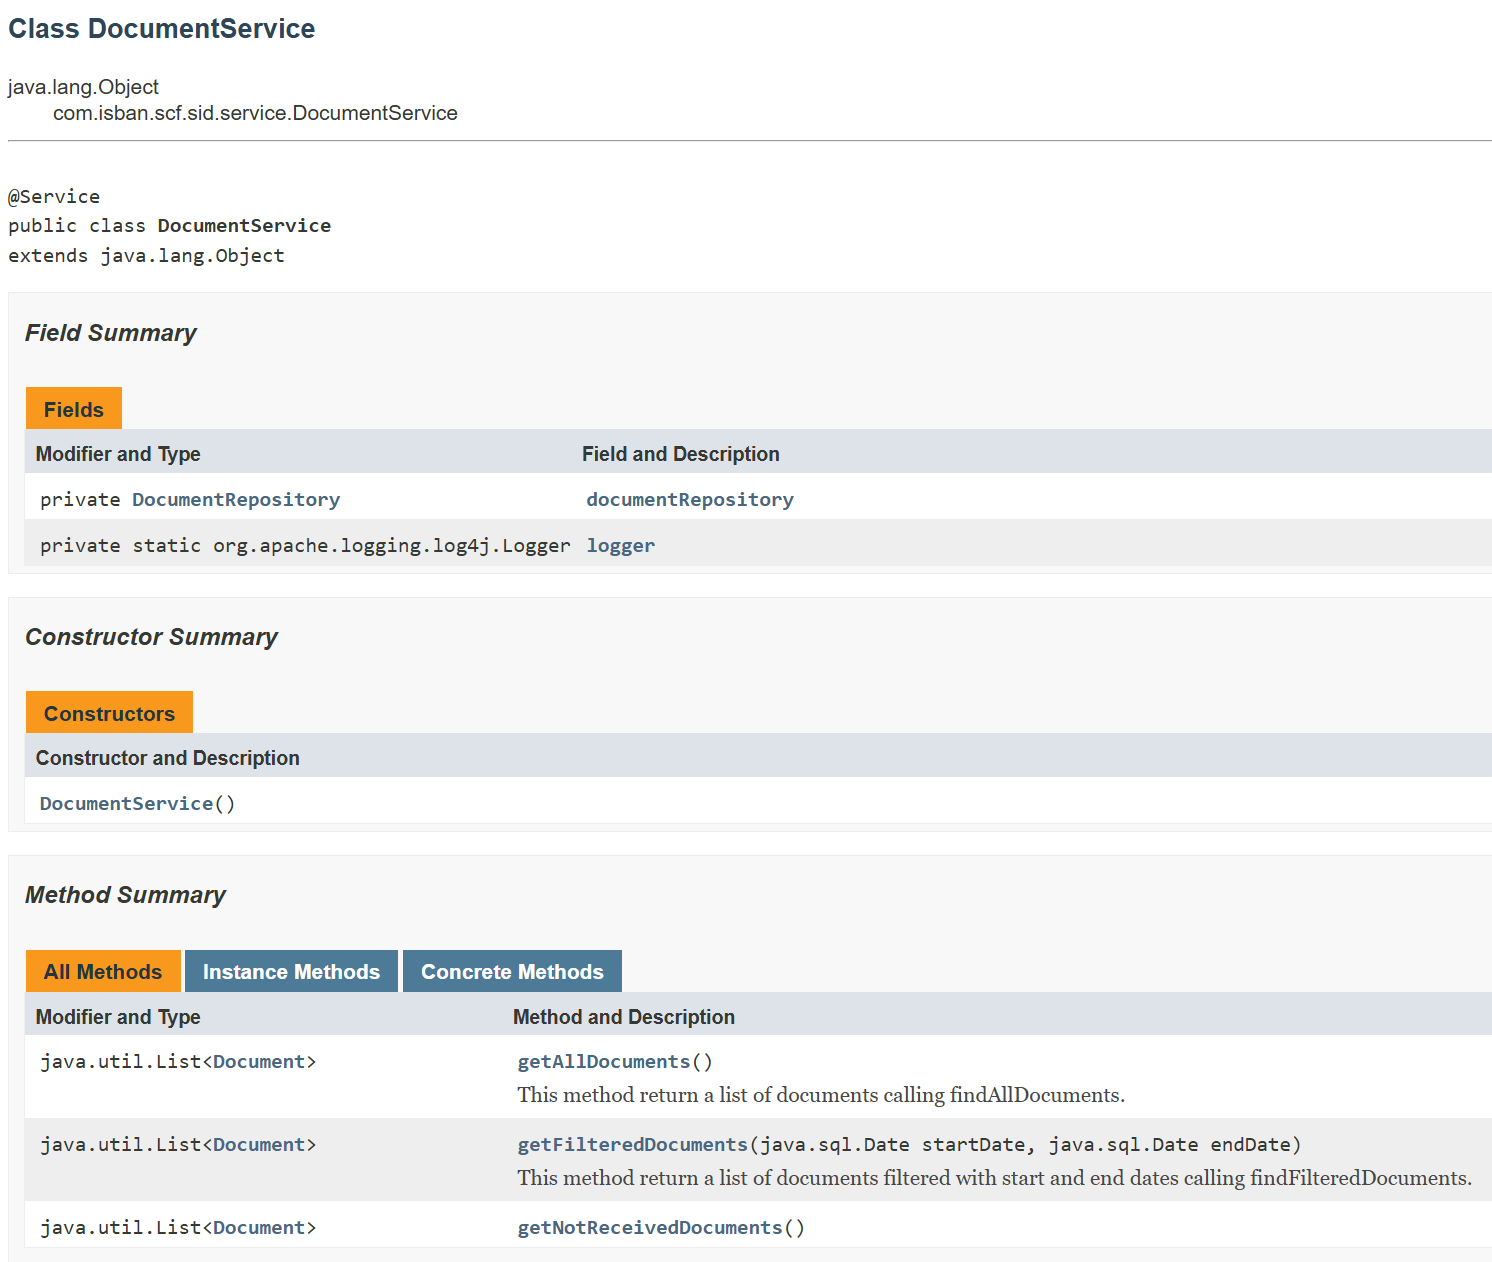
\includegraphics[width=0.5\linewidth]{javadoc-SIDManager.png}
    \caption{Interfaz web de Javadoc para la clase \texttt{DocumentService}}
    \label{fig:javadoc-document-service}
\end{figure}

\subsubsection{Conclusión de documentación}

La implementación de Javadoc en la aplicación no solo mejora la comprensión del código para los desarrolladores, sino que también facilita su uso y mantenimiento. Esta práctica sigue los estándares de la industria y garantiza que cualquier persona que desee utilizar o modificar la aplicación pueda hacerlo de manera eficiente y con un mínimo de esfuerzo.




\chapter{Pruebas y validación}\label{pruebas}
Las pruebas y la validación son etapas críticas en el desarrollo de cualquier sistema de software, ya que permiten garantizar que la aplicación cumple con los requisitos funcionales y no funcionales, además de asegurar su correcto funcionamiento en diferentes escenarios. En este capítulo, se describen las estrategias y metodologías utilizadas para validar el correcto funcionamiento de SIDManager, así como los resultados obtenidos durante este proceso.

\section{Estrategia de pruebas}
Para garantizar la calidad del software, se ha seguido una estrategia de pruebas que combina técnicas de prueba manual y automatizada. Esta estrategia se ha dividido en tres niveles principales:

\begin{itemize}    
    \item \textbf{Pruebas de integración}: Se han llevado a cabo pruebas para validar la interacción entre los diferentes componentes del sistema, como la conexión entre el backend y la base de datos, o la integración entre los servicios y los controladores. Estas pruebas han sido esenciales para detectar posibles errores en la comunicación entre módulos.
    
    \item \textbf{Pruebas de sistema}: Se han realizado pruebas end-to-end para validar el flujo completo de la aplicación, desde la interacción del usuario con la interfaz hasta la persistencia de datos en la base de datos. Estas pruebas han incluido escenarios como el registro de usuarios, la autenticación, la gestión de documentos y la recuperación de contraseñas.
\end{itemize}

\section{Validación de requisitos}
Durante las pruebas, se ha validado que la aplicación cumple con todos los requisitos, incluyendo:

\begin{itemize}
    \item \textbf{Funcionalidades principales}: Registro y autenticación de usuarios, gestión de documentos, filtrado por fechas y verificación del estado de los documentos.
    \item \textbf{Seguridad}: Validación del cifrado de contraseñas y manejo seguro de sesiones.
    \item \textbf{Rendimiento}: Evaluación del tiempo de respuesta de la aplicación bajo diferentes cargas de trabajo, garantizando un rendimiento óptimo incluso con grandes volúmenes de datos.
\end{itemize}

\section{Resultados de las pruebas}
Las pruebas realizadas han demostrado que SIDManager cumple con los requisitos establecidos y funciona de manera correcta en los escenarios evaluados. No obstante, durante el proceso se identificaron algunos errores, como problemas de rendimiento en la carga de grandes volúmenes de datos y fallos en la validación de fechas en casos extremos. Estos errores fueron corregidos y validados en iteraciones posteriores, asegurando la estabilidad y fiabilidad del sistema.

\chapter{Resultados}\label{resultados}
Los resultados obtenidos en el desarrollo de SIDManager demuestran que la aplicación cumple con los objetivos planteados inicialmente, ofreciendo una solución robusta, segura y escalable para la gestión y monitorización de documentos en entornos empresariales. En este capítulo, se presentan los resultados más relevantes del proyecto, tanto a nivel técnico como funcional.

\section{Resultados técnicos}
\begin{itemize}
    \item \textbf{Arquitectura modular}: La aplicación se ha desarrollado siguiendo una arquitectura basada en capas (vista, controlador, servicio, repositorio), lo que ha facilitado su mantenimiento y escalabilidad.
    \item \textbf{Seguridad implementada}: Se ha logrado un alto nivel de seguridad gracias al uso de Spring Security, el cifrado de contraseñas con BCrypt y la protección contra ataques comunes.
    \item \textbf{Integración de tecnologías modernas}: El uso de Spring Boot, Thymeleaf y JPA ha permitido desarrollar una aplicación eficiente y fácil de mantener.
    \item \textbf{Documentación completa}: El código ha sido documentado utilizando Javadoc, lo que facilita su comprensión y mantenimiento por parte de otros desarrolladores.
\end{itemize}

\section{Resultados funcionales}
\begin{itemize}
    \item \textbf{Gestión de documentos}: La aplicación permite filtrar y visualizar documentos de manera eficiente, verificando su correcto almacenamiento en la base de datos.
    \item \textbf{Autenticación y registro}: Los usuarios pueden registrarse, confirmar sus cuentas mediante correo electrónico y autenticarse de manera segura.
    \item \textbf{Recuperación de contraseñas}: Se ha implementado un sistema seguro para la recuperación de contraseñas, utilizando códigos de confirmación únicos.
    \item \textbf{Interfaz intuitiva}: La interfaz de usuario, desarrollada con Thymeleaf y Bootstrap, es clara y fácil de usar, lo que mejora la experiencia del usuario.
\end{itemize}


\chapter{Conclusiones}

Este capítulo sirve como cierre del proyecto y está dividido en dos secciones principales. En la Sección \ref{sec:conclusiones} se presenta un análisis que compara los objetivos alcanzados y aquellos que pueden mejorarse. En la Sección \ref{futuro} se proponen posibles mejoras y líneas de trabajo futuro, tanto en términos de investigación como de desarrollo adicional de la aplicación, además de una reflexión personal sobre el proceso de desarrollo.

\section{Conclusiones}
\label{sec:conclusiones}

El desarrollo de este proyecto ha sido una experiencia enriquecedora que ha permitido aplicar y consolidar conocimientos técnicos, así como aprender nuevas tecnologías y metodologías. A continuación, se resumen las principales conclusiones obtenidas:

\begin{itemize}
    \item \textbf{Planificación y organización}: Hacer las cosas bien desde el principio ahorra tiempo y esfuerzo a largo plazo. Por ejemplo, la implementación de logs propios y el uso de archivos externos para mensajes de la aplicación han demostrado ser decisiones acertadas que facilitaron el mantenimiento y la depuración del código.
    
    \item \textbf{Subestimación de tecnologías}: Durante el desarrollo, se observó que algunas tecnologías o tareas aparentemente simples pueden resultar más complejas de lo esperado. Esto subraya la importancia de investigar y planificar adecuadamente antes de implementar soluciones.
    
    \item \textbf{Documentación y buenas prácticas}: Nombrar variables y clases de manera significativa y seguir estándares de codificación ha sido fundamental para mantener un código legible y fácil de mantener, especialmente en un proyecto con más de 60 archivos editados.
    
    \item \textbf{Importancia de la modularidad}: Separar los mensajes de la aplicación en archivos externos desde el principio ha demostrado ser una práctica muy útil, ya que evita la necesidad de modificar el código fuente cada vez que se requiere un cambio en los textos.

        \item \textbf{Uso de tecnologías modernas}: La elección de tecnologías como  Thymeleaf, en lugar de REST para el backend ha permitido aprovechar al máximo el potencial de SpringBoot. Sin embargo no ha permitido desacoplar el frontend del backend en su totalidad, lo que podría probocar problemas en  la escalabilidad y la integración con frameworks modernos como React o Angular.
\end{itemize}

En resumen, este proyecto ha sido una oportunidad para aplicar conocimientos previos, aprender nuevas herramientas y adoptar buenas prácticas de desarrollo. Aunque se han alcanzado los objetivos principales, siempre hay margen para mejorar y optimizar el trabajo realizado.

\section{Líneas de trabajo futuras}
\label{futuro}

A lo largo del desarrollo del proyecto, surgieron varias ideas y mejoras que, debido a limitaciones de tiempo y alcance, no pudieron implementarse. A continuación, se proponen algunas líneas de trabajo futuro para continuar mejorando la aplicación:

\begin{itemize}
    \item \textbf{Implementación de un framework moderno para el frontend}: Utilizar tecnologías como Vite, Next.js o un framework similar para el desarrollo del frontend, aprovechando el controlador REST ya implementado. Esto mejoraría la experiencia del usuario y facilitaría la creación de interfaces más dinámicas y responsivas.
    
    \item \textbf{Paginación en la carga de documentos}: Implementar un sistema de paginación para la carga de documentos, lo que mejoraría el rendimiento de la aplicación al manejar grandes volúmenes de datos.
    
    \item \textbf{Buscador avanzado}: Implementar un sistema de búsqueda avanzada que permita a los usuarios introducir identificadores específicos (como client\_app\_id o client\_doc\_id) para filtrar y localizar documentos de manera rápida y precisa. Esta funcionalidad mejoraría la usabilidad de la aplicación al permitir búsquedas más eficientes y reducir el tiempo necesario para encontrar información específica.
    
    \item \textbf{Sistema de descarga de datos}: Implementar un sistema integrado en la aplicación para facilitar la descarga de conjuntos de datos de la tabla con los documentos filtrados.
\end{itemize}

Estas propuestas representan oportunidades para seguir avanzando en el desarrollo de la aplicación y explorar nuevas áreas de investigación. La implementación de estas mejoras no solo mejoraría la funcionalidad y usabilidad de la aplicación, sino que también abriría nuevas posibilidades para su uso en entornos académicos y profesionales.

\subsection{Reflexión personal}

Personalmente, este proyecto ha sido una oportunidad para profundizar en tecnologías y conceptos que no formaban parte de mi conocimiento previo. Desde el aprendizaje de nuevas herramientas como Spring Boot y Maven hasta la adopción de buenas prácticas como la documentación con Javadoc y el uso de estándares de Java, he adquirido habilidades que serán valiosas en futuros proyectos. Además, la experiencia de trabajar en un proyecto de esta envergadura ha reforzado mi capacidad para planificar, organizar y resolver problemas de manera eficiente.

En conclusión, este proyecto no solo ha cumplido con sus objetivos iniciales, sino que también ha sentado las bases para futuras mejoras y desarrollos. Espero que el trabajo realizado contribuya al avance de aplicaciones similares y sirva como referencia para otros desarrolladores e investigadores.




%%\nocite{*} %incluye TODOS los documentos de la base de datos bibliográfica sean o no citados en el texto
\newpage
\printbibliography

%\bibliography{bibliografia/bibliografia}
%\addcontentsline{toc}{chapter}{Bibliografía} %sustituir bibliografía con el nombre del fichero bibtex con la bibliografía
%


\appendix
\chapter{Anexo I. Esquema de base de datos}
Aquí vendría el anexo I 

\chapter{Anexo II. Otros...}
Aquí vendría el anexo II 


\addcontentsline{toc}{chapter}{Glosario} %si se usa glosario hay que añadirlo al índice
\printnoidxglossary[type=\acronymtype,title=Glosario]


\end{document}
